\documentclass[10pt,a4paper]{article}
\usepackage[utf8]{inputenc}
\usepackage{graphicx}
\def\Pr{\mathop{\rm Pr}}
\usepackage[landscape,margin=1cm]{geometry}
\usepackage[english]{babel}
\usepackage{tikz}
%\setmainfont{Rubik}[Scale=1.0]
\usepackage{algorithm}
\usepackage{algpseudocode}

\usetikzlibrary{arrows,snakes,backgrounds,shapes.geometric}
\title{Neuromatch Academy Pre-Requisite Refresher - Summary Sheet}
\author{Neuromatch}
%\date{July 2019}
\usepackage[default]{raleway}
\usepackage{fontawesome}
\usepackage[T1]{fontenc}

\usepackage{hyperref}
\usepackage{enumitem}
\usepackage{lipsum}

\usepackage{xcolor}
\definecolor{customcolor}{HTML}{616AC5}
\definecolor{alert}{HTML}{CD5C5C}
\definecolor{w3schools}{HTML}{4CAF50}
\definecolor{subbox}{gray}{0.60}
\definecolor{codecolor}{HTML}{FFC300}
\colorlet{xx}{customcolor}


%--------------------------Editor mode.

\usepackage
[citestyle=authoryear,
sorting=nty,	  		%Sorts bibliography by year, name, title
autocite=footnote, 		%Autocite command generates footnotes
autolang=hyphen, 		
mincrossrefs=1, 	
backend=biber]
{biblatex}

\DeclareFieldFormat{postnote}{#1}
\DeclareFieldFormat{multipostnote}{#1}
\DeclareAutoCiteCommand{footnote}[f]{\footcite}{\footcites}

\bibliography{literature}
%----------------------------------------
%--------------------------------------------------------------------------------
\usepackage{tcolorbox}

\tcbuselibrary{most,listingsutf8,minted}

\tcbset{tcbox width=auto,left=1mm,top=1mm,bottom=1mm,
right=1mm,boxsep=1mm,middle=1pt}

\newenvironment{mycolorbox}[2]{%
\begin{tcolorbox}[grow to left by=-1em,grow to right by=-1em,capture=minipage,fonttitle=\large\bfseries, enhanced jigsaw,boxsep=1mm,colback=#1!30!white,on line,tcbox width=auto, toptitle=0mm,colframe=#2,opacityback=0.7,nobeforeafter,title=#2]%
}{\end{tcolorbox}\\[0.2em]}

\newenvironment{subbox}[2]{%
\begin{tcolorbox}[capture=minipage,fonttitle=\scriptsize\bfseries, enhanced jigsaw,boxsep=1mm,colback=#1!30!white,on line,tcbox width=auto,left=0.3em,top=1mm, toptitle=0mm,colframe=#1,opacityback=0.7,nobeforeafter,title=#2]\footnotesize %
}{\normalsize\end{tcolorbox}\vspace{0.1em}}

\newenvironment{multibox}[1]{%
\begin{tcbraster}[raster columns=#1,raster equal height,nobeforeafter,raster column skip=1em,raster left skip=1em,raster right skip=1em]}{\end{tcbraster}}

\newenvironment{textbox}[1]{\begin{mycolorbox}{customcolor}{#1}}{\end{mycolorbox}}

%-------------------------------
\newtcblisting{codebox}[2]{colback=codecolor!5,colframe=codecolor!80!black,listing only, 
minted options={numbers=left,style=tcblatex,fontsize=\normalsize,breaklines,autogobble,linenos,numbersep=1mm},
left=5mm,enhanced,
title=#2, fonttitle=\bfseries,
listing engine=minted,minted language=#1}

%--------------------------------------------------------------------------------
\newcommand{\punkti}{~\lbrack\dots\rbrack~}

\renewenvironment{quote}
               {\list{\faQuoteLeft\phantom{ }}{\rightmargin\leftmargin}%
                \item\relax\scriptsize\ignorespaces}
               {\unskip\unskip\phantom{xx}\faQuoteRight\endlist}
               

%--------------------------------------------------------------------------------
\newcommand{\bgupper}[3]{\colorbox{#1}{\color{#2}\huge\bfseries\MakeUppercase{#3}}}
\newcommand{\bg}[3]{\colorbox{#1}{\bfseries\color{#2}#3}}

\newcommand{\mycommand}[2]{{\ttfamily\detokenize{#1}}~\dotfill{}~{\footnotesize #2}\\}
\newcommand{\sep}{{\scriptsize~\faCircle{ }~}}


\newcommand{\bggreen}[1]{\medskip\bgupper{w3schools}{black}{#1}\\[0.5em]}
\newcommand{\green}[1]{\smallskip\bg{w3schools}{white}{#1}\\}
\newcommand{\red}[1]{\smallskip\bg{alert}{white}{#1}\\}

\usepackage{multicol}
\setlength{\columnsep}{30pt}

\setlength{\parindent}{0pt}
\pagestyle{empty}

\usepackage{csquotes}

\newcommand{\loremipsum}{Lorem ipsum dolor sit amet.}

\clearpage
%\defaultfontfeatures{ Scale=MatchUppercase, Ligatures=TeX }
%\setmathfont{Fira Math}
%\setmathfont{Rubik}[range=up]
%--------------------------------------------------------------------------------
\begin{document}

%%% BayesianDecisions
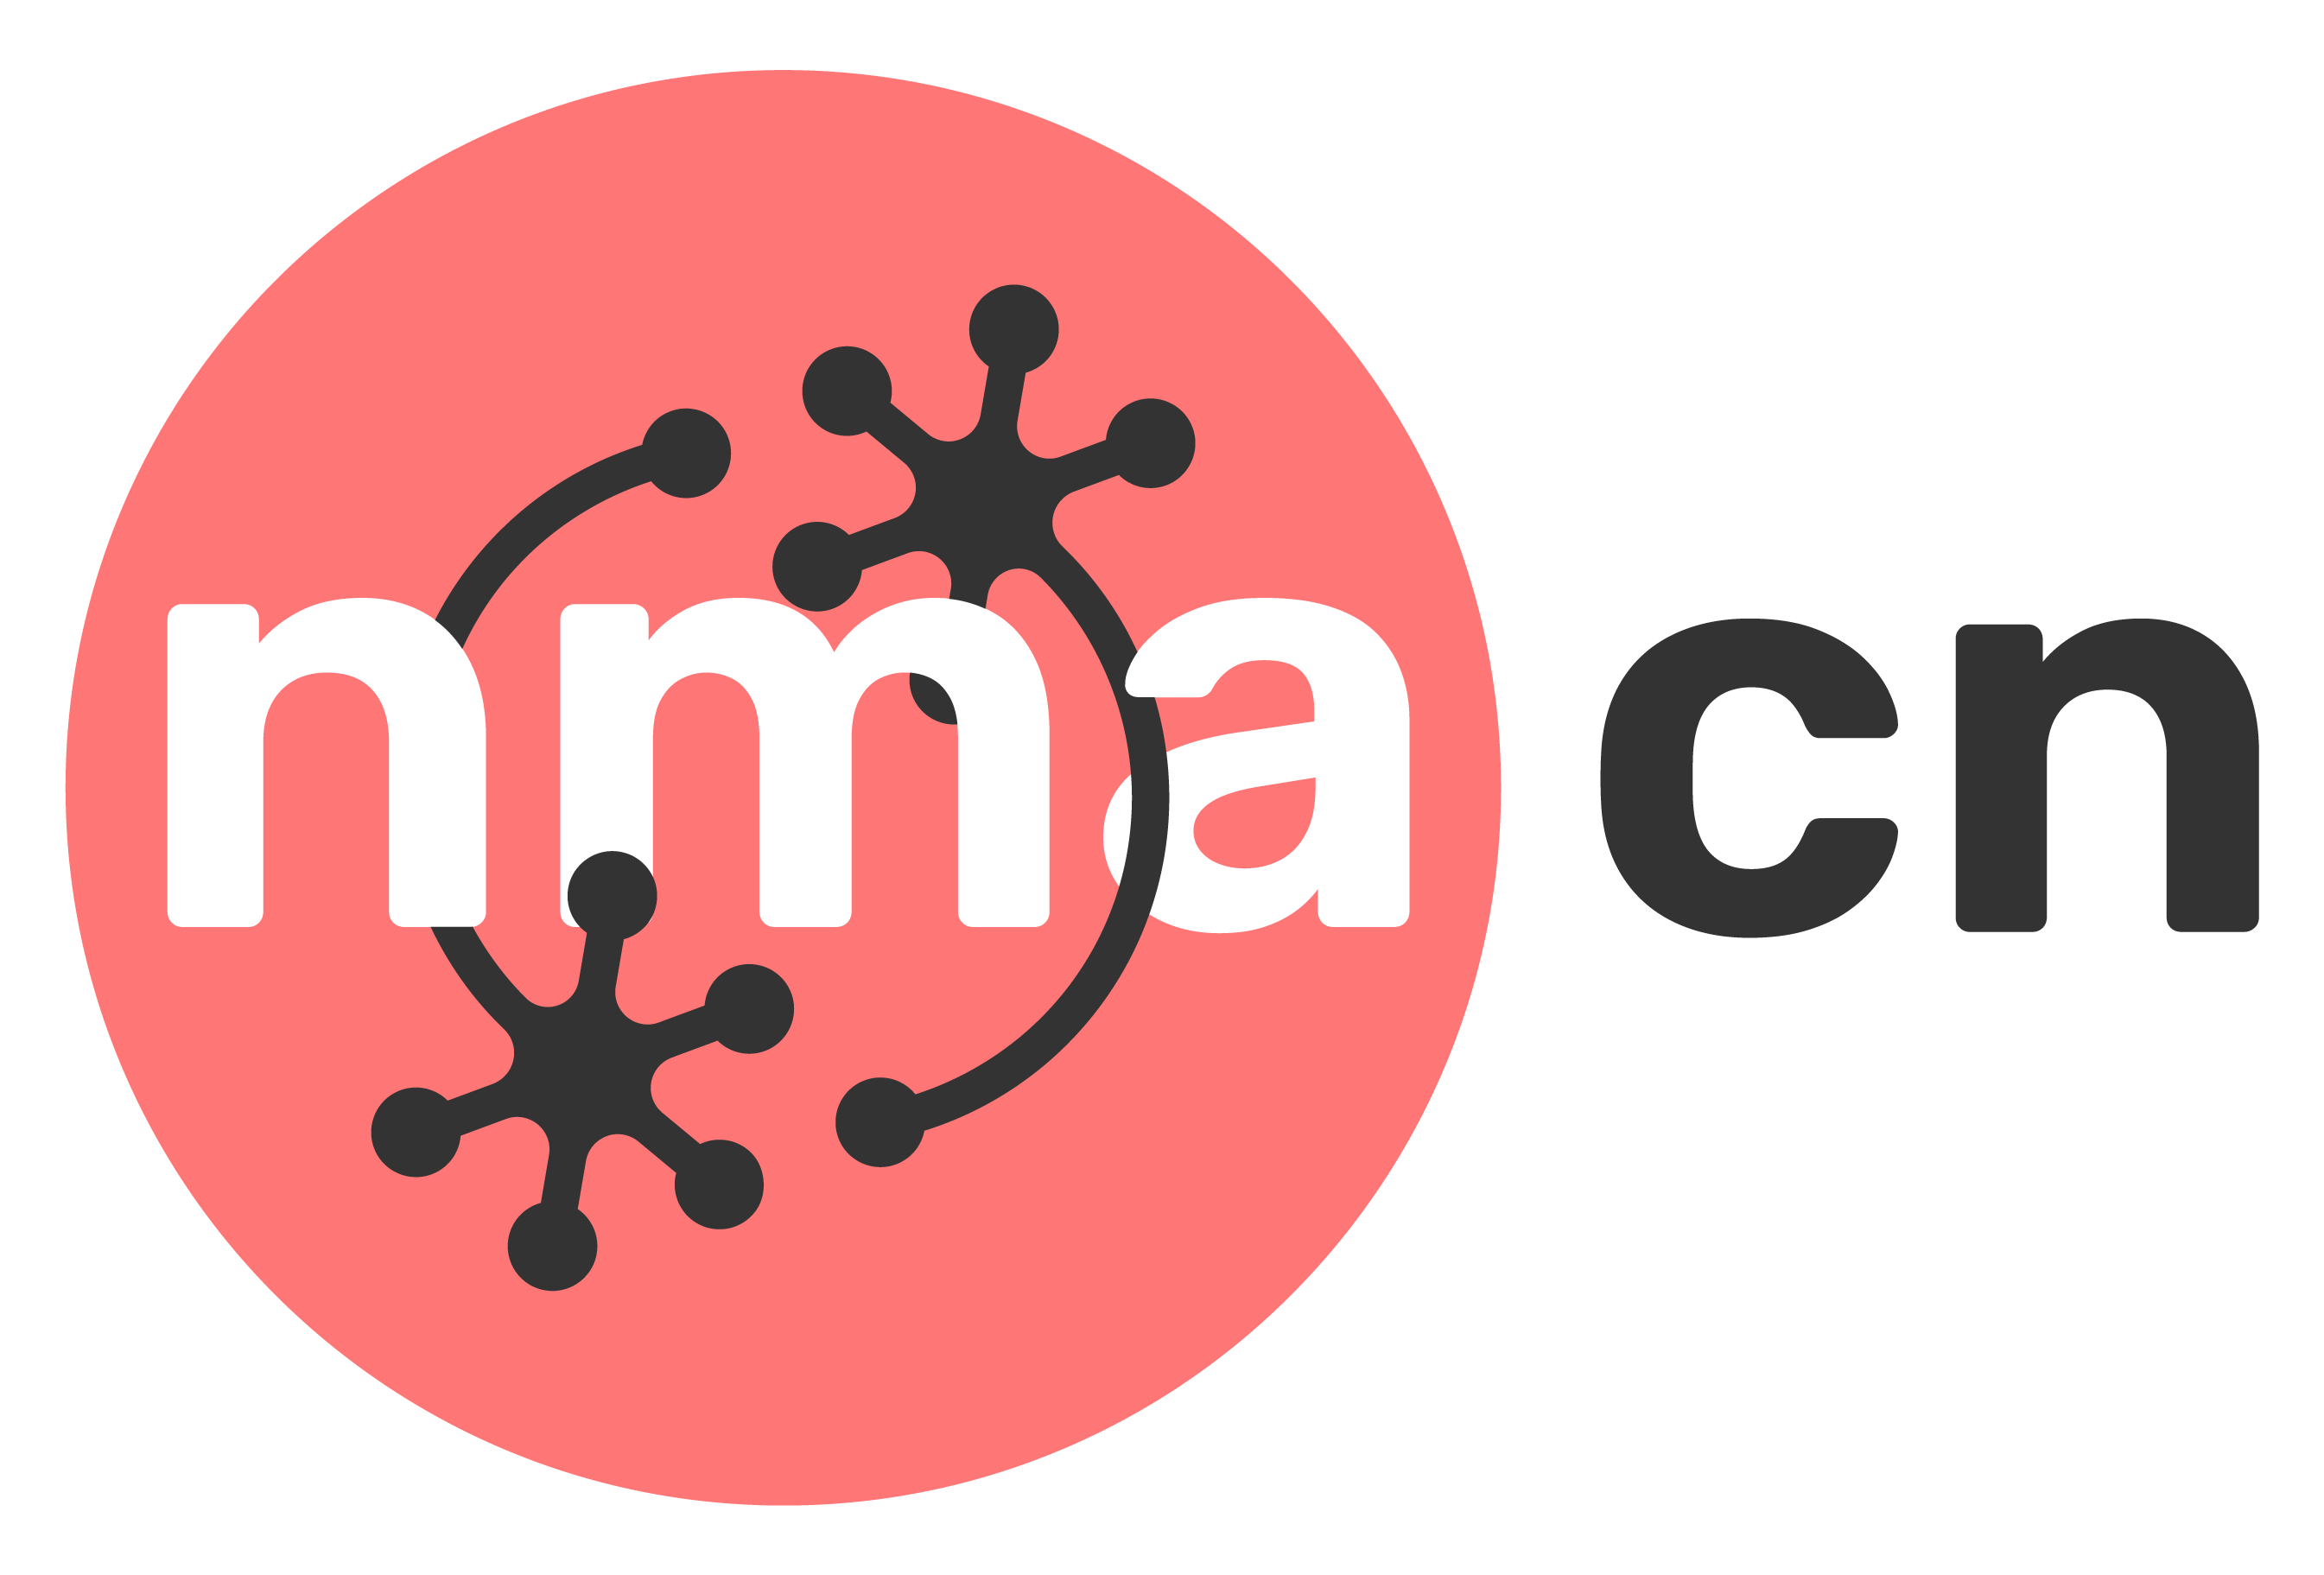
\includegraphics[scale=0.03]{Figures/NMACN.png}\href{https://compneuro.neuromatch.io/tutorials/intro.html}{\textbf{\Huge{Neuromatch Academy: Bayesian Decisions - Summary Sheet}}\footnote{’t Hart et al., (2022). Neuromatch Academy: a 3-week, online summer school in computational neuroscience. Journal of Open Source Education, 5(49), 118. https://doi.org/10.21105/jose.00118}}
%$\subsection*{Cheat Sheet}
\small
\begin{multicols}{3}

\let\clearpage\relax
\clearpage
\begin{textbox}{\href{https://compneuro.neuromatch.io/tutorials/W3D1_BayesianDecisions/student/W3D1_Tutorial1.html}{Bayes with a binary hidden state (W3D1T1)} }
\begin{subbox}{subbox}{Introduction}
\scriptsize

We will introduce the fundamental building blocks for Bayesian statistics: 

1. How do we combine the possible loss (or gain) for making a decision with our probabilistic knowledge?\\
2. 
 How do we use probability distributions to represent hidden states?\\
3. How does marginalization work and how can we use it?\\
 4. How do we combine new information with our prior knowledge? 

\end{subbox}

\begin{subbox}{subbox}{Gone Fishin'}
\scriptsize
We are going to explore \textbf{binary hidden state problem} by going fishing. We need to decide which side to fish on--the hidden state. We know fish like to school together. On different days the school of fish is either on the left or right side, but we don’t know what the case is today. We define our knowledge about the fish location as a distribution over the random hidden state variable. Using our probabilistic knowledge, also called our \textbf{belief} about the hidden state, we will explore how to make the decision about where to fish today, based on what to expect in terms of gains or losses for the decision.
The gains and loss are defined by the utility of choosing an action, which is fishing on the left or right. 

\end{subbox}
\begin{subbox}{subbox}{Deciding where to fish}
\scriptsize

Let's start to get a sense of how all this works using an example. First, make sure we understand how the expected utility of each action is being computed from the probabilities and the utility values. In the initial state: the probability of the fish being on the left is 0.9 and on the right is 0.1. The expected utility of the action of fishing on the left is then $U(s = \textrm{left},a = \textrm{left})p(s = \textrm{left}) + U(s = \textrm{right},a = \textrm{left})p(s = \textrm{right}) = 2(0.9) + -2(0.1) = 1.6$. Essentially, to get the expected utility of action $a$, we are doing a weighted sum over the relevant column of the utility matrix (corresponding to action $a$) where the weights are the state probabilities.

\centering
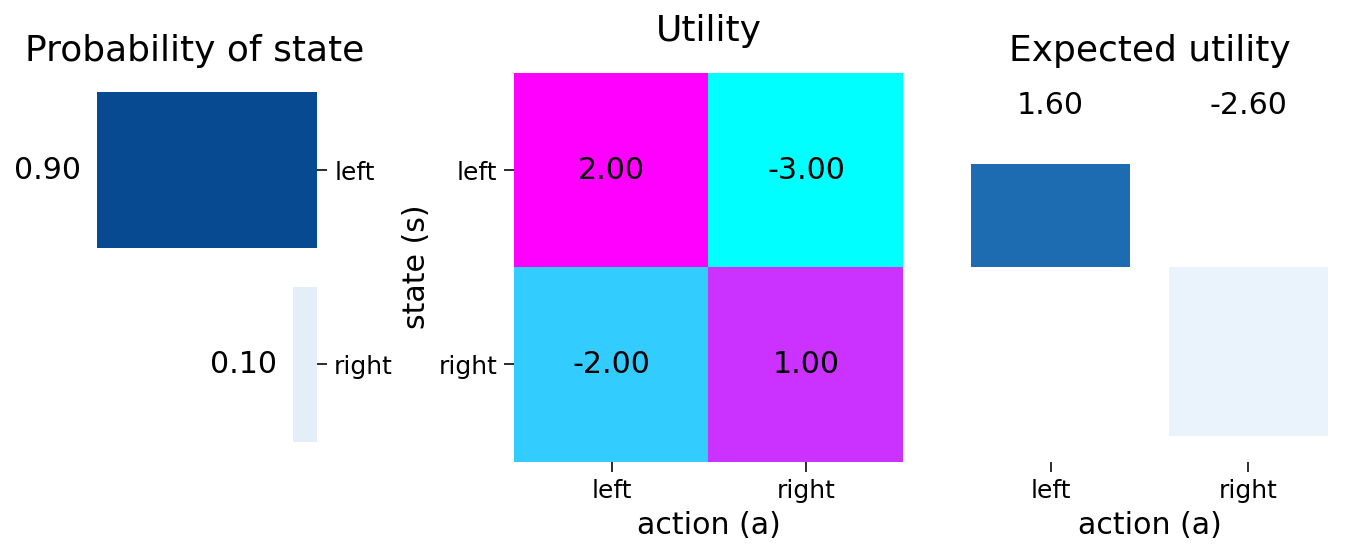
\includegraphics[scale=0.23]{Figures/BD/BD_Figure1.png}

\end{subbox}
\end{textbox}
%%%%%%%%%%%%%%%%%%%%%%%%%%%%%%%%%%%%%%%%%%%%%%%%%%
%%%%%%%%%%%%%%%%%%%%%%%%%%%%%%%%%%%%%%%%%%%%%%%%%%
\begin{textbox}{\href{https://compneuro.neuromatch.io/tutorials/W3D1_BayesianDecisions/student/W3D1_Tutorial1.html}{Bayes with a binary hidden state (W3D1T1)} }
\begin{subbox}{subbox}{Likelihood of the fish being on either side}
\scriptsize

First, we'll think about what it means to take a measurement (also often called an observation or just data) and what it tells us about what the hidden state may be. Specifically, we'll be looking at the \textbf{likelihood}, which is the probability of our measurement ($m$) given the hidden state ($s$): $P(m | s)$. Remember that in this case, the hidden state is which side of the dock the school of fish is on.
We will watch someone fish (for let's say 10 minutes) and our measurement is whether they catch a fish or not. We know something about what catching a fish means for the likelihood of the fish being on one side or the other.

\end{subbox}

\begin{subbox}{subbox}{Guessing the location of the fish}
\scriptsize
Let's say we go to a different dock to fish. Here, there are different probabilities of catching fish given the state of the world. At this dock, if we fish on the side of the dock where the fish are, we have a 70\% chance of catching a fish. If we fish on the wrong side, we will catch a fish with only 20\% probability. These are the likelihoods of observing someone catching a fish! That is, we are taking a measurement by seeing if someone else catches a fish!

\textit{We see a fisher-person is fishing on the left side.}
 
In the example, we tried to guess where the school of fish was based on the measurement we took (watching someone fish). We did this by choosing the state (side where we think the fish are) that maximized the probability of the measurement. In other words, we estimated the state by maximizing the likelihood (the side with the highest probability of measurement given state $P(m|s$)). This is called maximum likelihood estimation (MLE).

But, what if we had been going to this dock for years and we knew that the fish were almost always on the left side? This should probably affect how we make our estimate -- we would rely less on the single new measurement and more on our prior knowledge. This is the fundamental idea behind Bayesian inference.

\end{subbox}

\end{textbox}
%%%%%%%%%%%%%%%%%%%%%%%%%%%%%%%%%%%%%%%%%%%%%%%%%%
%%%%%%%%%%%%%%%%%%%%%%%%%%%%%%%%%%%%%%%%%%%%%%%%%%
\begin{textbox}{\href{https://compneuro.neuromatch.io/tutorials/W3D1_BayesianDecisions/student/W3D1_Tutorial1.html}{Bayes with a binary hidden state (W3D1T1)} }
\begin{subbox}{subbox}{Correlation}
\scriptsize

We are going to take a step back for a bit and think more generally about the amount of information shared between two random variables. We want to know how much information we gain when we observe one variable (take a measurement) if we know something about another. We will see that the fundamental concept is the same if we think about two attributes, for example the size and color of the fish, or the prior information and the likelihood.

\end{subbox}
\begin{subbox}{subbox}{Covarying probability distributions
}
\scriptsize

The relationship between the marginal probabilities and the joint probabilities is determined by the correlation between the two random variables - a normalized measure of how much the variables covary. We can also think of this as gaining some information about one of the variables when we observe a measurement from the other.  

Here, we want to think about how the correlation between size and color of these fish changes how much information we gain about one attribute based on the other. 

\centering
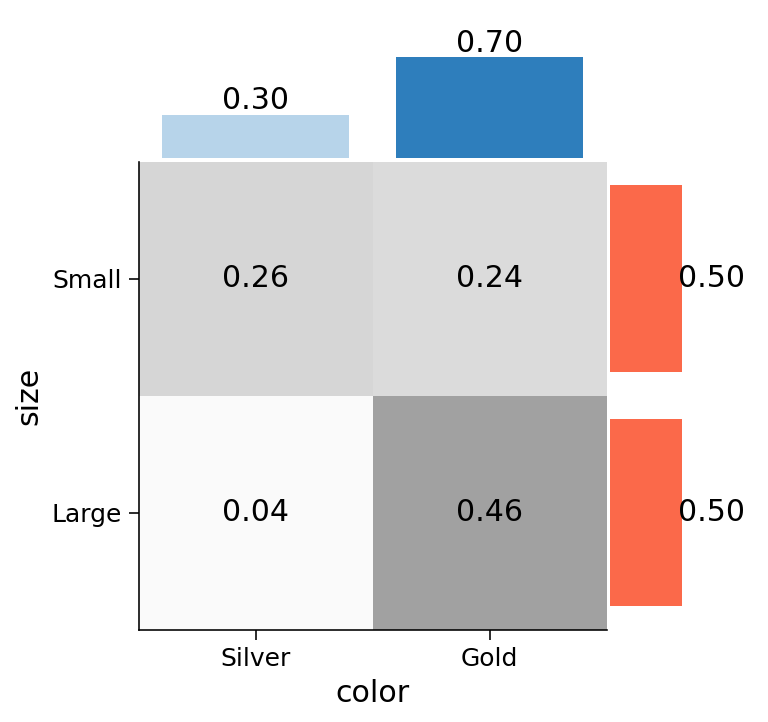
\includegraphics[scale=0.35]{Figures/BD/BD_Figure2.png}

\end{subbox}


\end{textbox}
%%%%%%%%%%%%%%%%%%%%%%%%%%%%%%%%%%%%%%%%%%%%%%%%%%
%%%%%%%%%%%%%%%%%%%%%%%%%%%%%%%%%%%%%%%%%%%%%%%%%%

\begin{textbox}{\href{https://compneuro.neuromatch.io/tutorials/W3D1_BayesianDecisions/student/W3D1_Tutorial1.html}{Bayes with a binary hidden state (W3D1T1)} }
\begin{subbox}{subbox}{Marginalisation}
\scriptsize
We may want to find the probability of one variable while ignoring another: we will do this by averaging out, or marginalizing, the irrelevant variable.

We will think of this in two different ways.

In the first math exercise, we will think about the case where we know the joint probabilities of two variables and want to figure out the probability of just one variable. To make this explicit, let's assume that a fish has a color that is either gold or silver (our first variable) and a size that is either small or large (our second). We could write out the the \textbf{joint probabilities}: the probability of both specific attributes occuring together. For example, the probability of a fish being small and silver, $P(X = \textrm{small}, Y = \textrm{silver})$, is 0.4. The following table summarizes our joint probabilities:

\begin{center}
\begin{tabular}{||c c c||} 
 \hline
 P(X, Y) & Y = silver & Y = gold \\ [0.5ex] 
 \hline\hline
 X = small & 0.4 & 0.2\\ 
 \hline
 X = large & 0.1  & 0.3  \\ [1ex] 
 \hline
\end{tabular}
\end{center}
We want to know what the probability of a fish being small  regardless of color. Since the fish are either silver or gold, this would be the probability of a fish being small and silver plus the probability of a fish being small and gold. This is an example of marginalizing, or averaging out, the variable we are not interested in across the rows or columns.. In math speak: $P(X = \textrm{small}) = \sum_y{P(X = \textrm{small}, Y)}$. This gives us a \textbf{marginal probability}, a probability of a variable outcome (in this case size), regardless of the other variables (in this case color).

More generally, we can marginalize out a second irrelevant variable $y$ by summing over the relevant joint probabilities:

$$p(x) = \sum_y p(x, y) $$

To find the marginal probability of a measurement we will remove an unknown (the hidden state). We will do this by marginalizing out the hidden state. In this case, we know the conditional probabilities of the measurement given state and the probabilities of each state. We can marginalize using:

$$p(m) = \sum_s p(m | s) p(s) $$

These two ways of thinking about marginalization (as averaging over joint probabilities or conditioning on some variable) are equivalent because the joint probability of two variables equals the conditional probability of the first given the second times the marginal probability of the second:

$$p(x, y) = p(x|y)p(y)$$ 


\end{subbox}

\end{textbox}
%%%%%%%%%%%%%%%%%%%%%%%%%%%%%%%%%%%%%%%%%%%%%%%%%%
%%%%%%%%%%%%%%%%%%%%%%%%%%%%%%%%%%%%%%%%%%%%%%%%%%
\begin{textbox}{\href{https://compneuro.neuromatch.io/tutorials/W3D1_BayesianDecisions/student/W3D1_Tutorial1.html}{Bayes with a binary hidden state (W3D1T1)} }
\begin{subbox}{subbox}{Computing marginal probabilities}
\scriptsize

 The probability of a fish being silver is the joint probability of it being
     small and silver plus the joint probability of it being large and silver:
\begin{eqnarray*}
 P(Y = silver) =\\ 
 P(X = small, Y = silver) + P(X = large, Y = silver)\\
                  = 0.4 + 0.1
                  = 0.5
                  \end{eqnarray*} 
This is all the possibilities as in this scenario, our fish can only be small
   or large, silver or gold. So the probability is 1 - the fish has to be at
   least one of these.\\
 First we compute the marginal probabilities
\begin{align*} P(X = small) =\\ P(X = small, Y = silver) + P(X = small, Y = gold)\\ = 0.4+0.2=0.6\end{align*} 
\begin{align*}  P(Y = gold) = \\P(X = small, Y = gold) + P(X = large, Y = gold) = 0.5\end{align*} 
   We already know the joint probability: \begin{align*} P(X = small, Y = gold) = 0.2\end{align*} 
   We can now use the given formula:
\begin{align*}    P( X = small or Y = gold) = \\P(X = small) + P(Y = gold) - P(X = small, Y = gold)\\
                             = 0.6 + 0.5 - 0.2
                             = 0.9 \end{align*} 
                             
                    

\end{subbox}
\begin{subbox}{subbox}{Computing marginal likelihood}
\scriptsize
When we normalize to find the posterior, we need to determine the marginal likelihood--or evidence--for the measurement we observed. To do this, we need to marginalize as we just did above to find the probabilities of a color or size. Only, in this case, we are marginalizing to remove a conditioning variable! In this case, let's consider the likelihood of fish (if we observed a fisher-person fishing on the \textit{right}).

\begin{center}
\begin{tabular}{||c c c||} 
 \hline
 p(m\|s)  & m = fish & m = no fish \\ [0.5ex] 
 \hline\hline
s = left & 0.1 & 0.9\\ 
 \hline
s = right & 0.5  & 0.5  \\ [1ex] 
 \hline
\end{tabular}
\end{center}
The table above shows us the \textbf{likelihoods}, just as we explored earlier.

We want to know the total probability of a fish being caught, $P(m = \textrm{fish})$, by the fisher-person fishing on the right. (We would need this to calculate the posterior.) To do this, we will need to consider the prior probability, $p(s)$, and marginalize over the hidden states!

This is an example of marginalizing, or conditioning away, the variable we are not interested in as well.


\end{subbox}

\end{textbox}
%%%%%%%%%%%%%%%%%%%%%%%%%%%%%%%%%%%%%%%%%%%%%%%%%%
%%%%%%%%%%%%%%%%%%%%%%%%%%%%%%%%%%%%%%%%%%%%%%%%%%
\begin{textbox}{\href{https://compneuro.neuromatch.io/tutorials/W3D1_BayesianDecisions/student/W3D1_Tutorial1.html}{Bayes with a binary hidden state (W3D1T1)} }
\begin{subbox}{subbox}{Computing marginal likelihood}
\scriptsize

Given the priors
Priors
$$P(s = left) = 0.3$$
$$P(s = right) = 0.7$$
and the likelihoods
$$P(m = fish | s = left) = 0.1$$
$$P(m = fish | s = right) = 0.5$$
$$P(m = no fish | s = left) = 0.9$$
$$P(m = no fish | s = right) = 0.5$$

We can calculate the marginal likelihood (evidence):
 \begin{eqnarray*}   P(m = fish)\\ 
 = P(m = fish, s = left) + P(m = fish, s = right)\\
                = P(m = fish | s = left)P(s = left) +\\ P(m = fish | s = right)P(s = right)\\
                = 0.1 * 0.3 + .5 * .7
            = 0.38
            \end{eqnarray*}
We can calculate the marginal likelihood (evidence): 
  \begin{eqnarray*}    P(m = fish) =\\ P(m = fish, s = left) + P(m = fish, s = right)
                =\\ P(m = fish | s = left)P(s = left) + \\P(m = fish | s = right)P(s = right)\\
                = 0.1 * 0.6 + .5 * .4
                = 0.26
                 \end{eqnarray*} 
\end{subbox}

\end{textbox}
%%%%%%%%%%%%%%%%%%%%%%%%%%%%%%%%%%%%%%%%%%%%%%%%%%
%%%%%%%%%%%%%%%%%%%%%%%%%%%%%%%%%%%%%%%%%%%%%%%%%%
\begin{textbox}{\href{https://compneuro.neuromatch.io/tutorials/W3D1_BayesianDecisions/student/W3D1_Tutorial1.html}{Bayes with a binary hidden state (W3D1T1)} }
\begin{subbox}{subbox}{Bayes' Rule and the Posterior}
\scriptsize
Marginalization is going to be used to combine our prior knowledge, which we call the \textbf{prior}, and our new information from a measurement, the \textbf{likelihood}. Only in this case, the information we gain about the hidden state we are interested in, where the fish are, is based on the relationship between the probabilities of the measurement and our prior. 

We can now calculate the full posterior distribution for the hidden state ($s$) using Bayes' Rule. As we've seen, the posterior is proportional to the prior times the likelihood. This means that the posterior probability of the hidden state ($s$) given a measurement ($m$) is proportional to the likelihood of the measurement given the state times the prior probability of that state:

\begin{equation}
P(s | m) \propto P(m | s) P(s)
\end{equation}

We say proportional to instead of equal because we need to normalize to produce a full probability distribution:

\begin{equation}
P(s | m) = \frac{P(m | s) P(s)}{P(m)}
\end{equation}

Normalizing by this $P(m)$ means that our posterior is a complete probability distribution that sums or integrates to 1 appropriately. We now can use this new, complete probability distribution for any future inference or decisions we like! In fact, as we will see tomorrow, we can use it as a new prior! Finally, we often call this probability distribution our beliefs over the hidden states, to emphasize that it is our subjective knowledge about the hidden state.

For many complicated cases, like those we might be using to model behavioral or brain inferences, the normalization term can be intractable or extremely complex to calculate. We can be careful to choose probability distributions where we can analytically calculate the posterior probability or numerical approximation is reliable. Better yet, we sometimes don't need to bother with this normalization! The normalization term, $P(m)$, is the probability of the measurement. This does not depend on state so is essentially a constant we can often ignore. We can compare the unnormalized posterior distribution values for different states because how they relate to each other is unchanged when divided by the same constant. We will see how to do this to compare evidence for different hypotheses tomorrow. (It's also used to compare the likelihood of models fit using maximum likelihood estimation)

In this relatively simple example, we can compute the marginal likelihood $P(m)$ easily by using:

\begin{equation}
P(m) = \sum_s P(m | s) P(s)
\end{equation}

We can then normalize so that we deal with the full posterior distribution.
 
\end{subbox}

\end{textbox}

%%%%%%%%%%%%%%%%%%%%%%%%%%%%%%%%%%%%%%%%%%%%%%%%%%
%%%%%%%%%%%%%%%%%%%%%%%%%%%%%%%%%%%%%%%%%%%%%%%%%%

\begin{textbox}{\href{https://compneuro.neuromatch.io/tutorials/W3D1_BayesianDecisions/student/W3D1_Tutorial1.html}{Bayes with a binary hidden state (W3D1T1)} }
\begin{subbox}{subbox}{Calculating a posterior probability
}
\scriptsize

Given the priors
Priors
$$P(s = left) = 0.3$$
$$P(s = right) = 0.7$$
and the likelihoods
$$P(m = fish | s = left) = 0.1$$
$$P(m = fish | s = right) = 0.5$$
$$P(m = no fish | s = left) = 0.9$$
$$P(m = no fish | s = right) = 0.5$$

Calculate the posterior probability that the school is on the left if the fisher-person catches a fish: $p(s = \textrm{left} | m = \textrm{fish})$ (hint: normalize by computing $p(m = \textrm{fish})$).

Using Bayes rule, we know that 
\begin{eqnarray*}   
P(s = left | m = fish) \\ 
 = \frac{P(m = fish | s = left)P(s = left)}{P(m = fish)}
            \end{eqnarray*}
Let's first compute P(m = fish):
\begin{eqnarray*}   
   P(m = fish) =  \\
   P(m = fish | s = left)P(s = left) + \\ P(m = fish | s = right)P(s = right)\\
               = 0.5 * 0.3 + .1 * .7
               = 0.22
                \end{eqnarray*}
   Now we can plug in all parts of Bayes rule:
\begin{eqnarray*}     P(s = left | m = fish) =\\
\frac{P(m = fish | s = left)P(s = left) }{ P(m = fish)}
                          = \frac{0.5 * 0.3 }{ 0.22}
                          = 0.68
                          \end{eqnarray*}
Calculate the posterior probability that the school is on the right if the fisher-person does not catch a fish: $p(s = \textrm{right} | m = \textrm{no fish})$. Using Bayes rule, we know that 
\begin{eqnarray*} P(s = right | m = no fish) =\\ \frac{P(m = no fish | s = right)P(s = right) }{ P(m = no fish)}\end{eqnarray*} 
   Let's first compute P(m = no fish):
\begin{eqnarray*}    P(m = no fish) = \\P(m = no fish | s = left)P(s = left) +  \\P(m = no fish | s = right)P(s = right)\\
                  = 0.5 * 0.3 + .9 * .7
                  = 0.78
                  \end{eqnarray*} 
   Now we can plug in all parts of Bayes rule:
 \begin{eqnarray*}    P(s = right | m = no fish) = \\
 \frac{P(m = no fish | s = right)P(s = right) }{ P(m = no fish)}\\
                              = \frac{0.9 * 0.7 }{ 0.78}
                              = 0.81
\end{eqnarray*}  
\end{subbox}

\end{textbox}
%%%%%%%%%%%%%%%%%%%%%%%%%%%%%%%%%%%%%%%%%%%%%%%%%%
%%%%%%%%%%%%%%%%%%%%%%%%%%%%%%%%%%%%%%%%%%%%%%%%%%
\begin{textbox}{\href{https://compneuro.neuromatch.io/tutorials/W3D1_BayesianDecisions/student/W3D1_Tutorial1.html}{Bayes with a binary hidden state (W3D1T1)} }
\begin{subbox}{subbox}{Computing Posteriors}
\scriptsize
Let's implement our above math to be able to compute posteriors for different priors and likelihoods in graphical form.

\centering
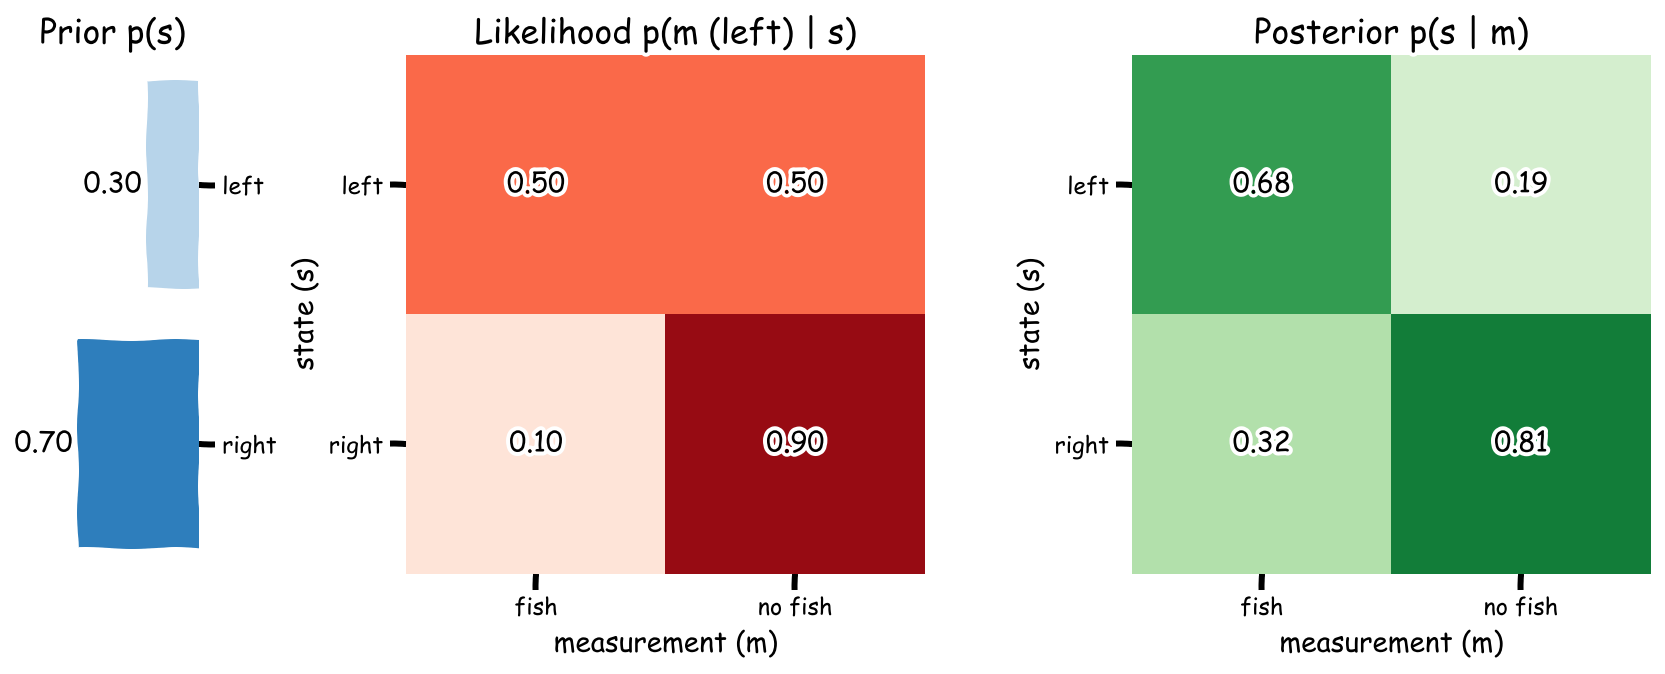
\includegraphics[scale=0.12]{Figures/BD/BD_Figure3.png}

 
\end{subbox}

\begin{subbox}{subbox}{Making Bayesian fishing decisions}
\scriptsize
We consider the expected utility of an action based on our belief (the posterior distribution) about where we think the fish are. Now we have all the components of a Bayesian decision: our prior information, the likelihood given a measurement, the posterior distribution (belief) and our utility (the gains and losses). This allows us to consider the relationship between the true value of the hidden state, $s$, and what we \textit{expect} to get if we take action, $a$, based on our belief!


\centering
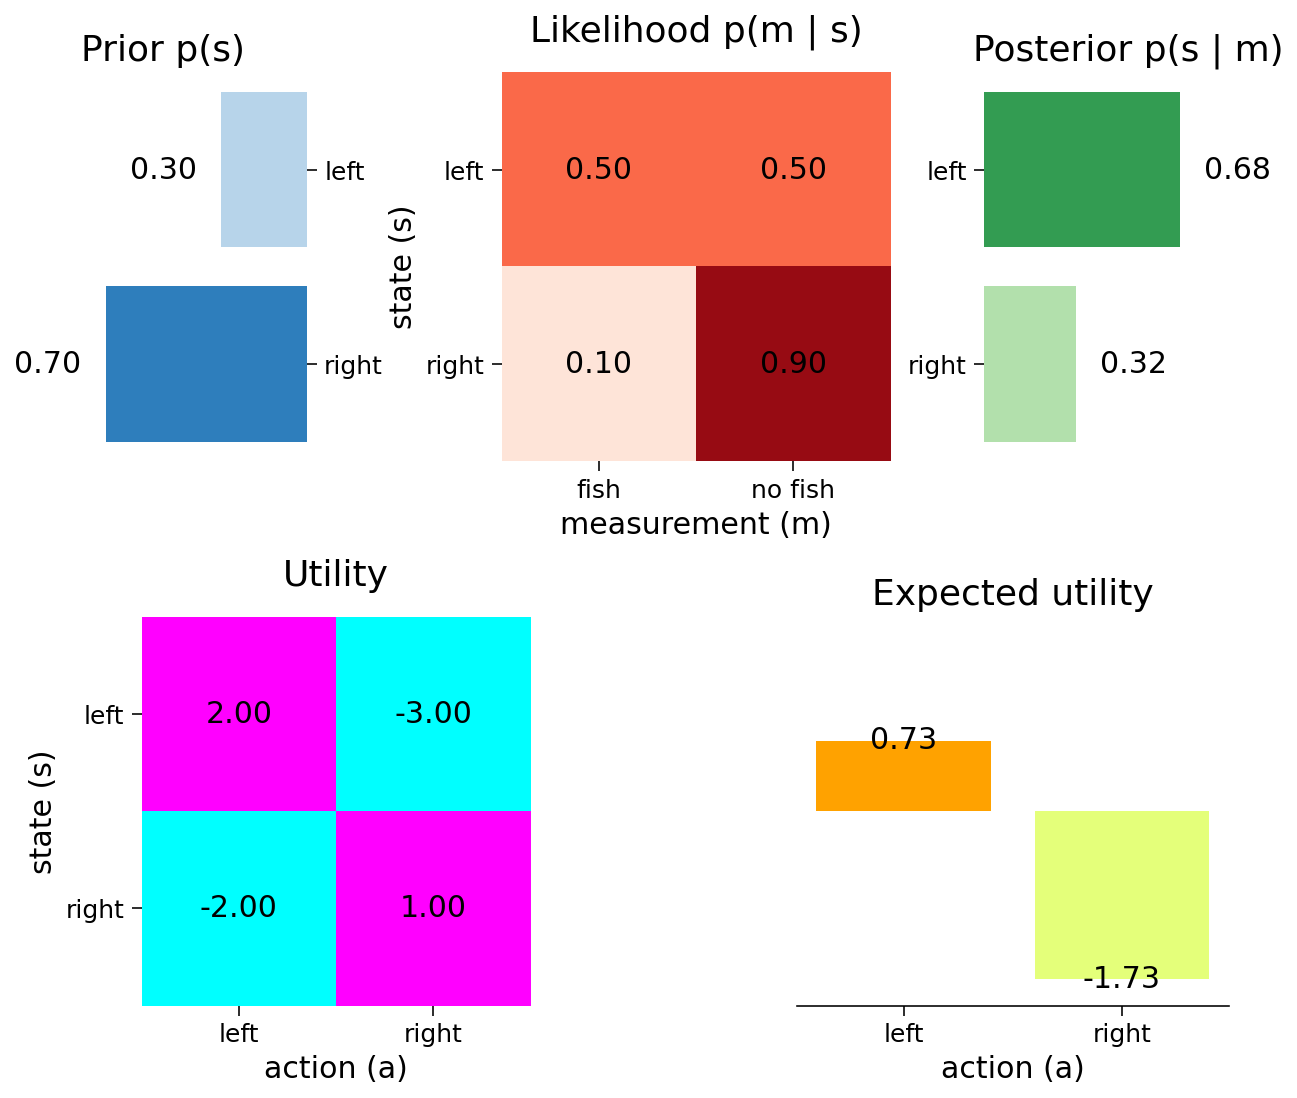
\includegraphics[scale=0.25]{Figures/BD/BD_Figure4.png}

 
\end{subbox}
\end{textbox}
%%%%%%%%%%%%%%%%%%%%%%%%%%%%%%%%%%%%%%%%%%%%%%%%%%
%%%%%%%%%%%%%%%%%%%%%%%%%%%%%%%%%%%%%%%%%%%%%%%%%%
%%% TUTORIAL 2
%%%%%%%%%%%%%%%%%%%%%%%%%%%%%%%%%%%%%%%%%%%%%%%%%%
%%%%%%%%%%%%%%%%%%%%%%%%%%%%%%%%%%%%%%%%%%%%%%%%%%
\begin{textbox}{\href{https://compneuro.neuromatch.io/tutorials/W3D1_BayesianDecisions/student/W3D1_Tutorial2.html}{Bayesian inference and decisions with continuous hidden state (W3D1T2)} }
\begin{subbox}{subbox}{Astrocat!}
\scriptsize
Let's say you are a cat astronaut - Astrocat! You are navigating around space using a jetpack and your goal is to chase a mouse. 

Since you are a cat, you don't have opposable thumbs and cannot control your own jet pack. It can only be controlled by ground control back on Earth. 

For them to be able to guide you, they need to know where you are. They are trying to figure out your location. They have prior knowledge of your location - they know you like to hang out near the space mouse. They can also get an unreliable quick glimpse: they are taking a measurement of the hidden state of your location.

They will try to figure out your location using Bayes rule and Bayesian decisions - as we will see throughout this tutorial.


\begin{center}
    
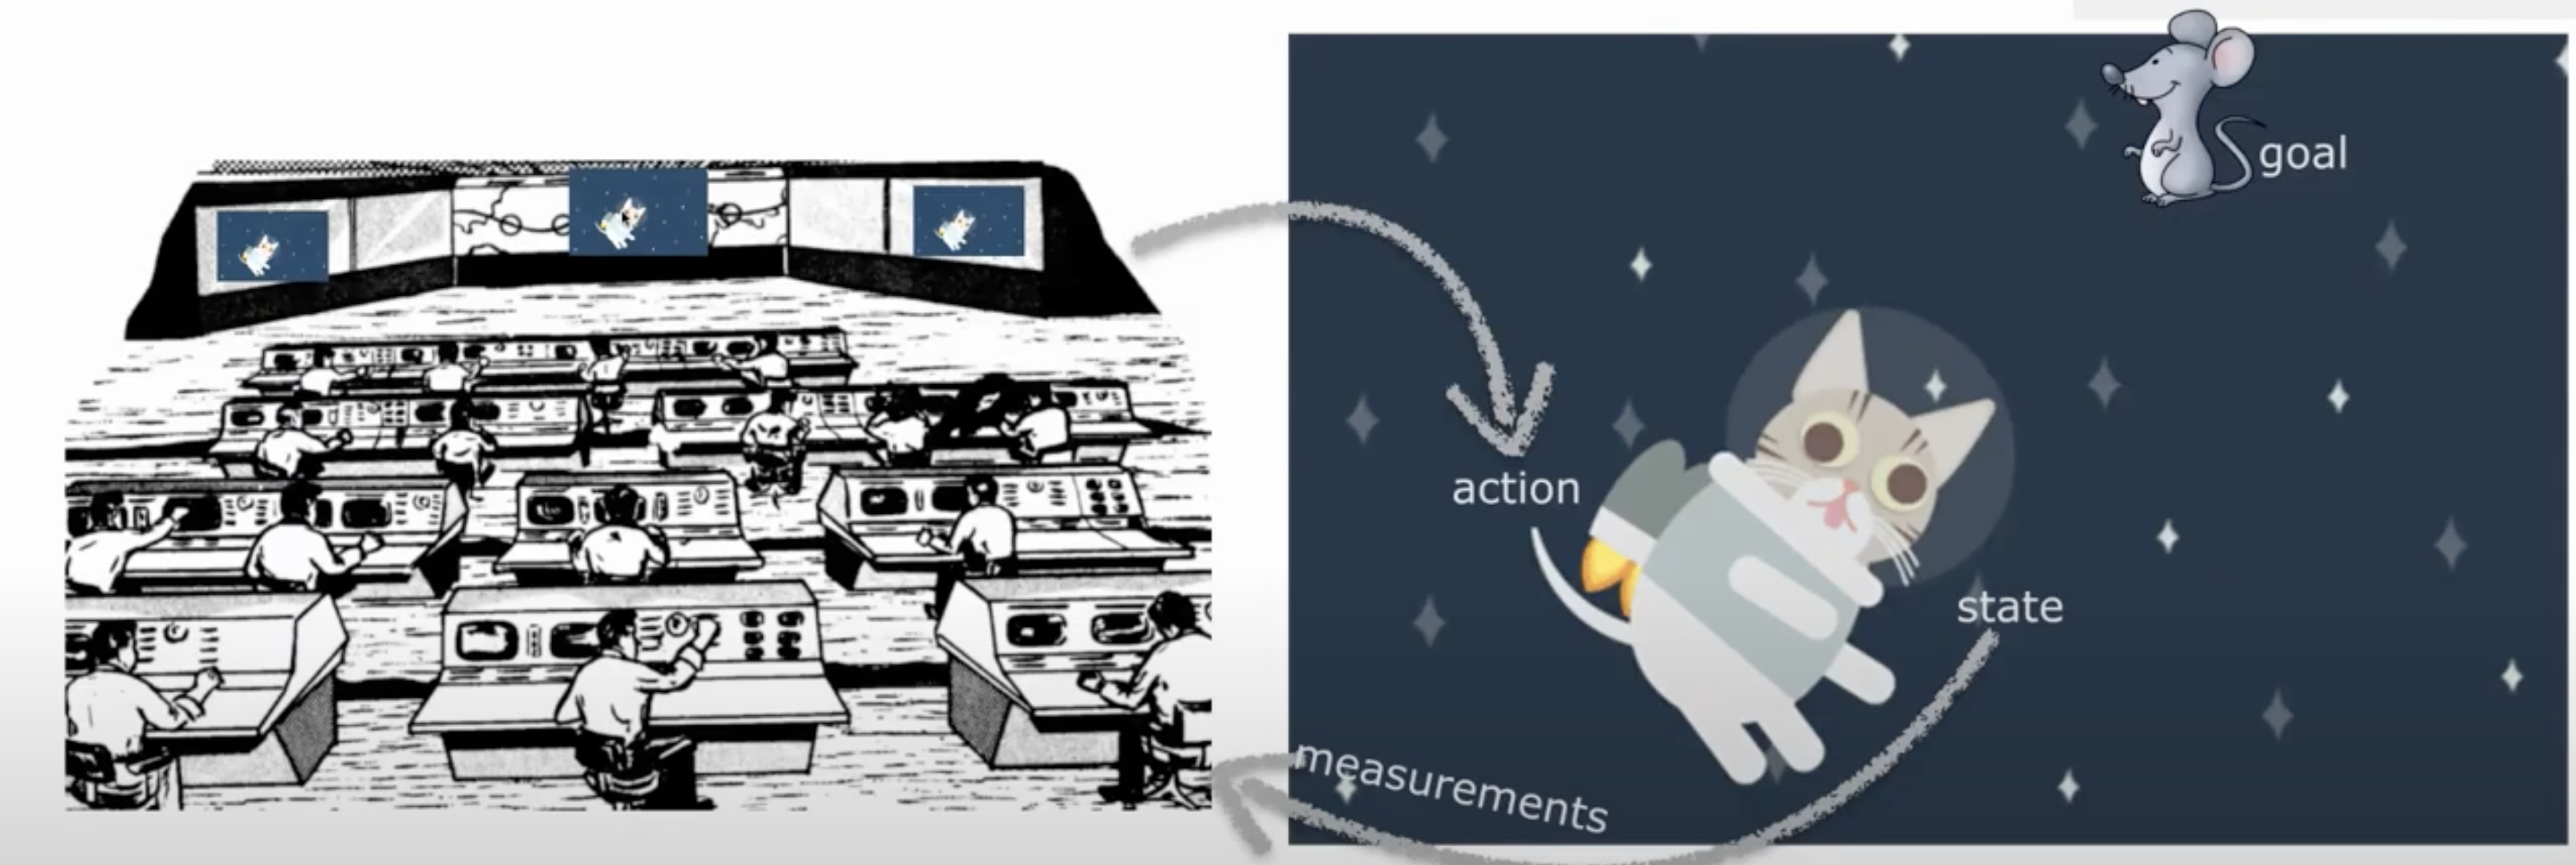
\includegraphics[scale=0.1]{Figures/BD/BD_Figure5.png}
\end{center}


Astrocat is in space and we are considering the position along one dimension. So, the hidden state, s, is the true location. The satellites represent potential loss, and the space mouse, gain. Using indirect measurements, you as ground control, can estimate where Astrocat is or decide where it's likely better to send Astrocat.

Remember, in this example, you can think of yourself as a scientist trying to decide where we believe Astrocat is, how to select a point estimate (single guess of location) based on possible errors, and how to account for the uncertainty we have about the location of the satellite and the space mouse. In fact, this is the kind of problem real scientists working to control remote satellites face! However, we can also think of this as what your brain does when it wants to determine a target to make a movement or hit a tennis ball! A number of classic experiments use this kind of framing to study how *optimal* human decisions or movements are! Some examples are in the further reading document.

\end{subbox}

\begin{subbox}{subbox}{Probability distribution of Astrocat location}
\scriptsize
We are going to think first about how Ground Control should estimate his position. We won't consider measurements yet, just how to represent the uncertainty we might have in general. We are now dealing with a continuous distribution - Astrocat's location can be any real number. In the last tutorial, we were dealing with a discrete distribution - the fish were either on one side or the other. 

So how do we represent the probability of each possible point (an infinite number) where the Astrocat could be? 
The Bayesian approach can be used on any probability distribution. While many variables in the world require representation using complex or unknown (e.g. empirical) distributions, we will be using the Gaussian distributions or extensions of it.

\end{subbox}
\end{textbox}
%%%%%%%%%%%%%%%%%%%%%%%%%%%%%%%%%%%%%%%%%%%%%%%%%%
%%%%%%%%%%%%%%%%%%%%%%%%%%%%%%%%%%%%%%%%%%%%%%%%%%
\begin{textbox}{\href{https://compneuro.neuromatch.io/tutorials/W3D1_BayesianDecisions/student/W3D1_Tutorial2.html}{Bayesian inference and decisions with continuous hidden state (W3D1T2)} }
\begin{subbox}{subbox}{The Gaussian distribution}
\scriptsize
Tne distribution we will use throughout this tutorial is the \textbf{Gaussian distribution}, which is also sometimes called the normal distribution. 

This is a special, and commonly used, distribution for a couple reasons. It is actually the focus of one of the most important theorems in statistics: the Central Limit Theorem. This theorem tells us that if you sum a large number of samples of a variable, that sum is normally distributed \textit{no matter what} the original distribution over a variable was. This is a bit too in-depth for us to get into now but check out links in the Bonus for more information. Additionally, Gaussians have some really nice mathematical properties that permit simple closed-form solutions to several important problems. As we will see later in this tutorial, we can extend Gaussians to be even more flexible and well approximate other distributions using mixtures of Gaussians. In short, the Gaussian is probably the most important continuous distribution to understand and use.

Gaussians have two parameters. The \textbf{mean} $\mu$, which sets the location of its center. Its "scale" or spread is controlled by its \textbf{standard deviation} $\sigma$ or its square, the \textbf{variance} $\sigma^2$. These can be a bit easy to mix up: make sure you are careful about whether you are referring to/using standard deviation or variance.


The equation for a Gaussian distribution on a variable $x$ is:
\begin{equation}
\mathcal{N}(\mu,\sigma^2) = \frac{1}{\sqrt{2\pi\sigma^2}}\exp\left(\frac{-(x-\mu)^2}{2\sigma^2}\right)
\end{equation}

In our example, $x$ is the location of the Astrocat in one direction. $\mathcal{N}(\mu,\sigma^2)$ is a standard notation to refer to a $\mathcal{N}$ormal (Gaussian) distribution. For example, $\mathcal{N}(0, 1)$ denotes a Gaussian distribution with mean 0 and variance 1. 

\end{subbox}

\begin{subbox}{subbox}{Multiplying Gaussians}
\scriptsize
When we multiply Gaussians, we are not multiplying random variables but the actual underlying distributions. If we multiply two Gaussian distributions, with means $\mu_1$ and $\mu_2$ and standard deviations $\sigma_1$ and $\sigma_2$, we get another Gaussian. The Gaussian resulting from the multiplication will have mean $\mu_3$ and standard deviation $\sigma_3$ where:

\begin{align}
\mu_{3} &= a\mu_{1} + (1-a)\mu_{2} \\
\sigma_{3}^{-2} &= \sigma_{1}^{-2} + \sigma_{2}^{-2} \\
a &= \frac{\sigma_{1}^{-2}}{\sigma_{1}^{-2} + \sigma_{2}^{-2}}
\end{align}

This may look confusing but keep in mind that the information in a Gaussian is the inverse of its variance: $\frac{1}{\sigma^2}$. Basically, when multiplying Gaussians, the mean of the resulting Gaussian is a weighted average of the original means, where the weights are proportional to the amount of information of that Gaussian.

\end{subbox}
\end{textbox}
%%%%%%%%%%%%%%%%%%%%%%%%%%%%%%%%%%%%%%%%%%%%%%%%%%
%%%%%%%%%%%%%%%%%%%%%%%%%%%%%%%%%%%%%%%%%%%%%%%%%%
\begin{textbox}{\href{https://compneuro.neuromatch.io/tutorials/W3D1_BayesianDecisions/student/W3D1_Tutorial2.html}{Bayesian inference and decisions with continuous hidden state (W3D1T2)} }
\begin{subbox}{subbox}{Multiplying Gaussians}
\scriptsize

Multiplying two Gaussians, imagine we want to find the middle location between the satellite and the space mouse. This would be the center (average) of the two locations. Because we have uncertainty, we need to weigh our uncertainty in thinking about the most likely place. 


\begin{center}
    
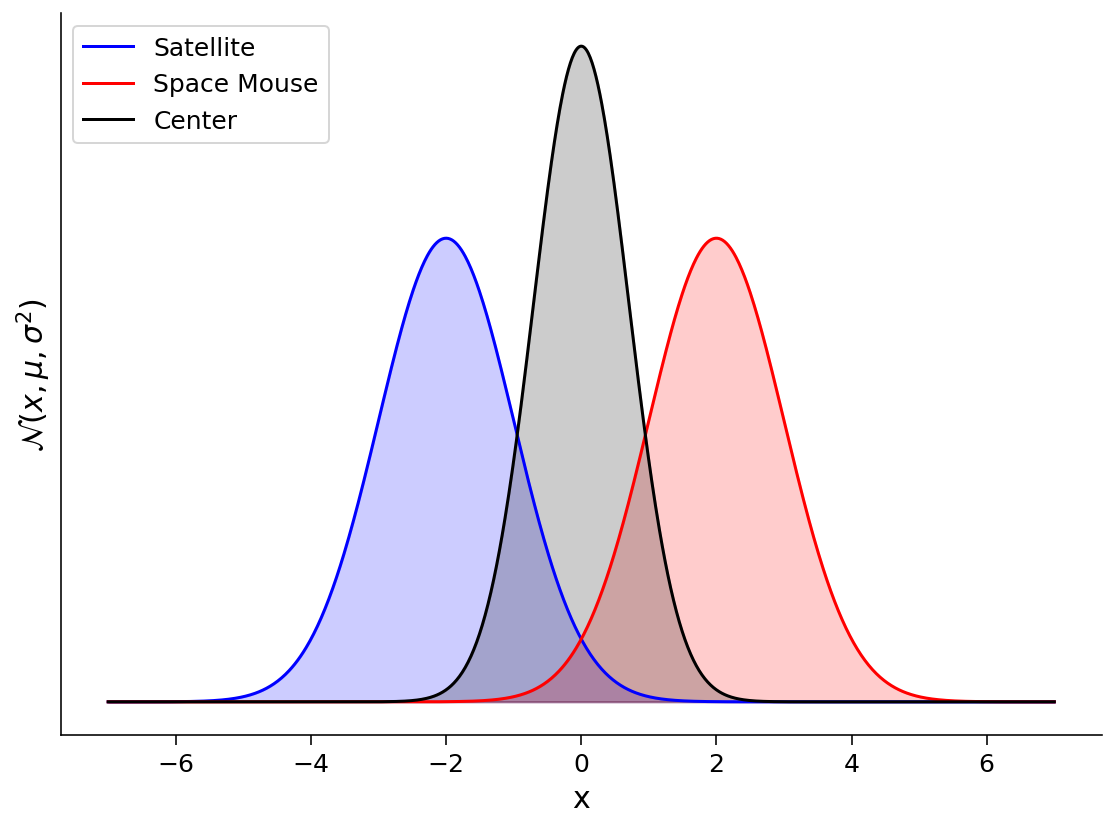
\includegraphics[scale=0.18]{Figures/BD/BD_Figure6.png}
\end{center}
\end{subbox}
\begin{subbox}{subbox}{Mixtures of Gaussians}
\scriptsize

What if our continuous distribution isn't well described by a single bump? For example, what if the Astrocat is often either in one place or another - a Gaussian distribution would not capture this well! We need a multimodal distribution. Luckily, we can extend Gaussians into a \textit{mixture of Gaussians}, which are more complex distributions.  

In a Gaussian mixture distribution, you are essentially adding two or more weighted standard Gaussian distributions (and then normalizing so everything integrates to 1). Each standard Gaussian involved is described, as normal, by its mean and standard deviation. Additional parameters in a mixture of Gaussians are the weights you put on each Gaussian (π). The following demo should help clarify how a mixture of Gaussians relates to the standard Gaussian components. We will not cover the derivation here but you can work it out as a bonus exercise.

Mixture distributions are a common tool in Bayesian modeling and an important tool in general.

We will examining a mixture of two Gaussians. We will have one weighting parameter, $\pi$, that tells us how to weigh one of the Gaussians. The other is weighted by $1 -\pi$. 

\begin{center}
    
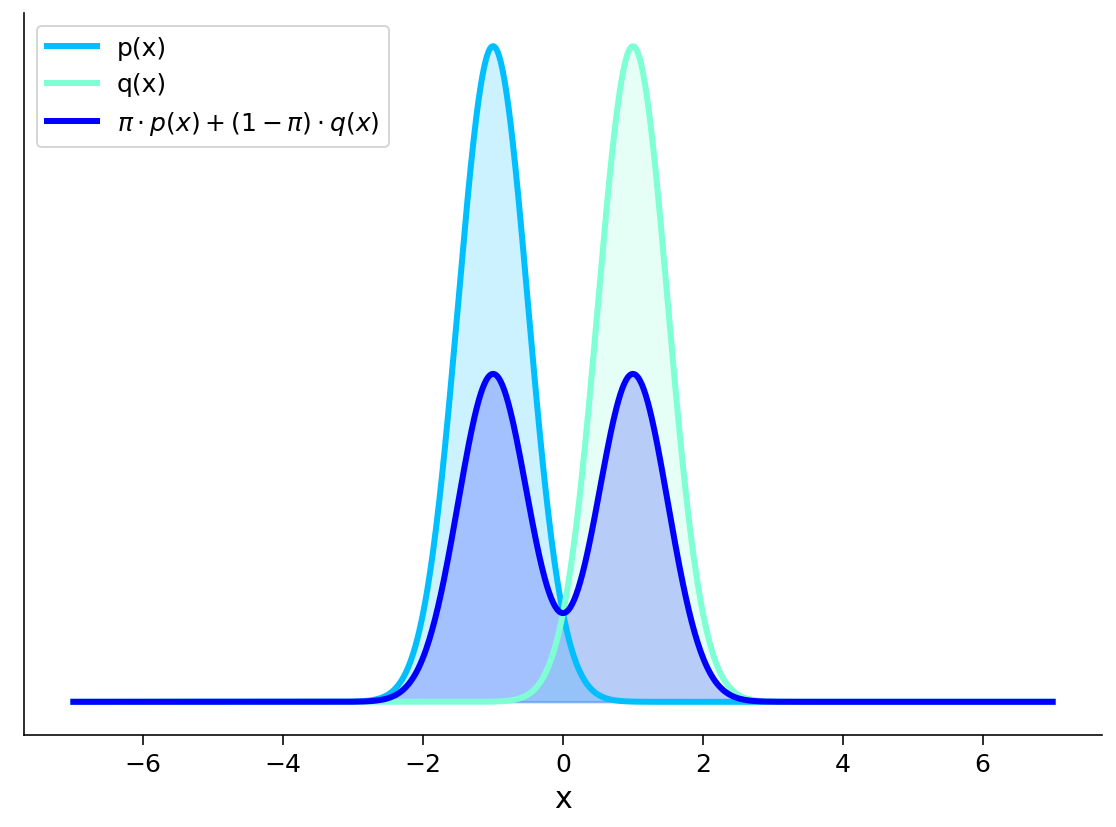
\includegraphics[scale=0.22]{Figures/BD/BD_Figure7.png}
\end{center}
\end{subbox}


\end{textbox}
%%%%%%%%%%%%%%%%%%%%%%%%%%%%%%%%%%%%%%%%%%%%%%%%%%
%%%%%%%%%%%%%%%%%%%%%%%%%%%%%%%%%%%%%%%%%%%%%%%%%%
\begin{textbox}{\href{https://compneuro.neuromatch.io/tutorials/W3D1_BayesianDecisions/student/W3D1_Tutorial2.html}{Bayesian inference and decisions with continuous hidden state (W3D1T2)} }
\begin{subbox}{subbox}{Utility Loss Estimators}
\scriptsize

There are lots of different possible loss functions. We will focus on three: \textbf{mean-squared error} where the loss is the difference between truth and estimate squared, \textbf{absolute error} where the loss is the absolute difference between truth and estimate, and \textbf{Zero-one Loss} where the loss is 1 unless we're exactly right (the estimate equals the truth). We can represent these with the following formulas:

\begin{eqnarray}
\textrm{Mean Squared Error} &=& (\mu - \hat{\mu})^2 \\ 
\textrm{Absolute Error} &=& \big|\mu - \hat{\mu}\big| \\ 
\textrm{Zero-One Loss} &=& \begin{cases}
                            0,& \textrm{if } \mu = \hat{\mu} \\
                            1,              & \textrm{otherwise}
                            \end{cases}
\end{eqnarray}


We will now explore how these different loss functions change our expected utility!

\begin{center}
    
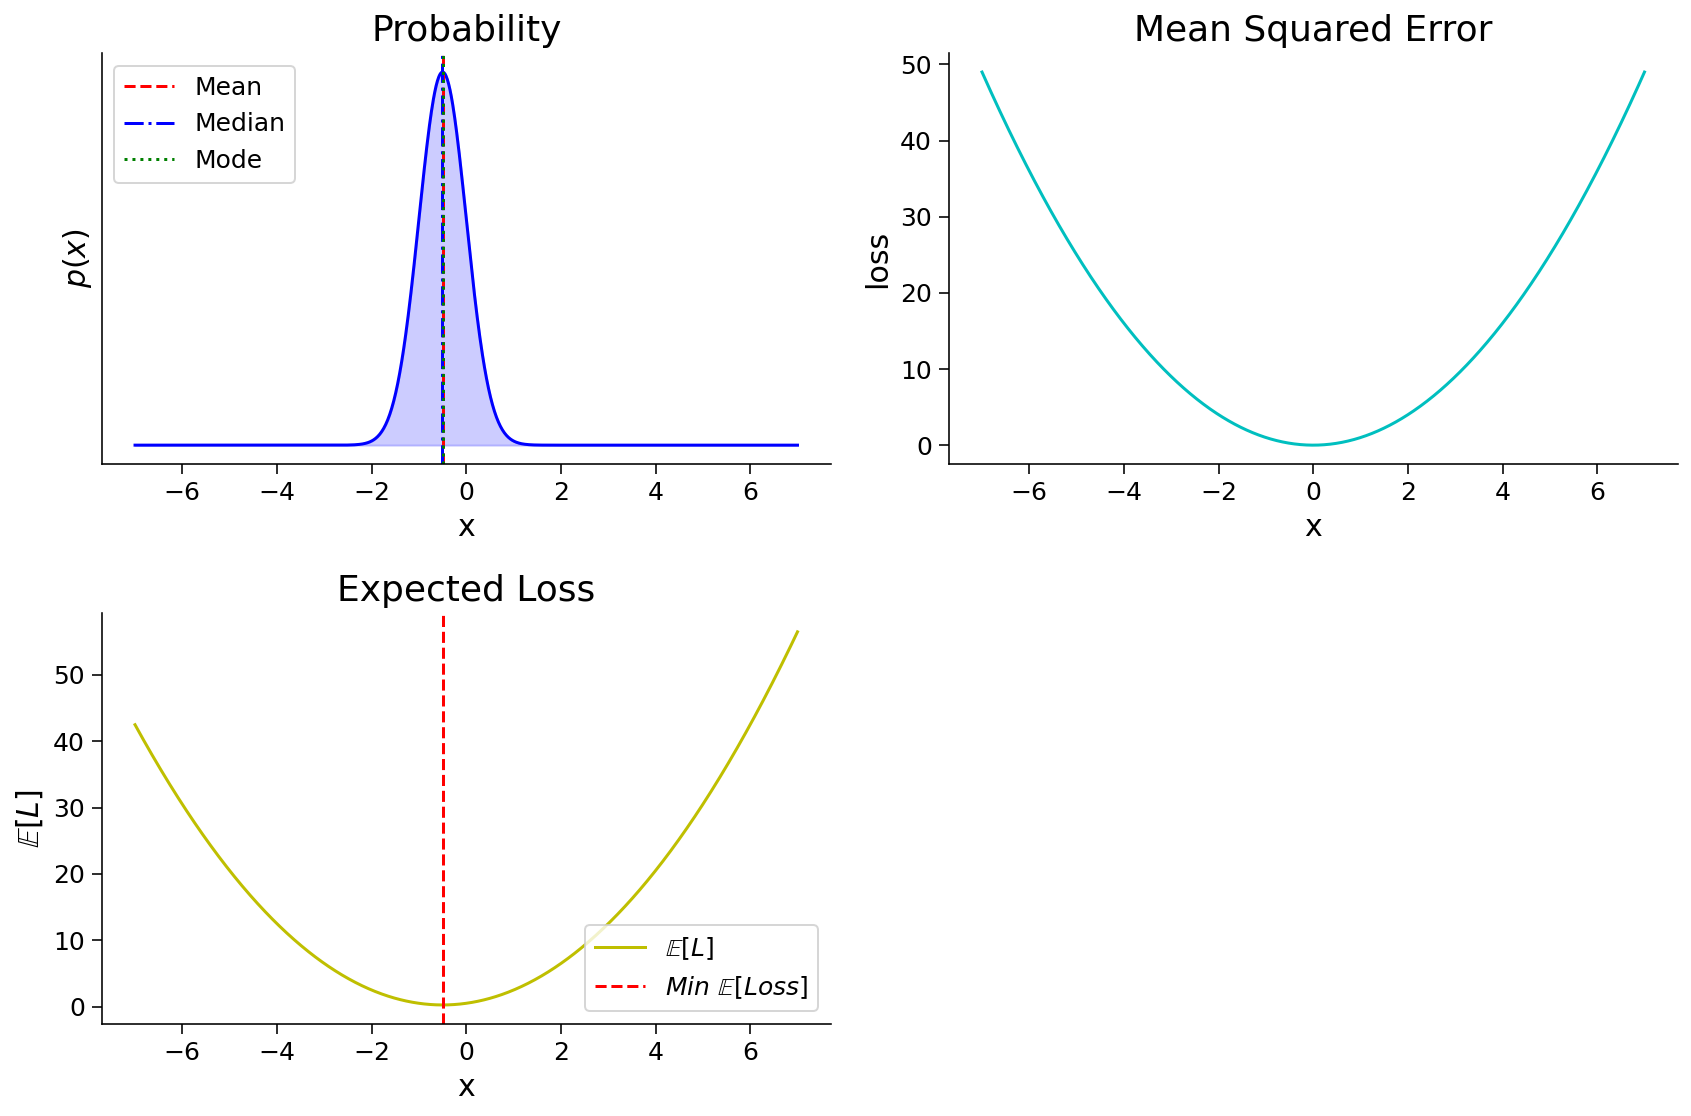
\includegraphics[scale=0.22]{Figures/BD/BD_Figure8.png}
\end{center}

You can see that what coordinates you would provide for Astrocat aren't necessarily easy to guess just from the probability distribution. You need the concept of utility/loss and a specific loss function to determine what estimate you should give.

For symmetric distributions, you will find that the mean, median and mode are the same. However, for distributions with \textit{skew}, like the Gamma distribution or the Exponential distribution, these will be different. You will be able to explore more distributions as priors below.

\end{subbox}

\end{textbox}
%%%%%%%%%%%%%%%%%%%%%%%%%%%%%%%%%%%%%%%%%%%%%%%%%%
%%%%%%%%%%%%%%%%%%%%%%%%%%%%%%%%%%%%%%%%%%%%%%%%%%
\begin{textbox}{\href{https://compneuro.neuromatch.io/tutorials/W3D1_BayesianDecisions/student/W3D1_Tutorial2.html}{Bayesian inference and decisions with continuous hidden state (W3D1T2)} }
\begin{subbox}{subbox}{A more complex loss function}
\scriptsize



The loss functions we just explored were fairly simple and are often used. However, life can be complicated and in this case, Astrocat cares about both being near the space mouse and avoiding the satellites. This means we need a more complex loss function that captures this! 

We know that we want to estimate Astrocat to be closer to the mouse, which is safe and desirable, but further away from the satellites, which is dangerous! So, rather than thinking about the *Loss* function, we will consider a generalized utility function that considers gains and losses that \textit{matter} to Astrocat!
\begin{center}
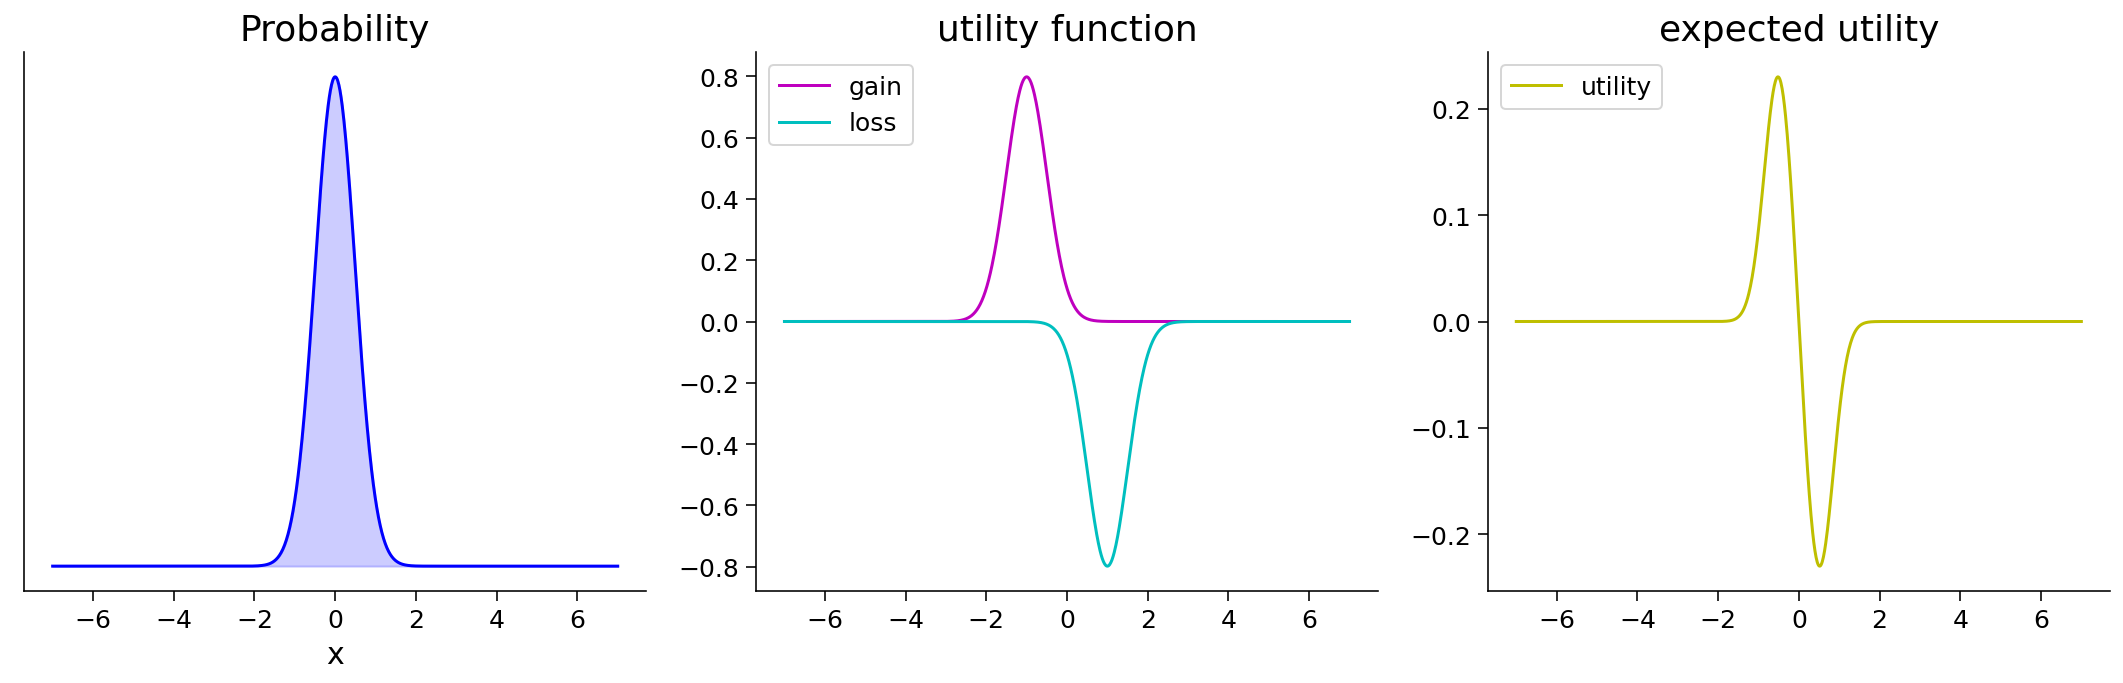
\includegraphics[scale=0.18]{Figures/BD/BD_Figure9.png}
\end{center}


\end{subbox}
\begin{subbox}{subbox}{Correlation and marginalization}
\scriptsize

If the two variables in a two dimensional Gaussian are independent, looking at one tells us nothing about the other. But what if the the two variables are correlated (covary)?

The covariance of two Gaussians with means $\mu_X$ and $\mu_Y$ and standard deviations $\sigma_X$ and $\sigma_Y$is:

\begin{equation}
\sigma_{XY} = \mathbb{E}[(X-\mu_{X})(Y-\mu_{Y})]
\end{equation}

$\mathbb{E}[\cdot]$ here denotes the expected value. So the covariance is the expected value of the random variable $X$ minus the mean of the Gaussian distribution on $X$ times the random variable Y minus the mean of the Gaussian distribution on $Y$.

The correlation is the covariance normalized, so that it goes between -1 (exactly anticorrelated) to 1 (exactly correlated).

\begin{equation}
\rho_{XY} = \frac{\sigma_{XY}}{\sigma_{X}\sigma_{Y}}
\end{equation}

These are key concepts and while we are considering two hidden states (or two random variables), they extend to $N$ dimensional vectors of Gaussian random variables. You will find these used all over computational neuroscience.
\begin{center}
    
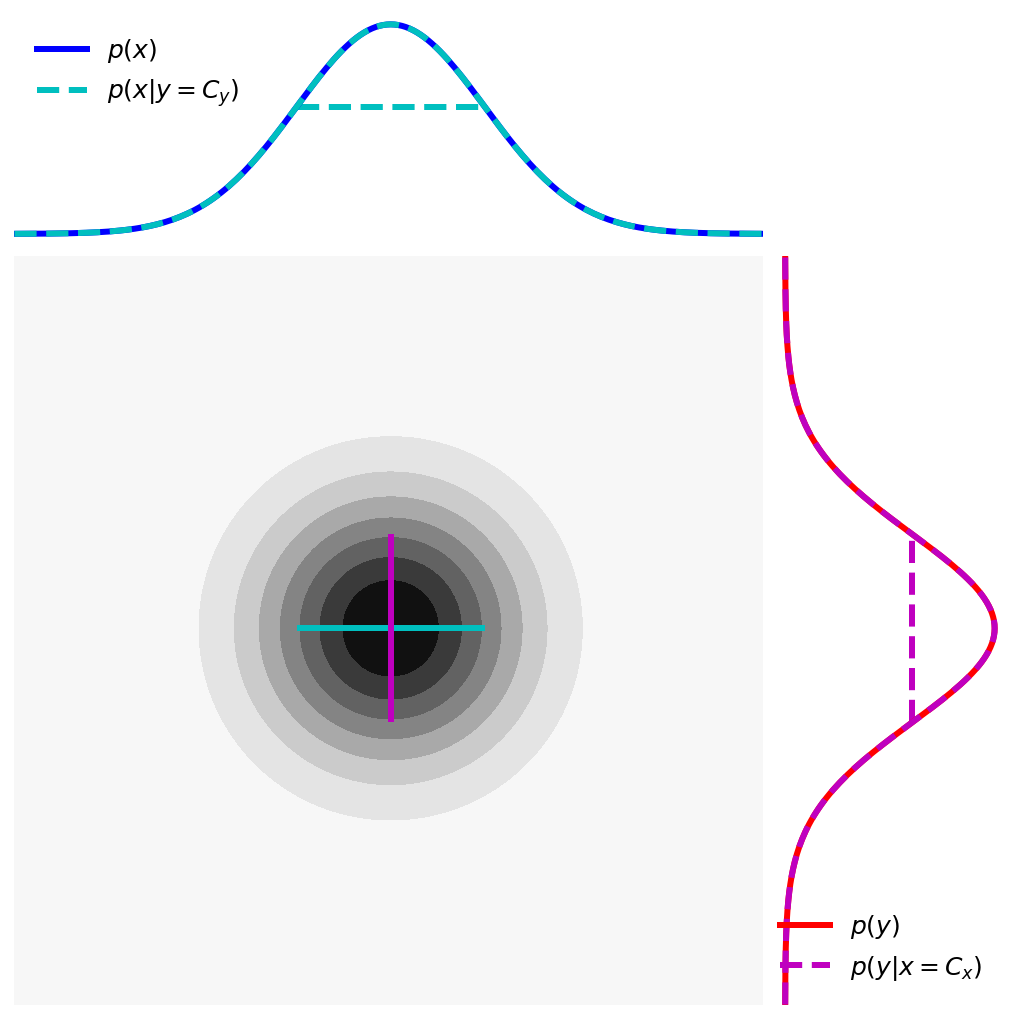
\includegraphics[scale=0.18]{Figures/BD/BD_Figure10.png}
\end{center}

\end{subbox}
\end{textbox}
%%%%%%%%%%%%%%%%%%%%%%%%%%%%%%%%%%%%%%%%%%%%%%%%%%
%%%%%%%%%%%%%%%%%%%%%%%%%%%%%%%%%%%%%%%%%%%%%%%%%%
\begin{textbox}{\href{https://compneuro.neuromatch.io/tutorials/W3D1_BayesianDecisions/student/W3D1_Tutorial2.html}{Bayesian inference and decisions with continuous hidden state (W3D1T2)} }
\begin{subbox}{subbox}{Bayes' theorem for continuous distributions}
\scriptsize

The continuous case allows us to consider how the shape of the posterior distribution can differ from the prior. The Gaussian case is the most fundamental, but asymmetric priors (or likelihoods) and posteriors allow us to see how the mean, median and mode can be affected differently when we apply Bayes' theorem.

\end{subbox}
\begin{subbox}{subbox}{The Gaussian example}
\scriptsize
Bayes' rule tells us how to combine two sources of information: the prior (e.g., a noisy representation of Ground Control's expectations about where Astrocat is) and the likelihood (e.g., a noisy representation of the Astrocat after taking a measurement), to obtain a posterior distribution (our belief distribution) taking into account both pieces of information. Remember Bayes' rule:

\begin{equation}
\text{Posterior} = \frac{ \text{Likelihood} \times \text{Prior}}{ \text{Normalization constant}}
\end{equation}

We will look at what happens when both the prior and likelihood are Gaussians. In these equations, $\mathcal{N}(\mu,\sigma^2)$ denotes a Gaussian distribution with parameters $\mu$ and $\sigma^2$:

\begin{equation}
\mathcal{N}(\mu, \sigma) = \frac{1}{\sqrt{2 \pi \sigma^2}} \; \exp \bigg( \frac{-(x-\mu)^2}{2\sigma^2} \bigg)
\end{equation}

When both the prior and likelihood are Gaussians, Bayes Rule translates into the following form:
\tiny
\begin{align*}
\text{Likelihood} &= \mathcal{N}(\mu_{likelihood},\sigma_{likelihood}^2) \\
\text{Prior} &= \mathcal{N}(\mu_{prior},\sigma_{prior}^2) \\
\text{Posterior} &= \mathcal{N}\left( \frac{\sigma^2_{likelihood}\mu_{prior}+\sigma^2_{prior}\mu_{likelihood}}{\sigma^2_{likelihood}+\sigma^2_{prior}},\right.\\
& \left. \frac{\sigma^2_{likelihood}\sigma^2_{prior}}{\sigma^2_{likelihood}+\sigma^2_{prior}} \right) \\
&\propto \mathcal{N}(\mu_{likelihood},\sigma_{likelihood}^2) \times \mathcal{N}(\mu_{prior},\sigma_{prior}^2)
\end{align*}


\begin{center}
    
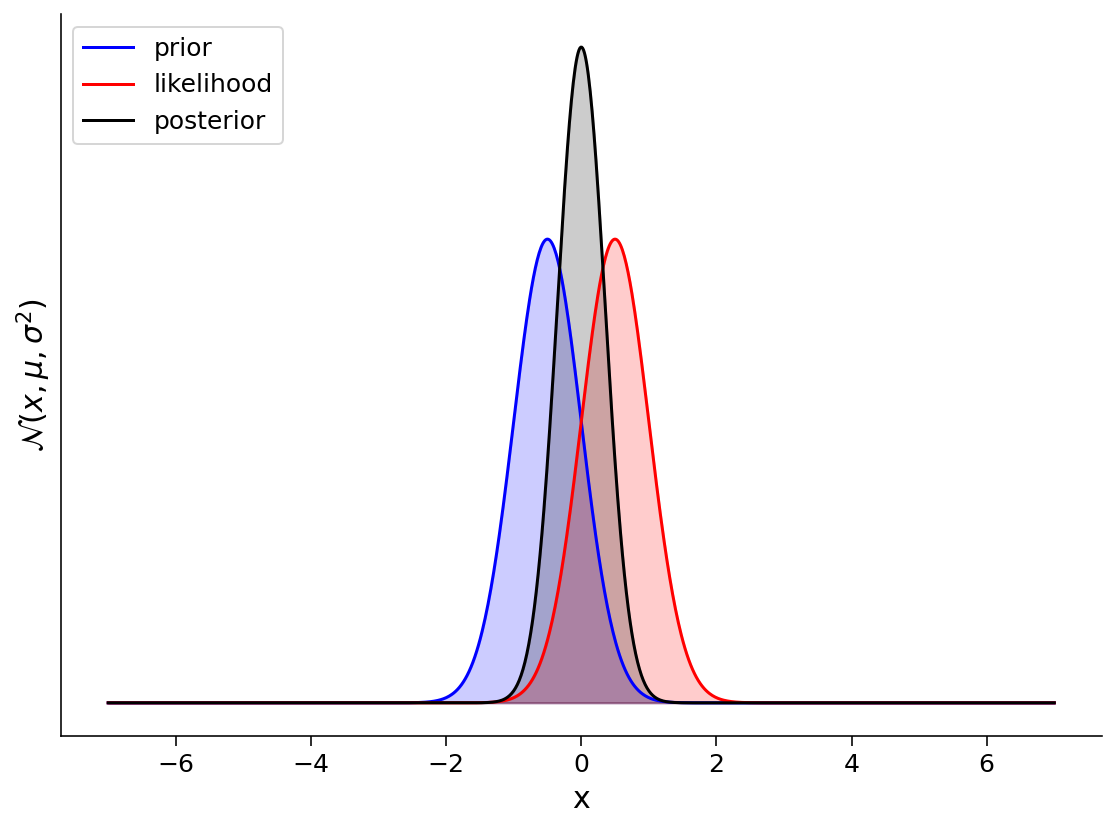
\includegraphics[scale=0.23]{Figures/BD/BD_Figure11.png}
\end{center}

\end{subbox}
\end{textbox}
%%%%%%%%%%%%%%%%%%%%%%%%%%%%%%%%%%%%%%%%%%%%%%%%%%
%%%%%%%%%%%%%%%%%%%%%%%%%%%%%%%%%%%%%%%%%%%%%%%%%%
\begin{textbox}{\href{https://compneuro.neuromatch.io/tutorials/W3D1_BayesianDecisions/student/W3D1_Tutorial2.html}{Bayesian inference and decisions with continuous hidden state (W3D1T2)} }
\begin{subbox}{subbox}{Bayesian estimation on the posterior}
\scriptsize


Bayesian decisions in continuous dimensions are the same as for the binary case. The only difference is that now, our Expected Utility is calculated using an integral and all of our probability distributions are continuous.
\begin{center}
    
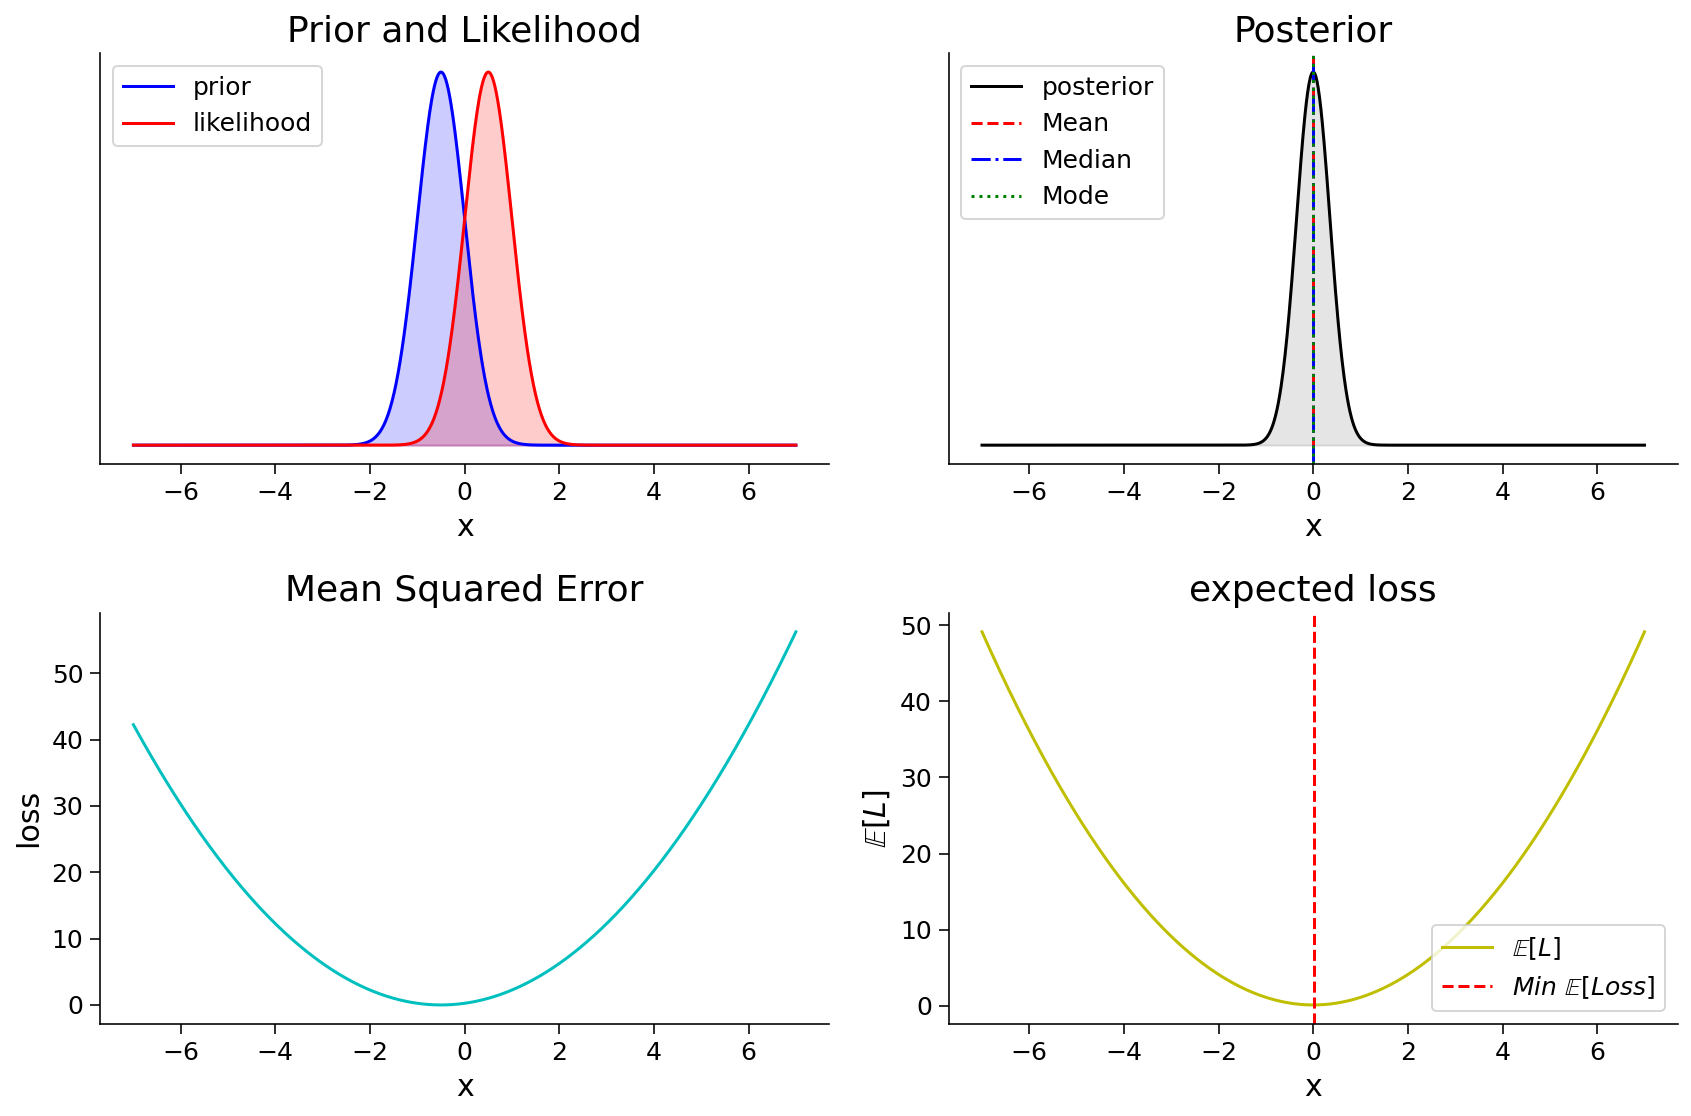
\includegraphics[scale=0.23]{Figures/BD/BD_Figure12.png}
\end{center}
\end{subbox}
\begin{subbox}{subbox}{Bayesian decisions}
\scriptsize
Finally, we can combine everything we have learned so far! 

Now, let's imagine we have just received a new measurement of Astrocat's location. We need to think about how we want to decide where Astrocat is, so that we can decide how far to tell Astrocat to move. However, we want to account for the satellite and Space Mouse location in this estimation. If we make an error towards the satellite, it's worse than towards Space Mouse. So, we will use our more complex utility function than before. 

\begin{center}
    
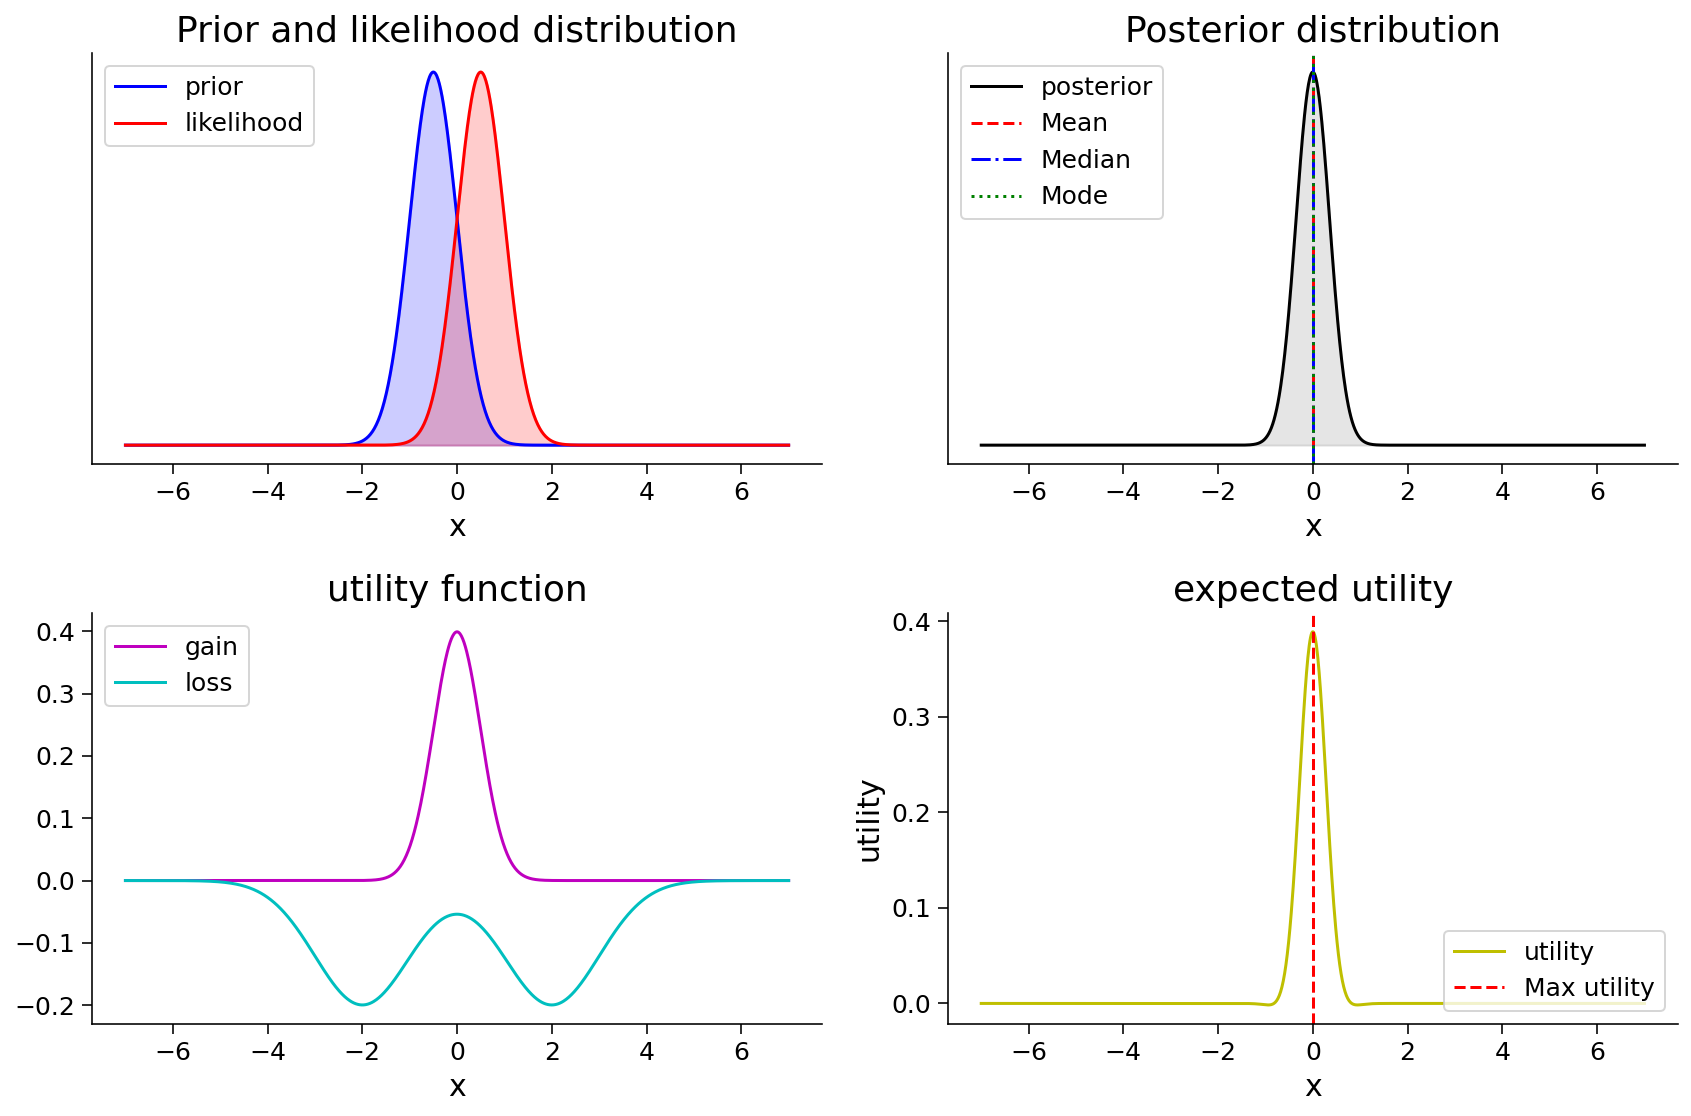
\includegraphics[scale=0.23]{Figures/BD/BD_Figure13.png}
\end{center}

\end{subbox}
\end{textbox}


\end{multicols}
\newpage
%%% Hidden Dynamics
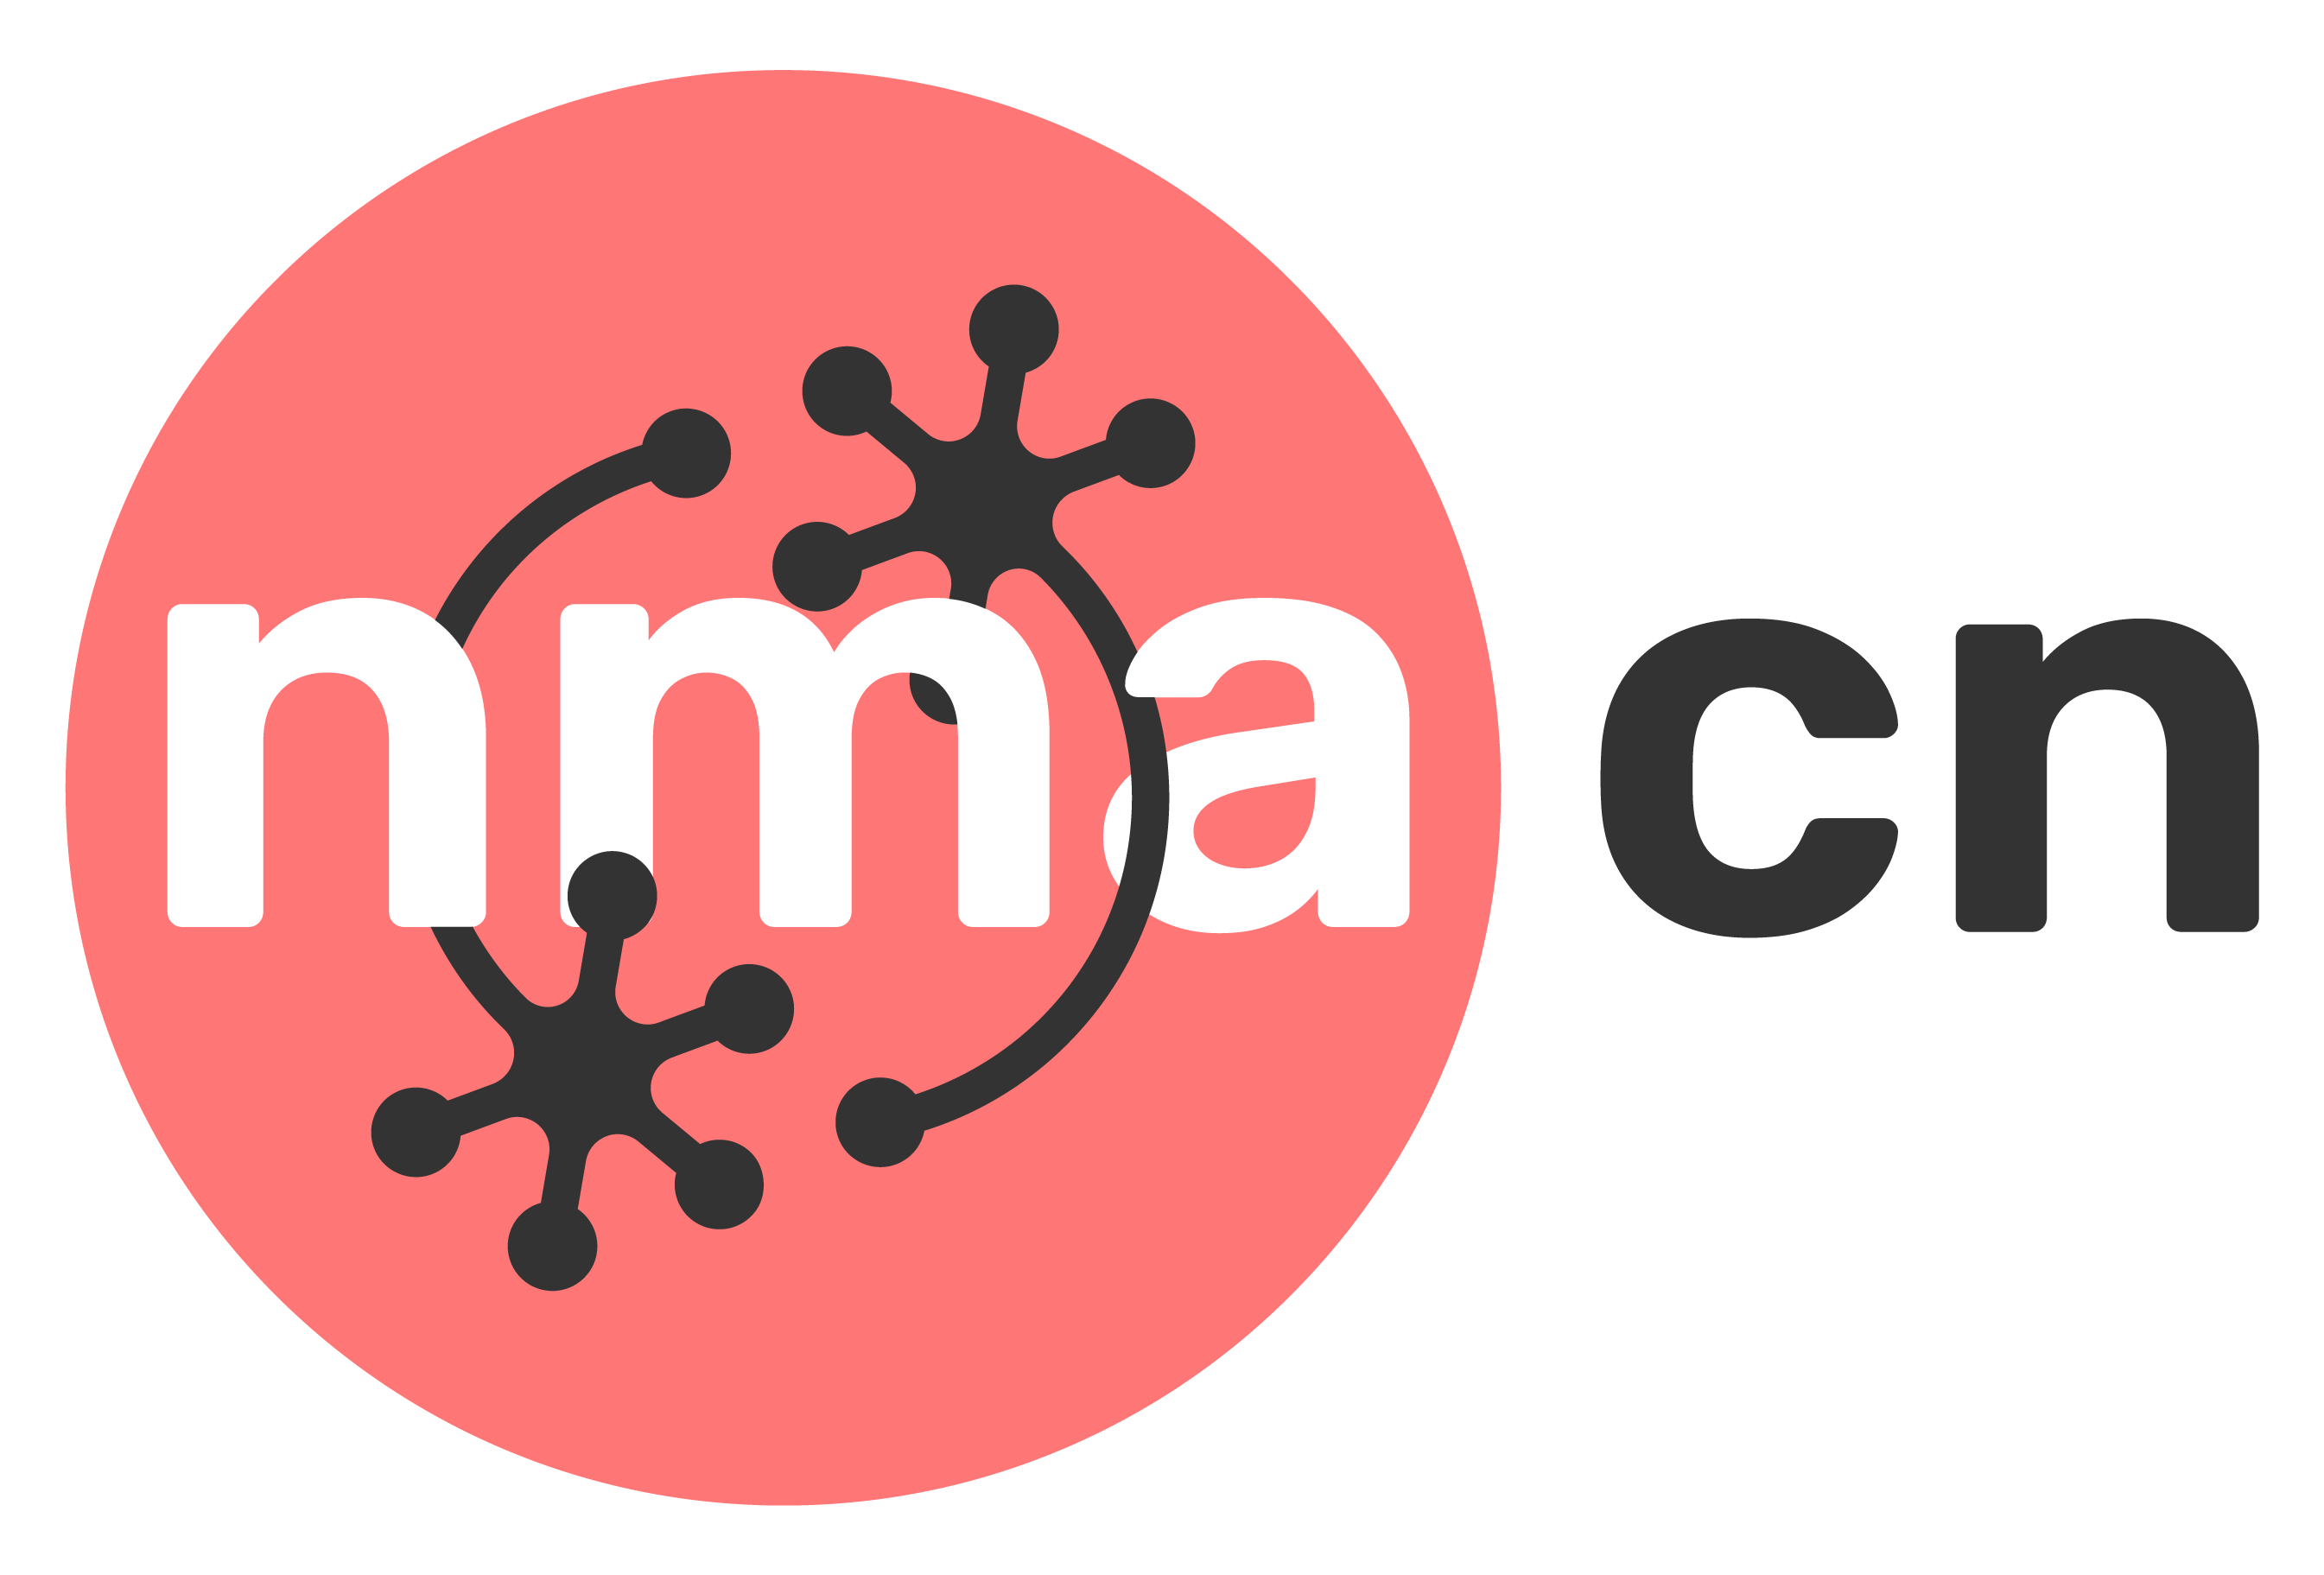
\includegraphics[scale=0.03]{Figures/NMACN.png}\href{https://compneuro.neuromatch.io/tutorials/intro.html}{\textbf{\Huge{Neuromatch Academy: Hidden Dynamics - Summary Sheet}}\footnote{’t Hart et al., (2022). Neuromatch Academy: a 3-week, online summer school in computational neuroscience. Journal of Open Source Education, 5(49), 118. https://doi.org/10.21105/jose.00118}}
%$\subsection*{Cheat Sheet}
\small
\begin{multicols}{3}

\let\clearpage\relax
\begin{textbox}{\href{https://compneuro.neuromatch.io/tutorials/W3D2_HiddenDynamics/student/W3D2_Tutorial1.html}{Sequential Probability Ratio Test (W3D2T1)}   }
\begin{subbox}{subbox}{Overview}
\scriptsize
Here we will learn about Hidden Markov Models (HMMs), which allow us to infer things in the world from a stream of data. For the binary case, we start with a simple version where the latent state doesn’t change, then we’ll allow the latent state to change over time. The core learning objective is to understand and implement an algorithm to infer a changing hidden state from observations.

The HMM combines ideas from the linear dynamics lessons (which used Markov models) with inferences described in the Bayes day (which used Hidden variables). It also connects directly to later lessons in Optimal Control and Reinforcement Learning, which often use the HMM to guide actions.

The HMM is a pervasive model in neuroscience. It is used for data analysis, like inferring neural activity from fluorescence images. It is also a foundational model for what the brain should compute, as it interprets the physical world that is observed only through its senses.

Bayes' Theorem combines the sensory measurement $m$ about a latent variable $s$ with our prior knowledge. This produced a posterior probability distribution $p(s|m)$. Here we will allow for dynamic world states and measurements.

 We will assume that the world state is binary ($\pm 1$) and constant over time, but allow for multiple observations over time. We will use the \textbf{Sequential Probability Ratio Test (SPRT)} to infer which state is true. This leads to the \textbf{Drift Diffusion Model (DDM)} where evidence accumulates until reaching a stopping criterion.

\end{subbox}



\end{textbox}
%%%%%%%%%%%%%%%%%%%%%%%%% 
%%%%%%%%%%%%%%%%%%%%%%%%%
\begin{textbox}{\href{https://compneuro.neuromatch.io/tutorials/W3D2_HiddenDynamics/student/W3D2_Tutorial1.html}{Sequential Probability Ratio Test (W3D2T1)}   }


\begin{subbox}{subbox}{Sequential Probability Ratio Test as a Drift Diffusion Model}
\scriptsize
The Sequential Probability Ratio Test is a likelihood ratio test for determining which of two hypotheses is more likely. It is appropriate for sequential independent and identically distributed (iid) data. iid means that the data comes from the same distribution.

Let's return to what we learned yesterday. We had probabilities of our measurement ($m$) given a state of the world ($s$). For example, we knew the probability of seeing someone catch a fish while fishing on the left side given that the fish were on the left side $P(m = \textrm{catch fish} | s = \textrm{left})$.

Now let's extend this slightly to assume we take a series of measurements, from time 1 up to time t ($m_{1:t}$), and that our state is either +1 or -1. We want to figure out what the state is, given our measurements. To do this, we can compare the total evidence up to time $t$ for our two hypotheses (that the state is +1 or that the state is -1). We do this by computing a likelihood ratio: the ratio of the likelihood of all these measurements given the state is +1, $p(m_{1:t}|s=+1)$, to the likelihood of the measurements given the state is -1, $p(m_{1:t}|s=-1)$. This is our likelihood ratio test. In fact, we want to take the log of this likelihood ratio to give us the log likelihood ratio $L_T$.

\begin{align*}
L_T &= log\frac{p(m_{1:t}|s=+1)}{p(m_{1:t}|s=-1)}
\end{align*}

Since our data is independent and identically distribution, the probability of all measurements given the state equals the product of the separate probabilities of each measurement given the state ($p(m_{1:t}|s) = \prod_{t=1}^T p(m_t | s) $). We can substitute this in and use log properties to convert to a sum.

\begin{align*}
L_T &= log\frac{p(m_{1:t}|s=+1)}{p(m_{1:t}|s=-1)}\\
&= log\frac{\prod_{t=1}^Tp(m_{t}|s=+1)}{\prod_{t=1}^Tp(m_{t}|s=-1)}\\
&= \sum_{t=1}^T log\frac{p(m_{t}|s=+1)}{p(m_{t}|s=-1)}\\
&= \sum_{t=1}^T \Delta_t
\end{align*}

In the last line, we have used $\Delta_t = log\frac{p(m_{t}|s=+1)}{p(m_{t}|s=-1)}$. 
\end{subbox}



\end{textbox}
%%%%%%%%%%%%%%%%%%%%%%%%% 
%%%%%%%%%%%%%%%%%%%%%%%%%
\begin{textbox}{\href{https://compneuro.neuromatch.io/tutorials/W3D2_HiddenDynamics/student/W3D2_Tutorial1.html}{Sequential Probability Ratio Test (W3D2T1)}   }

\begin{subbox}{subbox}{Sequential Probability Ratio Test as a Drift Diffusion Model}
\scriptsize
To get the full log likelihood ratio, we are summing up the log likelihood ratios at each time step. The log likelihood ratio at a time step ($L_T$) will equal the ratio at the previous time step ($L_{T-1}$) plus the ratio for the measurement at that time step, given by $\Delta_T$:

\begin{align*}
L_T =  L_{T-1} + \Delta_T
\end{align*}

The SPRT states that if $L_T$ is positive, then the state $s=+1$ is more likely than $s=-1$! 

\end{subbox}

\begin{subbox}{subbox}{Sequential Probability Ratio Test}
\scriptsize
Let's assume that the probability of seeing a measurement given the state is a Gaussian (Normal) distribution where the mean ($\mu$) is different for the two states but the standard deviation ($\sigma$) is the same:
\begin{align*}
p(m_t | s = +1) &= \mathcal{N}(\mu, \sigma^2)\\
p(m_t | s = -1) &= \mathcal{N}(-\mu, \sigma^2)\\
\end{align*}
We can write the new evidence (the log likelihood ratio for the measurement at time $t$) as
$$\Delta_t=b+c\epsilon_t$$
The first term, $b$, is a consistant value and equals $b=2\mu^2/\sigma^2$. This term favors the actual hidden state. The second term, $c\epsilon_t$ where $\epsilon_t\sim\mathcal{N}(0,1)$, is a standard random variable which is scaled by the diffusion $c=2\mu/\sigma$. You can work through proving this in the bonus exercise 0 below if you wish!

The accumulation of evidence will thus "drift" toward one outcome, while "diffusing" in random directions, hence the term "drift-diffusion model" (DDM). The process is most likely (but not guaranteed) to reach the correct outcome eventually.

Adding these $\Delta_t$ over time gives

\begin{equation*}
L_T\sim\mathcal{N}\left(2\frac{\mu^2}{\sigma^2}T,\ 4\frac{\mu^2}{\sigma^2}T\right)=\mathcal{N}(bT,c^2T)
\end{equation*}

as claimed. The log-likelihood ratio $L_t$ is a biased random walk --- normally distributed with a time-dependent mean and variance. This is the \textbf{Drift Diffusion Model}.

\end{subbox}
\end{textbox}
%%%%%%%%%%%%%%%%%%%%%%%%% 
%%%%%%%%%%%%%%%%%%%%%%%%%
\begin{textbox}{\href{https://compneuro.neuromatch.io/tutorials/W3D2_HiddenDynamics/student/W3D2_Tutorial1.html}{Sequential Probability Ratio Test (W3D2T1)}   }

\begin{subbox}{subbox}{Plotting an SPRT model}
\scriptsize


Let's now generate simulated data with $s=+1$ and see if the SPRT can infer the state correctly.

The plot below visualizes 10 simulations of the DDM.
\begin{center}
    
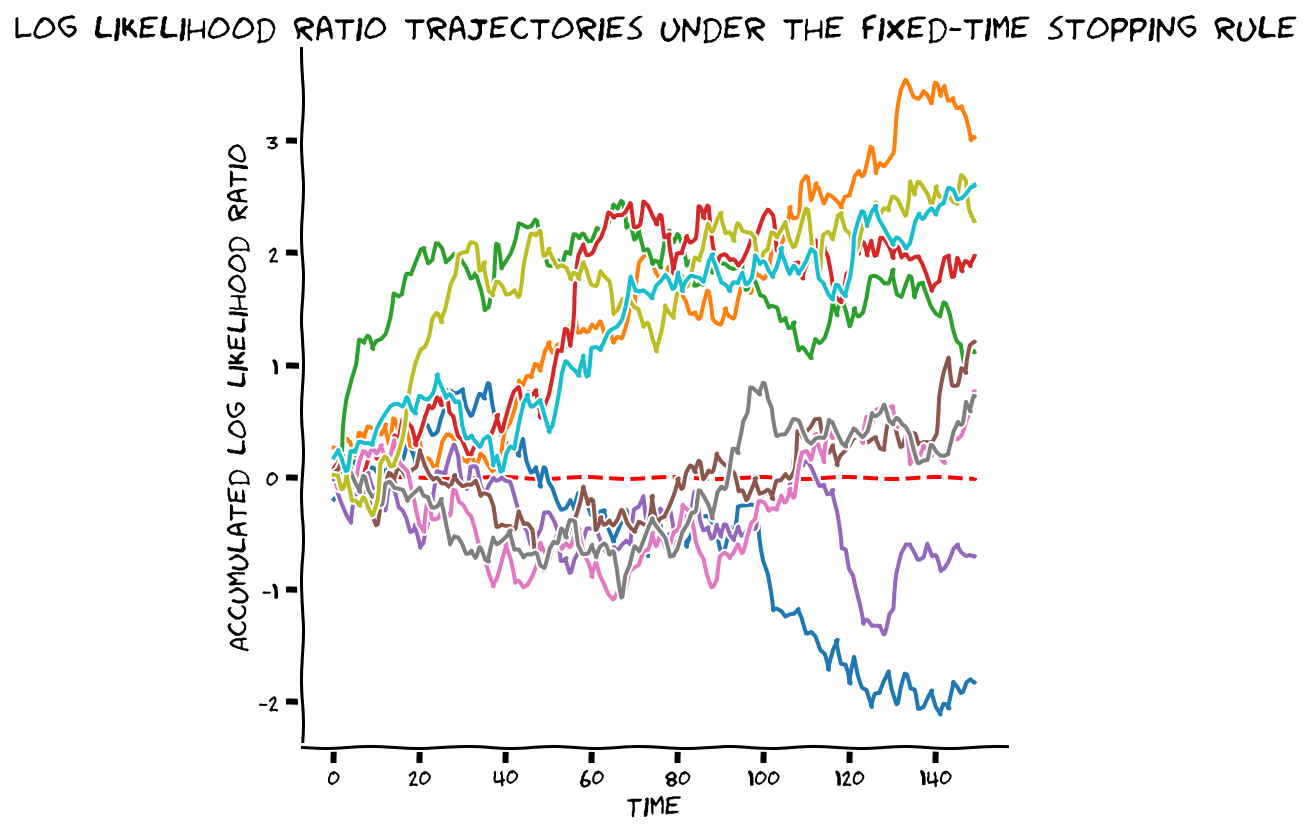
\includegraphics[scale=0.25]{Figures/HD/HD_Figure1.png}
\end{center}
Note:
\begin{enumerate}
    \item 
Higher noise, or higher sigma ($\sigma$), means that the evidence accumulation varies up
   and down more. You are more likely to make a wrong decision with high noise,
   since the accumulated log likelihood ratio is more likely to be negative at the end
   despite the true distribution being s = +1.

\item When sigma ($\sigma$) is very small, the cumulated log likelihood ratios are basically a linear
   diagonal line. This is because each new measurement will be very similar (since they are
   being drawn from a Gaussian with a tiny standard deviation)

\item You are more likely to be wrong with a small number of time steps before decision. There is
   more change that the noise will affect the decision. We will explore this in the next section.
\end{enumerate}

\end{subbox}
\end{textbox}
%%%%%%%%%%%%%%%%%%%%%%%%% 
%%%%%%%%%%%%%%%%%%%%%%%%%
\begin{textbox}{\href{https://compneuro.neuromatch.io/tutorials/W3D2_HiddenDynamics/student/W3D2_Tutorial1.html}{Sequential Probability Ratio Test (W3D2T1)}   }

\begin{subbox}{subbox}{Analyzing the DDM: accuracy vs stopping time}
\scriptsize

If you make a hasty decision (e.g., after only seeing 2 samples), or if observation noise buries the signal, you may see a negative accumulated log likelihood ratio and thus make a wrong decision. Let's plot how decision accuracy varies with the number of samples. Accuracy is the proportion of correct trials across our repeated simulations: $\frac{\# \textrm{ correct decisions}}{\# \textrm{ total decisions}}$.

\begin{center}
    
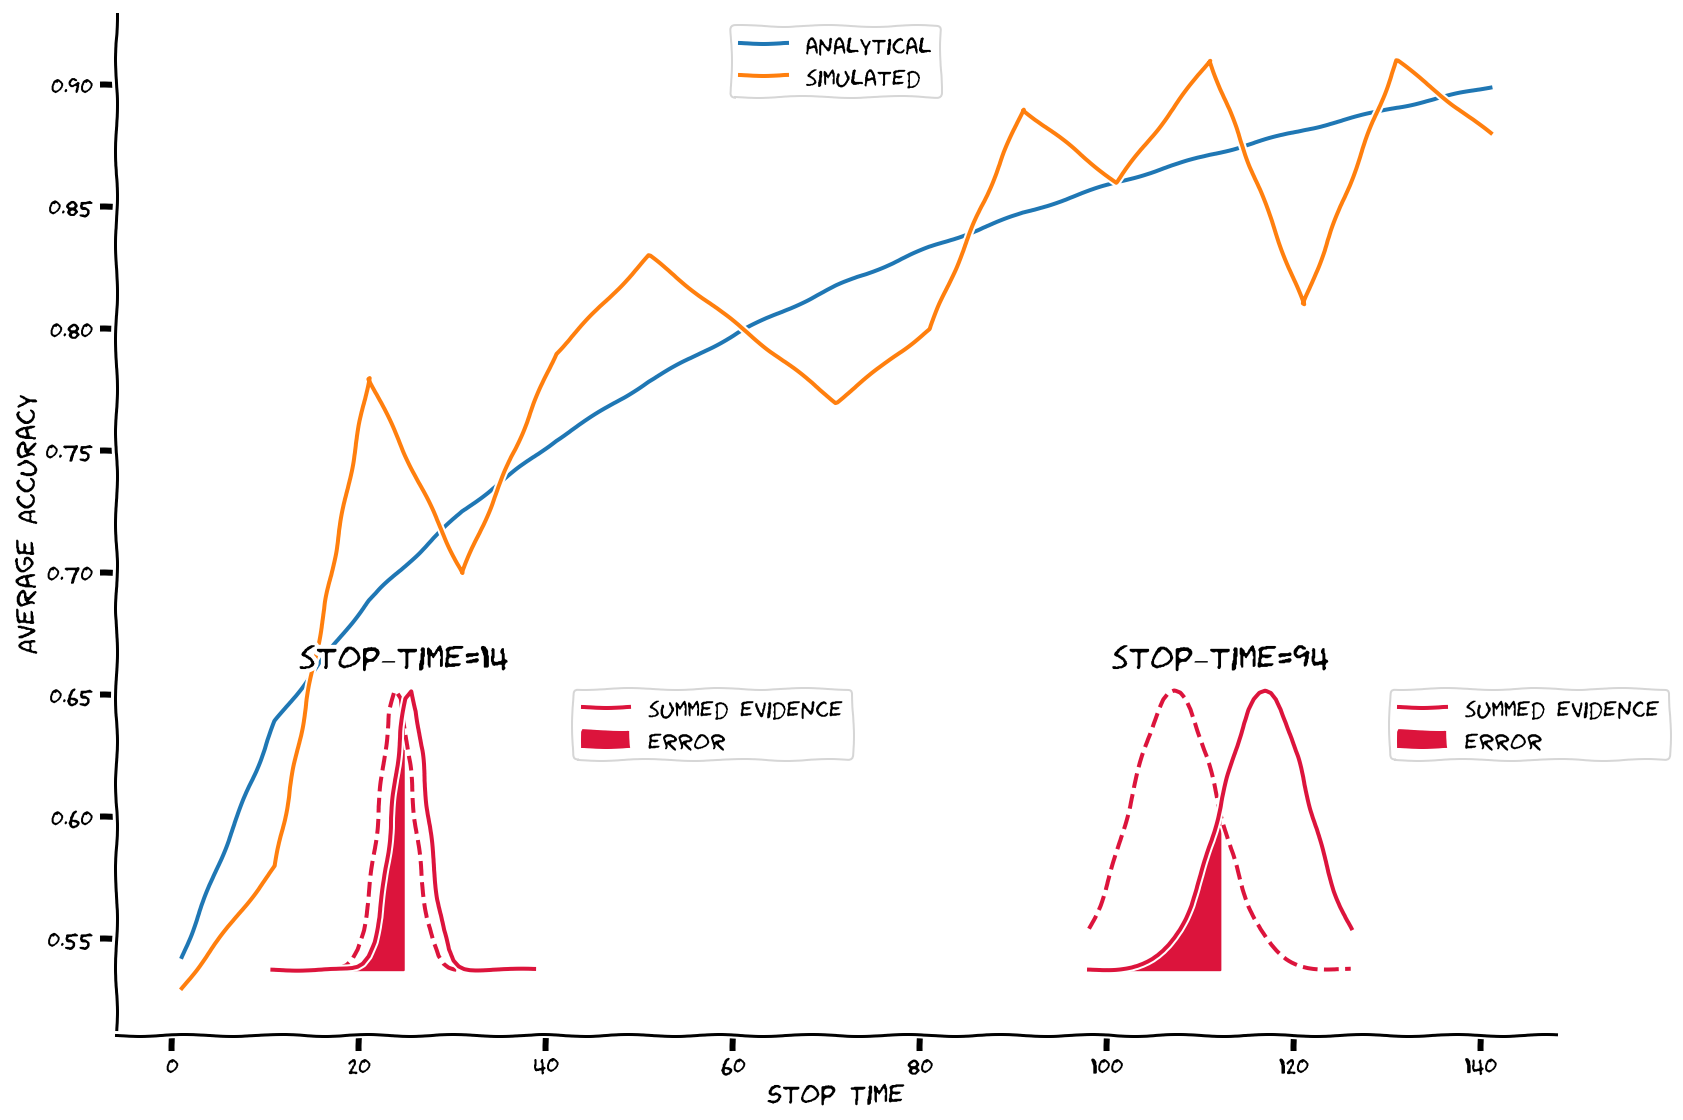
\includegraphics[scale=0.2]{Figures/HD/HD_Figure2.png}
\end{center}
In the figure above, we are plotting the simulated accuracies in orange. We can actually find an analytical equation for the average accuracy in this specific case, which we plot in blue. We will not dive into this analytical solution here but you can imagine that if you ran a bunch of different simulations and had the equivalent number of orange lines, the average of those would resemble the blue line. 

In the insets, we are showing the evidence distributions for the two states at a certain time point. Recall from Section 1 that the likelihood ratio at time $T$ for state of +1 is: 

\begin{equation}
L_T\sim\mathcal{N}\left(2\frac{\mu^2}{\sigma^2}T,\ 4\frac{\mu^2}{\sigma^2}T\right)=\mathcal{N}(bT,c^2T)
\end{equation}

If the state is -1, the mean is the reverse sign. We are plotting this Gaussian distribution for the state equaling -1 (dashed line) and the state equaling +1 (solid line). The area in red reflects the error rate - this region corresponds to $L_T$ being below 0 even though the true state is +1 so you would decide on the wrong state. As more time goes by, these distributions separate more and the error is lower.

\end{subbox}
\begin{subbox}{subbox}{Application}
\scriptsize


We have looked at the drift diffusion model of decisions in the context of the fishing problem. There are lots of uses of this in neuroscience! As one example, a classic experimental task in neuroscience is the random dot kinematogram \href{https://www.nature.com/articles/341052a0.pdf}{[Newsome, Britten, Movshon 1989]}, in which a pattern of moving dots are moving in random directions but with some weak coherence that favors a net rightward or leftward motion. The observer must guess the direction. Neurons in the brain are informative about this task, and have responses that correlate with the choice, as predicted by the Drift Diffusion Model (Huk and Shadlen 2005).

\end{subbox}
\end{textbox}
%%%%%%%%%%%%%%%%%%%%%%%%% 
%%%%%%%%%%%%%%%%%%%%%%%%%
%%% TUTORIAL 2
\newpage
%%%%%%%%%%%%%%%%%%%%%%%%% 
%%%%%%%%%%%%%%%%%%%%%%%%%
\begin{textbox}{\href{http://instructor.compneuro.neuromatch.io/tutorials/W3D2_HiddenDynamics/instructor/W3D2_Tutorial2.html}{Hidden Markov Model (W3D2T2)}   }

\begin{subbox}{subbox}{Application}
\scriptsize
The world around us is often changing, but we only have noisy sensory measurements. Similarly, neural systems switch between discrete states (e.g. sleep/wake) which are observable only indirectly, through their impact on neural activity. \textbf{Hidden Markov Models (HMM)} let us reason about these unobserved (also called hidden or latent) states using a time series of measurements. 

Here we'll learn how changing the HMM's transition probability and measurement noise impacts the data. We'll look at how uncertainty increases as we predict the future, and how to gain information from the measurements.

We will use a binary latent variable $s_t \in \{0,1\}$ that switches randomly between the two states, and a 1D Gaussian emission model $m_t|s_t \sim \mathcal{N}(\mu_{s_t},\sigma^2_{s_t})$ that provides evidence about the current state.

\end{subbox}
\begin{subbox}{subbox}{Binary HMM with Gaussian measurements}
\scriptsize

Here the latent state in an HMM is not fixed, but may switch to a different state at each time step. The time dependence is simple: the probability of the state at time $t$ is wholly determined by the state at time $t-1$. This is called called the \textbf{Markov property} and the dependency of the whole state sequence $\{s_1,...,s_t\}$ can be described by a chain structure called a Markov Chain. 

\end{subbox}
\begin{subbox}{subbox}{Markov model for binary latent dynamics}
\scriptsize

Let's reuse the binary switching process: our state can be either +1 or -1. The probability of switching to state $s_t=j$ from the previous state $s_{t-1}=i$ is the conditional probability distribution $p(s_t = j| s_{t-1} = i)$. We can summarize these as a $2\times 2$ matrix we will denote $D$ for Dynamics.

\begin{align*}
D = \begin{bmatrix}p(s_t = +1 | s_{t-1} = +1) & p(s_t = -1 | s_{t-1} = +1)\\p(s_t = +1 | s_{t-1} = -1)& p(s_t = -1 | s_{t-1} = -1)\end{bmatrix}
\end{align*}

$D_{ij}$ represents the transition probability to switch from state $i$ to state $j$ at next time step. 

We can represent the probability of the \textit{current} state as a 2-dimensional vector 

\begin{equation*}
P_t = [p(s_t = +1), p(s_t = -1)]
\end{equation*}

The entries are the probability that the current state is +1 and the probability that the current state is -1 so these must sum up to 1.

We then update the probabilities over time following the Markov process:

\begin{equation*}
P_{t}= P_{t-1}D 
\end{equation*}

If you know the state, the entries of $P_{t-1}$ would be either 1 or 0 as there is no uncertainty.

\textbf{Measurements}\\
In a \textit{Hidden Markov Model}, we cannot directly observe the latent states $s_t$. Instead we get noisy measurements $m_t\sim p(m|s_t)$.

\end{subbox}

\end{textbox}
%%%%%%%%%%%%%%%%%%%%%%%%% 
%%%%%%%%%%%%%%%%%%%%%%%%%
\begin{textbox}{\href{http://instructor.compneuro.neuromatch.io/tutorials/W3D2_HiddenDynamics/instructor/W3D2_Tutorial2.html}{Hidden Markov Model (W3D2T2)}   }

\begin{subbox}{subbox}{Simulate a binary HMM with Gaussian measurements}
\scriptsize
To implement a binary HMM with Gaussian measurements. Your HMM will start in State +1 and transition between states (both $-1 \rightarrow 1$ and $1 \rightarrow -1$) with probability switch probability. Each state emits measurements drawn from a Gaussian with mean $+1$ for State +1 and mean $-1$ for State -1. The standard deviation of both states is given by noise level.

To implement a binary HMM we have three steps:\\
\textbf{STEP 1}. Create the transition matrix  

\begin{equation}
D = 
\begin{pmatrix}
p_{\rm stay} & p_{\rm switch} \\
p_{\rm switch} & p_{\rm stay} \\
\end{pmatrix}
\end{equation}

with $p_{\rm stay} = 1 - p_{\rm switch}$. 

\textbf{STEP 2}. Specify gaussian measurements $m_t | s_t$, by specifying the means for each state, and the standard deviation.

\textbf{STEP 3}. Use the transition matrix to specify the probabilities for the next state $s_t$ given the previous state $s_{t-1}$.\\

The plot below shows an example HMM simulation. 
\begin{center}
    
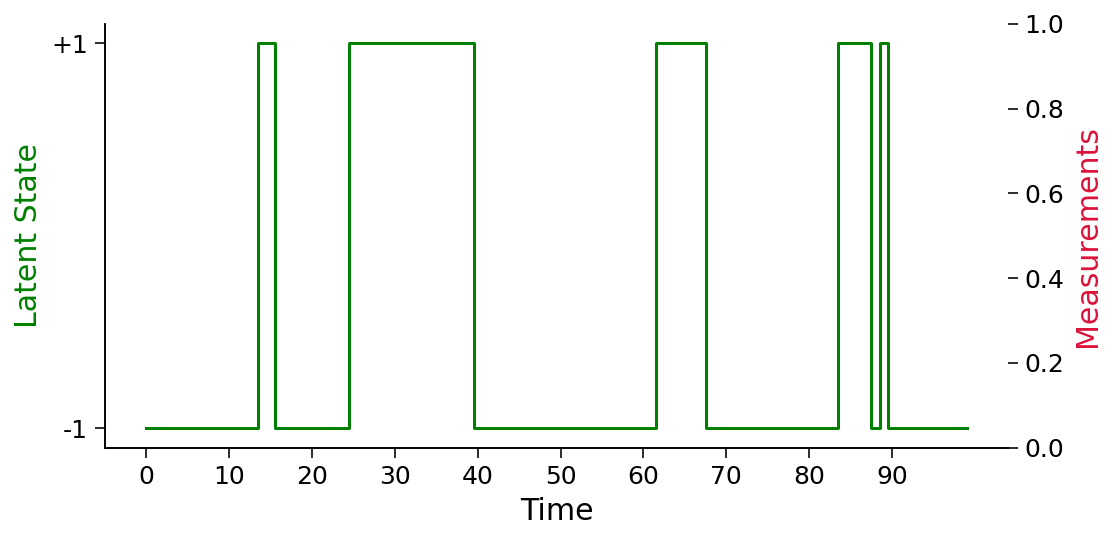
\includegraphics[scale=0.25]{Figures/HD/HD_Figure3.png}
\end{center}
\end{subbox}
\begin{subbox}{subbox}{Applications}
\scriptsize

Measurements could be:
\begin{itemize}
    \item 
 fish caught at different times as the school of fish moves from left to right
\item membrane voltage when an ion channel changes between open and closed
\item EEG frequency measurements as the brain moves between sleep stat
\end{itemize}

\end{subbox}
\begin{subbox}{subbox}{Forgetting in a changing world}
\scriptsize



Even if we know the world state for sure, the world changes. We become less and less certain as time goes by since our last measurement. We'll plot how a Hidden Markov Model gradually "forgets" the current state when predicting the future without measurements.
\begin{center}
    
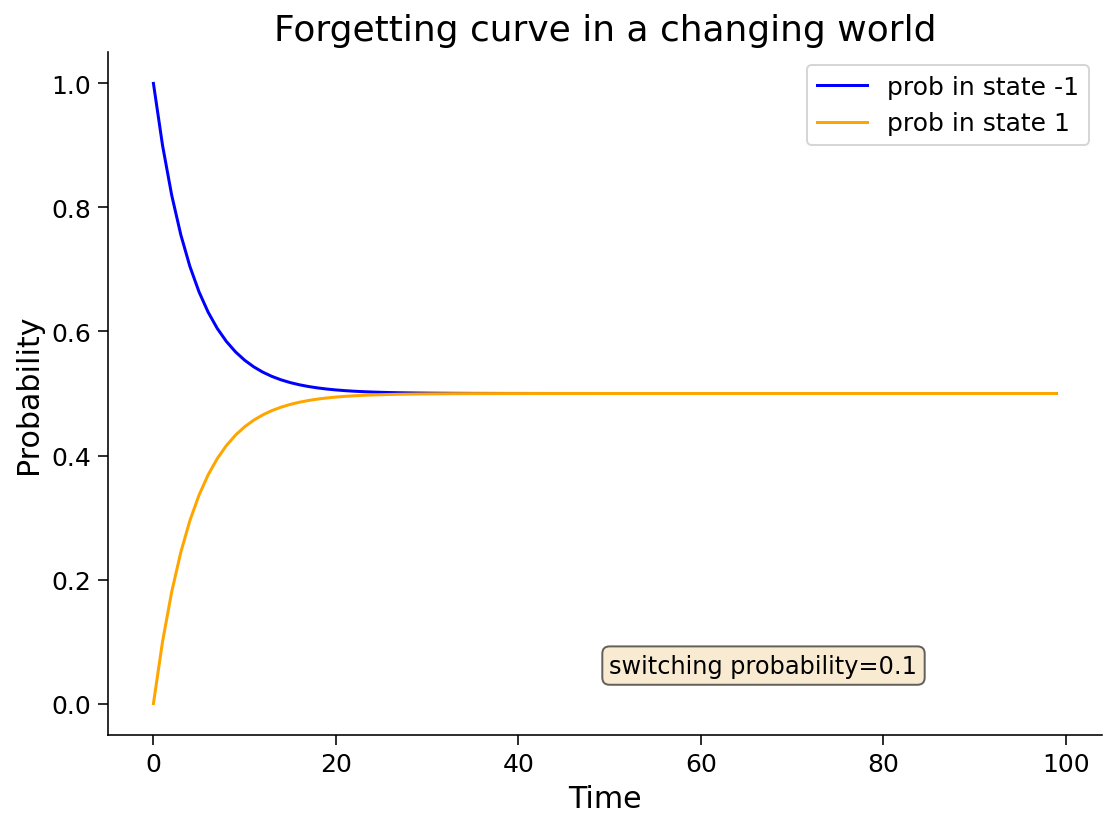
\includegraphics[scale=0.2]{Figures/HD/HD_Figure4.png}
\end{center}
\end{subbox}



\end{textbox}
%%%%%%%%%%%%%%%%%%%%%%%%% 
%%%%%%%%%%%%%%%%%%%%%%%%%
\begin{textbox}{\href{http://instructor.compneuro.neuromatch.io/tutorials/W3D2_HiddenDynamics/instructor/W3D2_Tutorial2.html}{Hidden Markov Model (W3D2T2)}   }

\begin{subbox}{subbox}{Forward inference of HMM}
\scriptsize
As a recursive algorithm, let's assume we already have yesterday's posterior from time $t-1$: $p(s_{t-1}|m_{1:t-1})$. When the new data $m_{t}$ comes in, the algorithm performs the following steps:\\

\textbf{Predict}: transform yesterday's posterior over $s_{t-1}$ into today's prior over $s_t$ using the transition matrix $D$:

\begin{equation*}
\text{today's prior}=p(s_t|m_{1:t-1})= p(s_{t-1}|m_{1:t-1}) D
\end{equation*}

\textbf{Update}: Incorporate measurement $m_t$ to calculate the posterior $p(s_t|m_{0:t})$

\begin{equation*}
\text{posterior} \propto \text{prior}\cdot \text{likelihood}=p(m_t|s_t)p(s_t|m_{0:t-1})
\end{equation*}


The plot below shows an example HMM simulation. 
\begin{center}
    
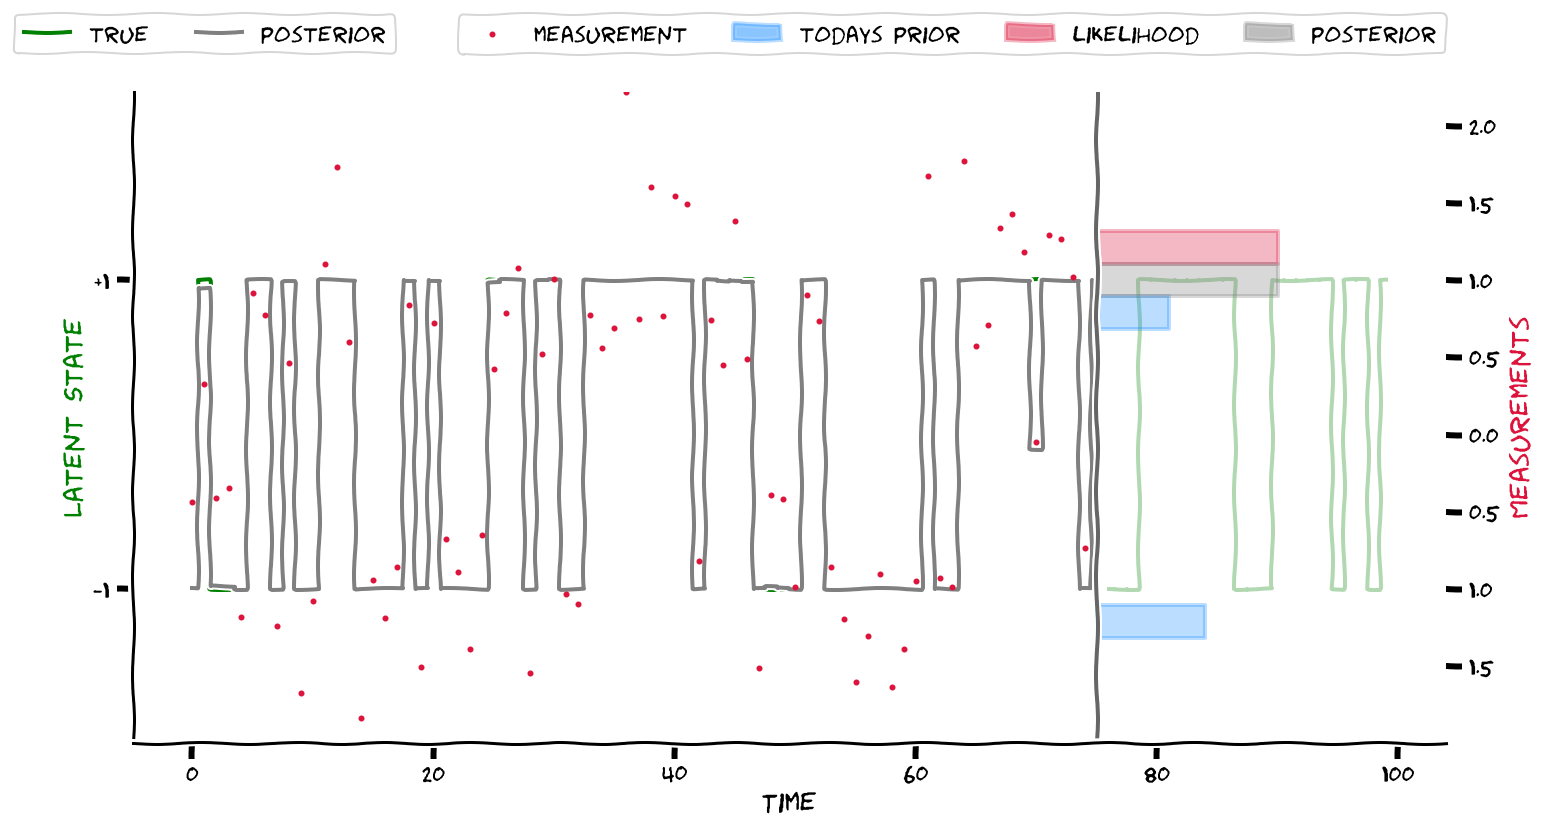
\includegraphics[scale=0.25]{Figures/HD/HD_Figure5.png}
\end{center}
\end{subbox}




\end{textbox}
%%%%%%%%%%%%%%%%%%%%%%%%% 
%%%%%%%%%%%%%%%%%%%%%%%%%
%%% TUTORIAL 3
\newpage
%%%%%%%%%%%%%%%%%%%%%%%%% 
%%%%%%%%%%%%%%%%%%%%%%%%%
\begin{textbox}{\href{http://instructor.compneuro.neuromatch.io/tutorials/W3D2_HiddenDynamics/instructor/W3D2_Tutorial3.html}{The Kalman Filter (W3D2T3)}   }

\begin{subbox}{subbox}{Application}
\scriptsize

We have used Hidden Markov Models (HMM) to infer \textit{discrete} latent states from a sequence of measurements. Here, we will learn how to infer a \textit{continuous} latent variable using the \textbf{Kalman filter}, which is one version of an HMM.

You can imagine this inference process happening as Mission Control tries to locate and track Astrocat. But you can also imagine that the brain is using an analogous Hidden Markov Model to track objects in the world, or to estimate the consequences of its own actions. And you could use this technique to estimate brain activity from noisy measurements, for understanding or for building a brain-machine interface.

\end{subbox}
\begin{subbox}{subbox}{Simulating Astrocat's movements}
\scriptsize
We will simulate how Astrocat moves based on stochastic linear dynamics.

The linear dynamical system 
$$ s_t = Ds_{t-1} + w_{t-1}$$
determines Astrocat's position $s_t$. $D$ is a scalar that models how Astrocat would like to change its position over time, and $w_t \sim \mathcal{N}(0, \sigma_p^2)$ is white Gaussian noise caused by unreliable actuators in Astrocat's propulsion unit. 

\begin{center}
    
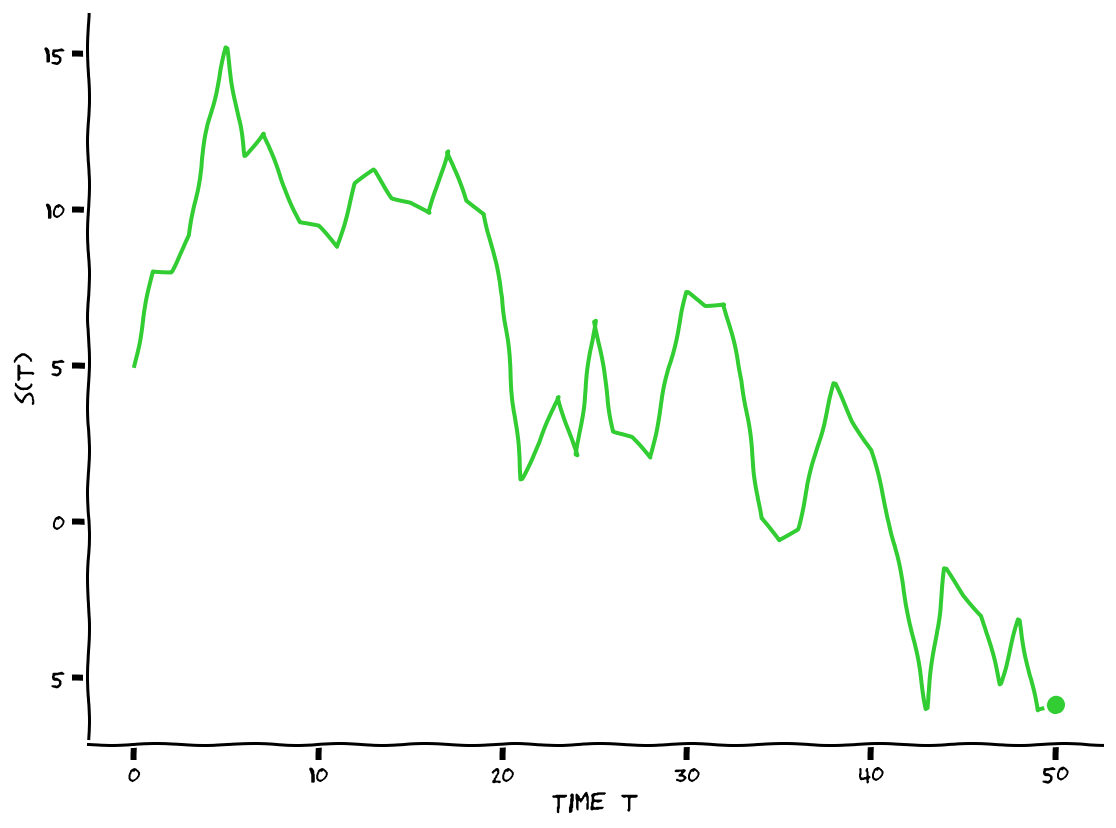
\includegraphics[scale=0.2]{Figures/HD/HD_Figure6.png}
\end{center}

\begin{enumerate}
    \item 
When D is large, the state at time step t will depend heavily on the state at time
   step $t_1$. If we forget about the noise term, D = 2 would mean that the state at each
   time step is double the one before! So the state becomes huge and basically explodes towards
   infinity.

\item If D is a large negative number, the state at time t will be a different sign than the
   state at time step $t_1$. So the state will oscillate over the x axis.

\item When D is zero, the state at time t will not depend on the previous state, it will just
   be drawn from the noise distribution.
   \end{enumerate} 
\end{subbox}

\end{textbox}
%%%%%%%%%%%%%%%%%%%%%%%%% 
%%%%%%%%%%%%%%%%%%%%%%%%%
\begin{textbox}{\href{http://instructor.compneuro.neuromatch.io/tutorials/W3D2_HiddenDynamics/instructor/W3D2_Tutorial3.html}{The Kalman Filter (W3D2T3)}   }

\begin{subbox}{subbox}{Implementing a Kalman filter}
\scriptsize

A Kalman filter estimates a posterior probability distribution \textit{recursively} over time using a mathematical model of the process and incoming measurements. This dynamic posterior allows us to improve our guess about Astrocat's position as new measures arrive; besides, its mean is the best estimate one can compute of Astrocat's actual position at each time step.

Follow this recipe to implement your own Kalman filter:

\textbf{Step 1: Change yesterday's posterior into today's prior}\\

Use the mathematical model to calculate how deterministic changes in the process shift yesterday's posterior, $\mathcal{N}(\mu_{s_{t-1}}, \sigma_{s_{t-1}}^2)$, and how random changes in the process broaden the shifted distribution:

\begin{align*}
p(s_t|m_{1:t-1}) &=& p(Ds_{t-1}+w_{t-1} | m_{1:t-1})\\ 
&=& \mathcal{N}(D\mu_{s_{t-1}} + 0, D^2\sigma_{s_{t-1}}^2 +\sigma_p^2)
\end{align*}

Note that we use $\sigma_p$ here to denote the process noise.

\textbf{Step 2: Multiply today's prior by likelihood} \\

Use the latest measurement of Astrocat's collar (fresh evidence) to form a new estimate somewhere between this measurement and what we predicted in Step 1. The next posterior is the result of multiplying the Gaussian computed in Step 1 (a.k.a. today's prior) and the likelihood, which is also modeled as a Gaussian $\mathcal{N}(m_t, \sigma_m^2)$:

\texbf{Step 2a: add information from prior and likelihood}\\

To find the posterior variance, we first compute the posterior information (which is the inverse of the variance) by adding the information provided by the prior and the likelihood:

\begin{equation}
\frac{1}{\sigma_{s_t}^2} = \frac{1}{D^2\sigma_{s_{t-1}}^2 +\sigma_p^2} + \frac{1}{\sigma_m^2}
\end{equation}

Now we can take the inverse of the posterior information to get back the posterior variance.

\textbf{Step 2b: add means from prior and likelihood}\\ 

To find the posterior mean, we calculate a weighted average of means from prior and likelihood, where each weight, $g$, is just the fraction of information that each Gaussian provides!

\begin{align}
g_{\rm{prior}} &= \frac{\rm{information}_{\textit{ }\rm{prior}}}{\rm{information}_{\textit{ }\rm{posterior}}} \\
g_{\rm{likelihood}} &= \frac{\rm{information}_{\textit{ }\rm{likelihood}}}{\rm{information}_{\textit{ }\rm{posterior}}} \\
\bar{\mu}_t &= g_{\rm{prior}} D\mu_{s_{t-1}} + g_{\rm{likelihood}} m_t
\end{align}
\end{subbox}

\end{textbox}
%%%%%%%%%%%%%%%%%%%%%%%%% 
%%%%%%%%%%%%%%%%%%%%%%%%%
\begin{textbox}{\href{http://instructor.compneuro.neuromatch.io/tutorials/W3D2_HiddenDynamics/instructor/W3D2_Tutorial3.html}{The Kalman Filter (W3D2T3)}   }

\begin{subbox}{subbox}{Relationship to classic description of Kalman filter}
\scriptsize

We're teaching this recipe because it is interpretable and connects to past lessons about the sum rule and product rule for Gaussians. But the classic description of the Kalman filter is a little different. The above weights, $g_{\rm{prior}}$ and $g_{\rm{likelihood}}$, add up to $1$ and can be written one in terms of the other; then, if we let $K = g_{\rm{likelihood}}$, the posterior mean can be expressed as:

\begin{equation}
\bar{\mu}_t = (1-K) D\bar{\mu}_{t-1} + K m_t = D\bar{\mu}_{t-1} + K (m_t - D\bar{\mu}_{t-1})
\end{equation}

In classic textbooks, you will often find this expression for the posterior mean; $K$ is known as the Kalman gain and its function is to choose a value partway between the current measurement $m_t$ and the prediction from Step 1.


\begin{center}
    
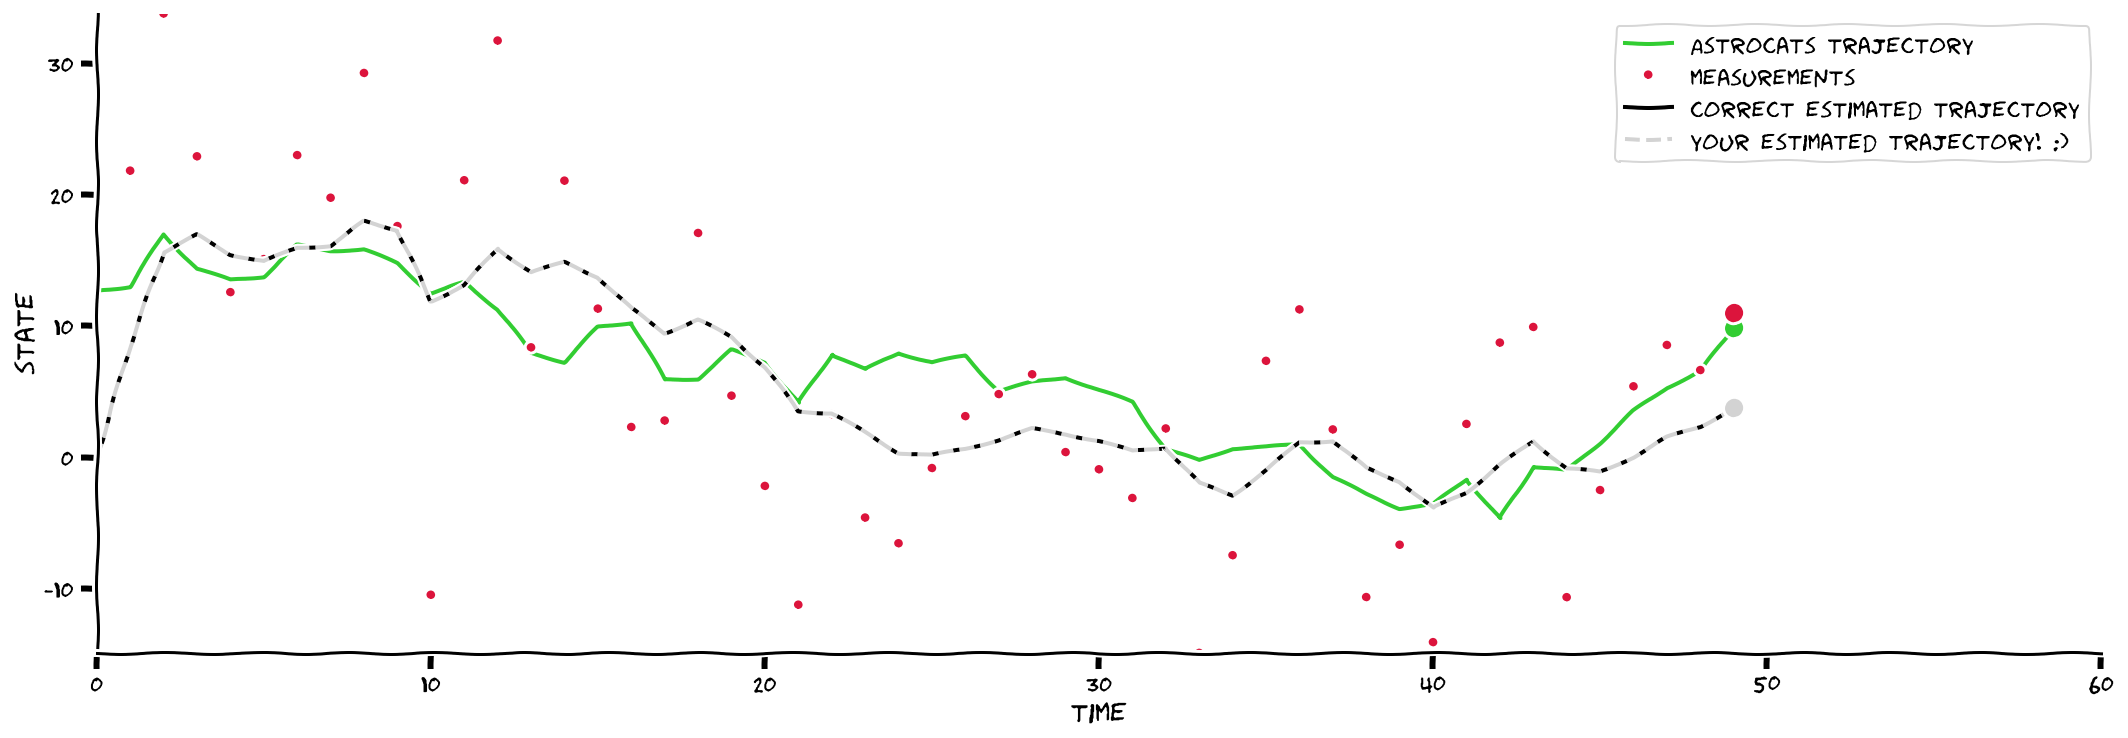
\includegraphics[scale=0.17]{Figures/HD/HD_Figure7.png}
\end{center}

\end{subbox}
\begin{subbox}{subbox}{Compare states, estimates, and measurements}
\scriptsize

How well do the estimates $\hat{s}$ match the actual values $s$? How does the distribution of errors $\hat{s}_t - s_t$ compare to the posterior variance? Why? Try different parameters of the Hidden Markov Model and observe how the properties change.

How do the measurements $m$ compare to the true states?


\begin{center}
    
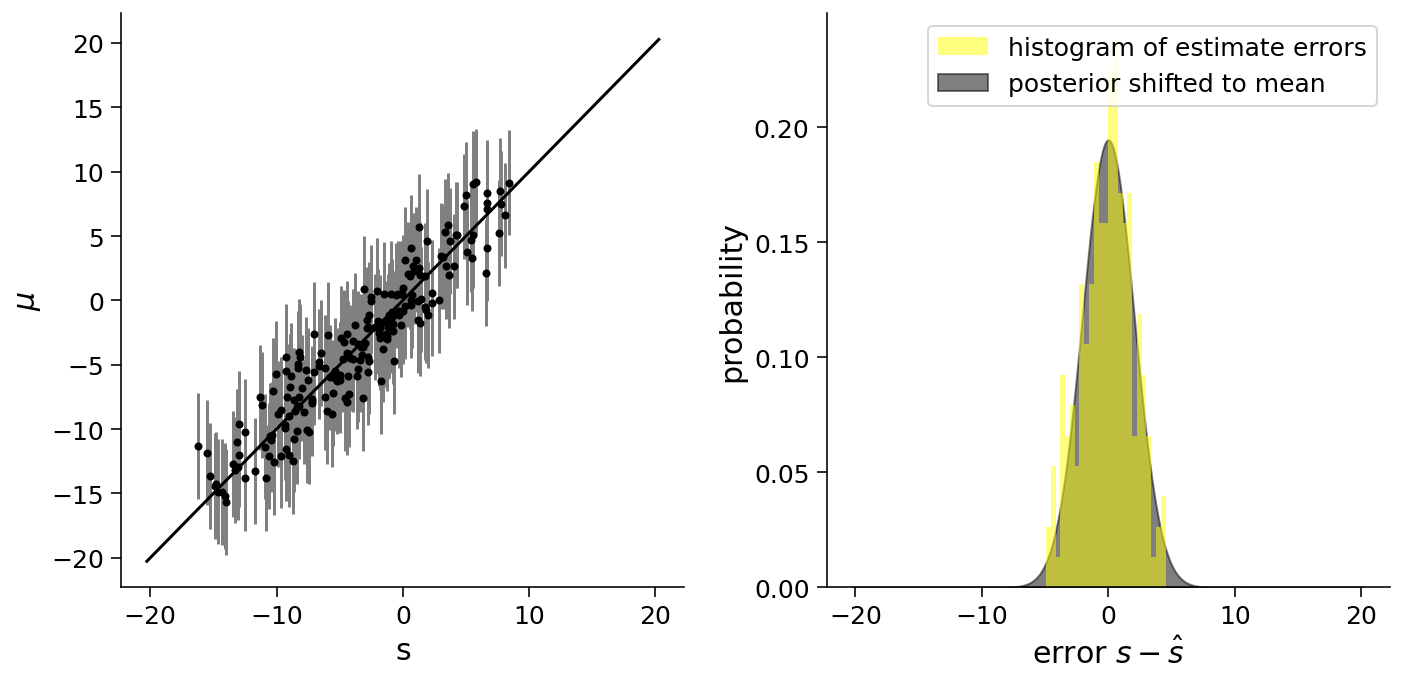
\includegraphics[scale=0.27]{Figures/HD/HD_Figure8.png}
\end{center}

\end{subbox}
\end{textbox}
%%%%%%%%%%%%%%%%%%%%%%%%% 
%%%%%%%%%%%%%%%%%%%%%%%%%
\begin{textbox}{\href{http://instructor.compneuro.neuromatch.io/tutorials/W3D2_HiddenDynamics/instructor/W3D2_Tutorial3.html}{The Kalman Filter (W3D2T3)}   }

\begin{subbox}{subbox}{ How long does it take to find astrocat?}
\scriptsize

Here we plot the posterior variance as a function of time. Before mission control gets measurements, their only information about astrocat's location is the prior. After some measurements, they hone in on astrocat.
\begin{itemize}
    \item 
 How does the variance shrink with time?
\item The speed depends on the process dynamics, but does it also depend on the signal-to-noise ratio (SNR)? (Here we measure SNR in decibels, a log scale where 1 dB means 0.1 log unit.)
\end{itemize}

The red curve shows how rapidly the latent variance equilibrates exponentially from an initial condition, with a time constant of $\sim 1/(1-D^2)$. 

\begin{center}
    
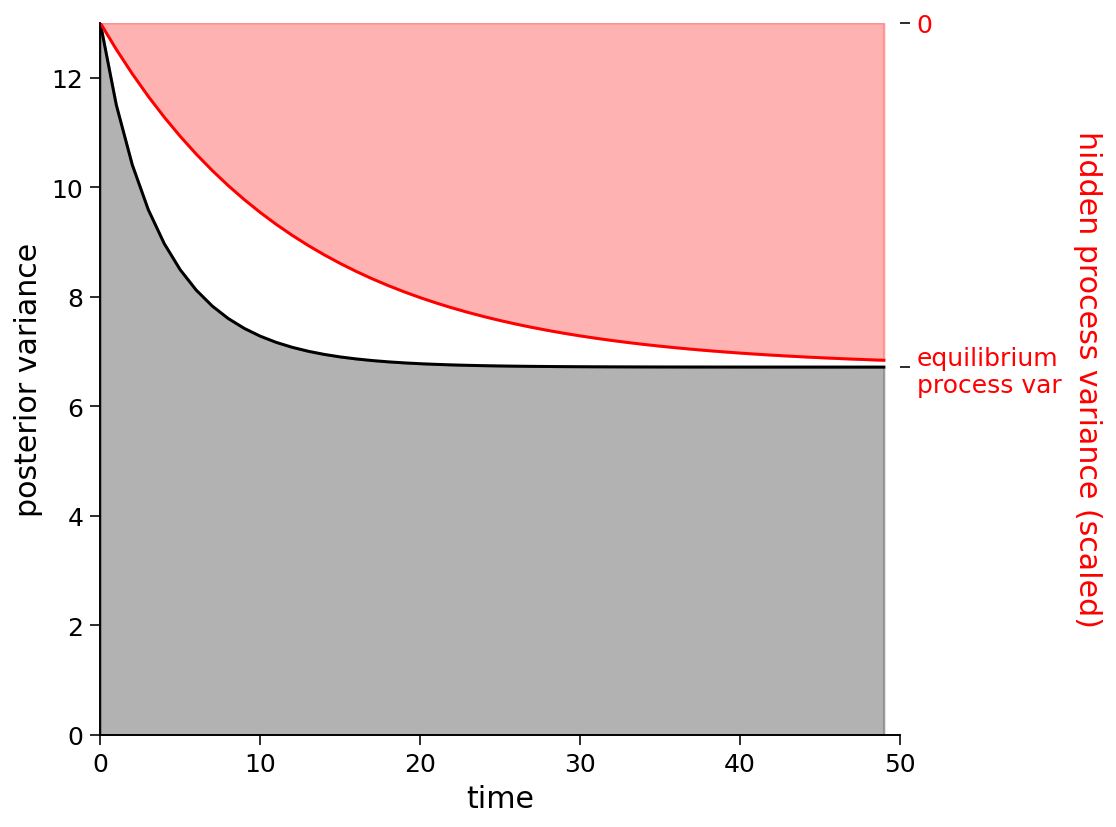
\includegraphics[scale=0.25]{Figures/HD/HD_Figure9.png}
\end{center}

\end{subbox}
\begin{subbox}{subbox}{ Applications of Kalman filter in brain science}
\scriptsize


\begin{itemize}
    \item  Brain-Computer Interface: estimate intended movements using neural activity as measurements.
\item Data analysis: estimate brain activity from noisy measurements (e.g., EEG)
\item Model of perception: prey tracking using noisy sensory measurements
\item Imagine your own! When are you trying to estimate something you cannot see directly?
\end{itemize}
There are many variants that improve upon the limitations of the Kalman filter: non-Gaussian states and measurements, nonlinear dynamics, and more.

\end{subbox}
\end{textbox}

\end{multicols}
\newpage
%%% Optimal Control 
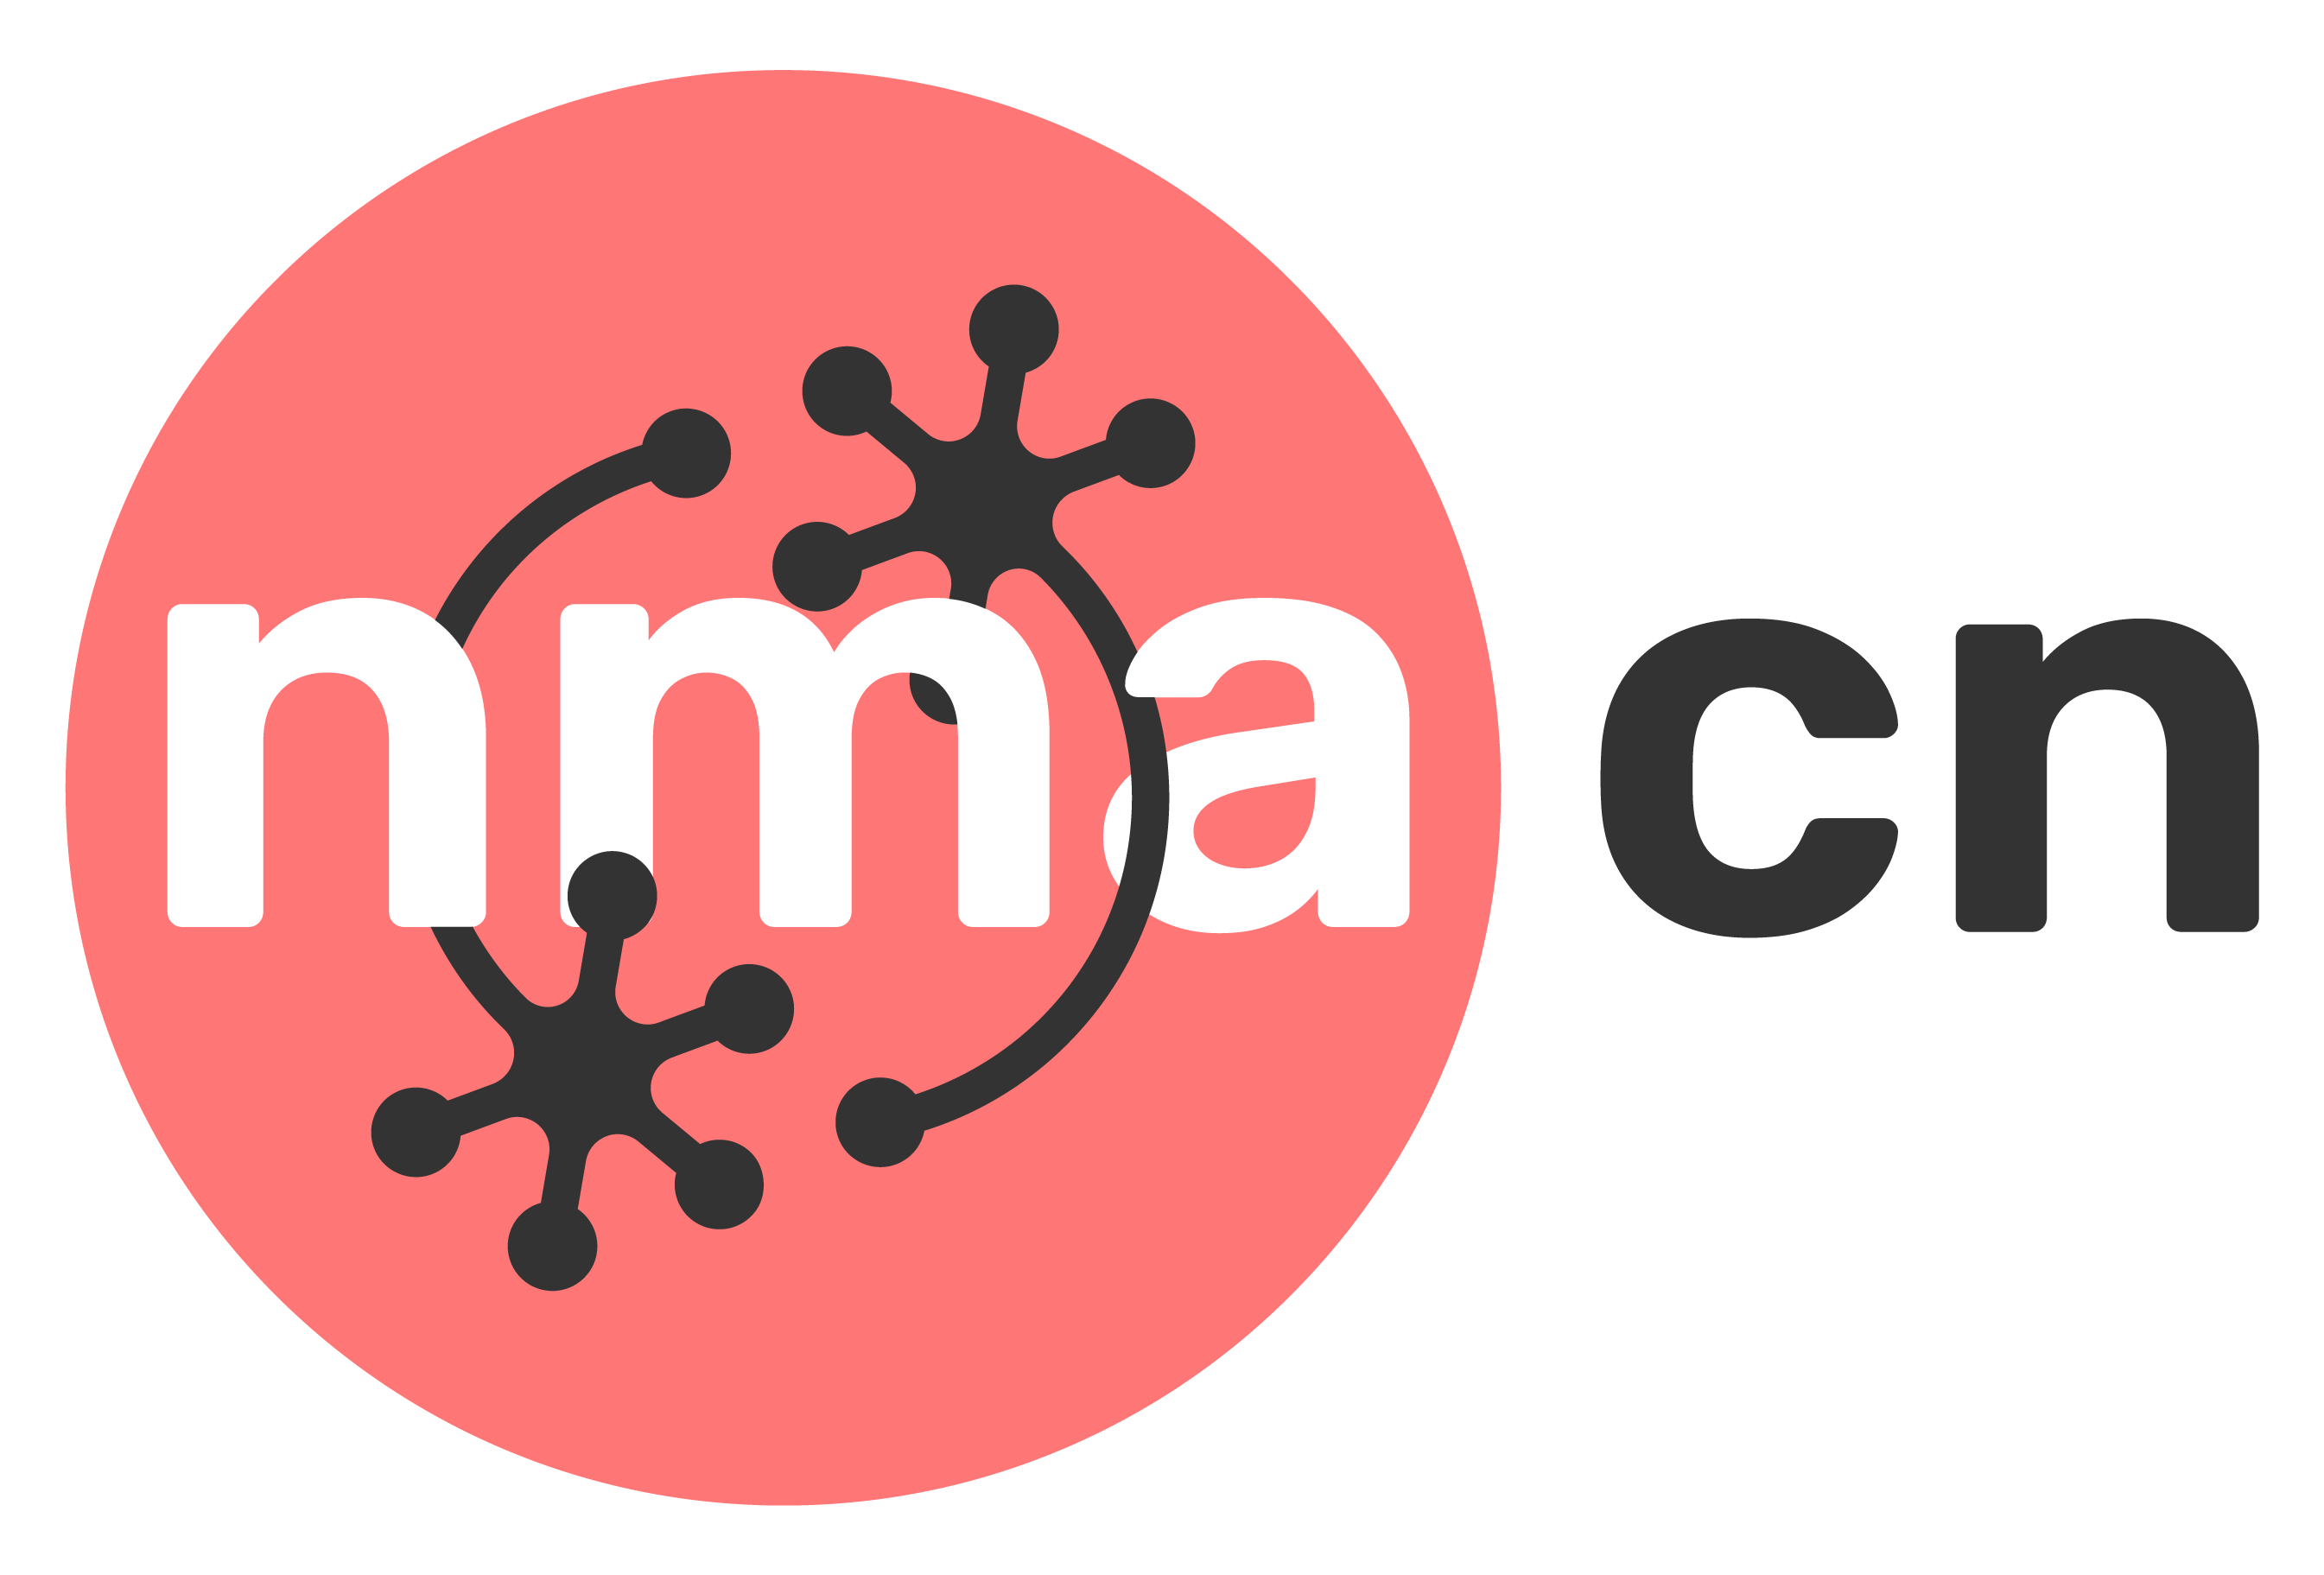
\includegraphics[scale=0.03]{Figures/NMACN.png}\href{https://compneuro.neuromatch.io/tutorials/intro.html}{\textbf{\Huge{Neuromatch Academy: Optimal Control - Summary Sheet}}\footnote{’t Hart et al., (2022). Neuromatch Academy: a 3-week, online summer school in computational neuroscience. Journal of Open Source Education, 5(49), 118. https://doi.org/10.21105/jose.00118}}
\small
\begin{multicols}{3}
\let\clearpage\relax
\begin{textbox}{\href{https://compneuro.neuromatch.io/tutorials/W3D3_OptimalControl/student/W3D3_Tutorial1.html}{Optimal Control for Discrete States }   }
\begin{subbox}{subbox}{Overview}
\scriptsize
Optimal Control combines ideas from the Hidden Dynamics lessons (which used Hidden Markov Models) with maximizing utility described in the Bayes day (which combined a posterior with a utility function). It also connects directly to later lessons in Reinforcement Learning, which learns how to control before you understand the world. In contrast, Optimal Control assumes that you already know how the world works.

Optimal Control is a crucial model in motor neuroscience, because it provides a principled benchmark for how we expect an animal should move. It also is an important engineering method, used for brain-computer interfaces and clamping neurons to desired activity patterns.

\end{subbox}

\begin{subbox}{subbox}{Objective}
\scriptsize
Here, we will implement a \textbf{binary control} task: a Partially Observable Markov Decision Process (POMDP) that describes fishing. The agent (you) seeks reward from two fishing sites without directly observing where the school of fish is (yes, a group of fish is called a school!). This makes the world a Hidden Markov Model (HMM). Based on when and where you catch fish, you keep updating your belief about the fish location, i.e., the posterior of the fish given past observations. You should control your position to get the most fish while minimizing the cost of switching sides.

You've already learned about stochastic dynamics, latent states, and measurements. These first exercises largely repeat your previous work. Now we introduce \textbf{actions}, based on the new concepts of \textbf{control, utility, and policy}. This general structure provides a foundational model for the brain's computations because it includes a perception-action loop where the animal can gather information, draw inferences about its environment, and select actions with the greatest benefit. \textit{How}, mechanistically, the neurons could actually implement these calculations is a separate question we don't address in this lesson.

We will:
\begin{itemize}
    \item 
 Use the Hidden Markov Models you learned about previously to model the world state.
    \item  Use the observations (fish caught) to build beliefs (posterior distributions) about the fish location.
    \item  Evaluate the quality of different control policies for choosing actions.
    \item  Discover the policy that maximizes utility.
\end{itemize}

\end{subbox}
\end{textbox}
%%%%%%%%%%%%%%%%%%%%%%%%% 
%%%%%%%%%%%%%%%%%%%%%%%%%
\begin{textbox}{\href{https://compneuro.neuromatch.io/tutorials/W3D3_OptimalControl/student/W3D3_Tutorial1.html}{Optimal Control for Discrete States }   }
\begin{subbox}{subbox}{Analyzing the Problem}
\scriptsize
\textbf{Problem Setting}\\

\textbf{1. State dynamics:} There are two possible locations for the fish: Left and Right. Secretly, at each time step, the fish may switch sides with a certain probability $p_{\rm sw} = 1 - p_{\rm stay}$. This is the binary switching model (\textit{Telegraph process}) that you've seen in Linear Systems . The fish location, $s^{\rm fish}$, is latent; you get measurements about it when you try to catch fish, like in Hidden Dynamics. This gives you a \textit{belief} or posterior probability of the current location given your history of measurements.\\

\textbf{2. Actions}: Unlike past days, you can now \textbf{act} on the process! You may stay on your current location (Left or Right), or switch to the other side.\\

\textbf{3. Rewards and Costs:} You get rewarded for each fish you catch (one fish is worth 1 "point"). If you're on the same side as the fish, you'll catch more, with probability $q_{\rm high}$ per discrete time step. Otherwise, you may still catch some fish with probability $q_{\rm low}$. \\

You pay a price of $C$ points for switching to the other side. So you better decide wisely!

\textbf{Maximizing Utility}\\

To decide "wisely" and maximize your total utility (total points), you will follow a \textbf{policy} that prescribes what to do in any situation. Here the situation is determined by your location and your \textbf{belief} $b_t$ (posterior) about the fish location (remember that the fish location is a latent variable). 

In optimal control theory, the belief is the posterior probability over the latent variable given all the past measurements. It can be shown that maximizing the expected utility with respect to this posterior is optimal.

In our problem, the belief can be represented by a single number because the fish are either on the left or the right side. So we write: 

\begin{equation}
b_t = p(s^{\rm fish}_t = {\rm Right}\  |\  m_{0:t}, a_{0:t-1})
\end{equation}

where $m_{0:t}$ are the measurements and $a_{0:t-1}$ are the actions (stay or switch).

Finally, we will parameterize the policy by a simple threshold on beliefs: when your belief that fish are on your current side falls below a threshold $\theta$, you switch to the other side.

Here, you will discover that if you pick the right threshold, this simple policy happens to be optimal!

\end{subbox}

\end{textbox}
%%%%%%%%%%%%%%%%%%%%%%%%% 
%%%%%%%%%%%%%%%%%%%%%%%%%
\begin{textbox}{\href{https://compneuro.neuromatch.io/tutorials/W3D3_OptimalControl/student/W3D3_Tutorial1.html}{Optimal Control for Discrete States }   }
\begin{subbox}{subbox}{Analyzing the Problem}
\scriptsize
\textbf{Problem Setting}\\

\textbf{1. State dynamics:} There are two possible locations for the fish: Left and Right. Secretly, at each time step, the fish may switch sides with a certain probability $p_{\rm sw} = 1 - p_{\rm stay}$. This is the binary switching model (\textit{Telegraph process}) that you've seen in Linear Systems . The fish location, $s^{\rm fish}$, is latent; you get measurements about it when you try to catch fish, like in Hidden Dynamics. This gives you a \textit{belief} or posterior probability of the current location given your history of measurements.\\

\textbf{2. Actions}: Unlike past days, you can now \textbf{act} on the process! You may stay on your current location (Left or Right), or switch to the other side.\\

\textbf{3. Rewards and Costs:} You get rewarded for each fish you catch (one fish is worth 1 "point"). If you're on the same side as the fish, you'll catch more, with probability $q_{\rm high}$ per discrete time step. Otherwise, you may still catch some fish with probability $q_{\rm low}$. \\

You pay a price of $C$ points for switching to the other side. So you better decide wisely!

\textbf{Maximizing Utility}\\

To decide "wisely" and maximize your total utility (total points), you will follow a \textbf{policy} that prescribes what to do in any situation. Here the situation is determined by your location and your \textbf{belief} $b_t$ (posterior) about the fish location (remember that the fish location is a latent variable). 

In optimal control theory, the belief is the posterior probability over the latent variable given all the past measurements. It can be shown that maximizing the expected utility with respect to this posterior is optimal.

In our problem, the belief can be represented by a single number because the fish are either on the left or the right side. So we write: 

\begin{equation}
b_t = p(s^{\rm fish}_t = {\rm Right}\  |\  m_{0:t}, a_{0:t-1})
\end{equation}

where $m_{0:t}$ are the measurements and $a_{0:t-1}$ are the actions (stay or switch).

Finally, we will parameterize the policy by a simple threshold on beliefs: when your belief that fish are on your current side falls below a threshold $\theta$, you switch to the other side.

Here, you will discover that if you pick the right threshold, this simple policy happens to be optimal!

\end{subbox}

\end{textbox}
%%%%%%%%%%%%%%%%%%%%%%%%% 
%%%%%%%%%%%%%%%%%%%%%%%%%
\end{multicols}
\newpage
%%% Reinforcement Learning
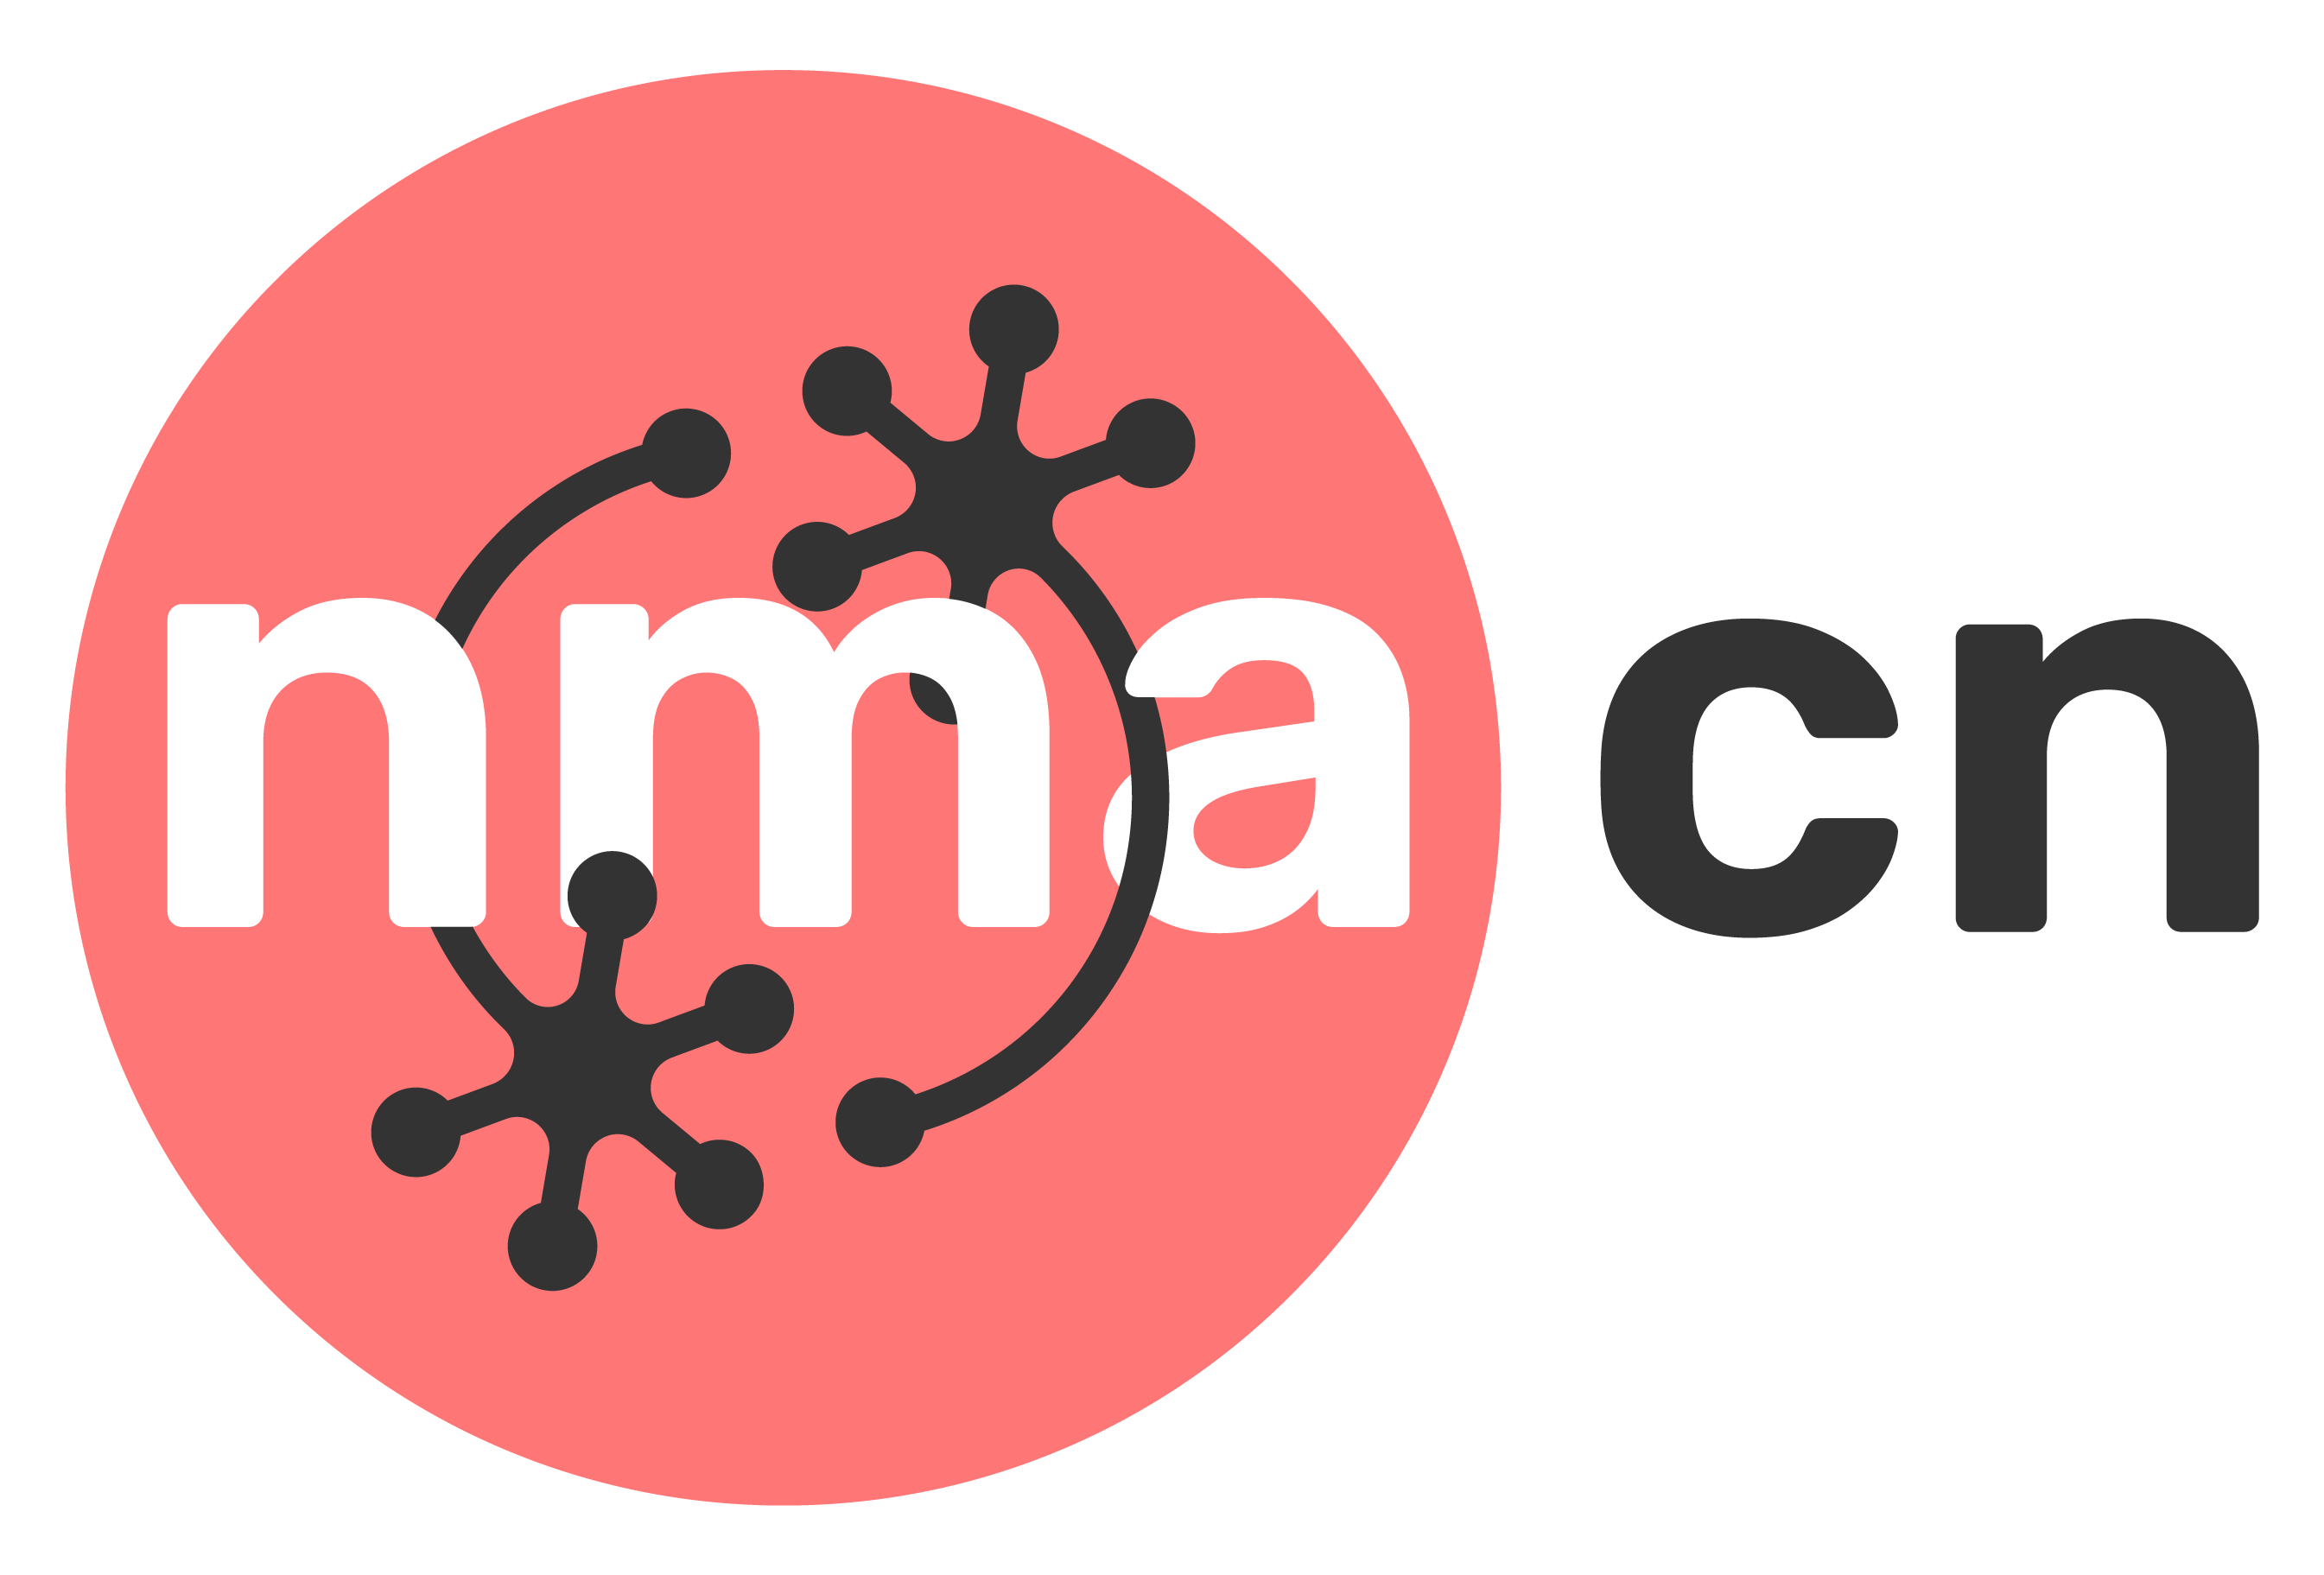
\includegraphics[scale=0.03]{Figures/NMACN.png}\href{https://compneuro.neuromatch.io/tutorials/intro.html}{\textbf{\Huge{Neuromatch Academy: Reinforcement Learning - Summary Sheet}}\footnote{’t Hart et al., (2022). Neuromatch Academy: a 3-week, online summer school in computational neuroscience. Journal of Open Source Education, 5(49), 118. https://doi.org/10.21105/jose.00118}}
%$\subsection*{Cheat Sheet}
\small

\begin{multicols}{3}

\let\clearpage\relax
\begin{textbox}{\href{https://compneuro.neuromatch.io/tutorials/W3D4_ReinforcementLearning/student/W3D4_Tutorial1.html}{Learning to Predict } }
\begin{subbox}{subbox}{Overview}
\scriptsize
Reinforcement Learning (RL) is a framework for defining and solving a learning problem where an animal or agent knows or infers the state of the world and then learns the value of the states and actions that can be taken in them, by receiving a reward signal. Importantly, reinforcement learning provides formal, optimal descriptions of learning first derived from studies of animal behavior and then validated when the formal quantities used in the model were observed in the brain in humans and animals. It is probably one of the most widely used computational approaches in neuroscience.


\end{subbox}
\begin{subbox}{subbox}{Learning to Predict}
\scriptsize
Here, we will learn how to estimate state-value functions in a classical conditioning paradigm using Temporal Difference (TD) learning and examine TD-errors at the presentation of the conditioned and unconditioned stimulus (CS and US) under different CS-US contingencies. This will provide you with an understanding of both how reward prediction errors (RPEs) behave in classical conditioning and what we should expect to see if Dopamine represents a "canonical" model-free RPE. 

\end{subbox}

\begin{subbox}{subbox}{Temporal difference learning}
\scriptsize
\textbf{Environment:}
\begin{itemize}

\item The agent experiences the environment in episodes or trials. 
\item Episodes terminate by transitioning to the inter-trial-interval (ITI) state and they are initiated from the ITI state as well. We clamp the value of the terminal/ITI states to zero. 
\item The classical conditioning environment is composed of a sequence of states that the agent deterministically transitions through. Starting at State 0, the agent moves to State 1 in the first step, from State 1 to State 2 in the second, and so on.  These states represent time in the tapped delay line representation
\item Within each episode, the agent is presented with a CS and US (reward). 
\item The CS is always presented at 1/4 of the total duration of the trial. The US (reward) is then delivered after the CS. The interval between the CS and US is specified by \textit{reward time}.
\item The agent's goal is to learn to predict expected rewards from each state in the trial. 
\end{itemize}

\end{subbox}


\end{textbox}
%%%%%%%%%%%%%%%%%%%%%%%%%%%%%%%%%%%%%%%%%%%%%%%%%%%%%%
%%%%%%%%%%%%%%%%%%%%%%%%%%%%%%%%%%%%%%%%%%%%%%%%%%%%%%
\begin{textbox}{\href{https://compneuro.neuromatch.io/tutorials/W3D4_ReinforcementLearning/student/W3D4_Tutorial1.html}{Learning to Predict } }
\begin{subbox}{subbox}{General concepts}
\scriptsize


Return $G_{t}$: future cumulative reward, which can be written in a recursive form
\begin{align}
G_{t} &= \sum \limits_{k = 0}^{\infty} \gamma^{k} r_{t+k+1} \\
&= r_{t+1} + \gamma G_{t+1}
\end{align}

where $\gamma$ is discount factor that controls the importance of future rewards, and $\gamma \in [0, 1]$. $\gamma$ may also be interpreted as probability of continuing the trajectory.

Value function $V_{\pi}(s_t=s)$: expectation of the return

\begin{align}
V_{\pi}(s_t=s) &= \mathbb{E} [ G_{t}\; | \; s_t=s, a_{t:\infty}\sim\pi] \\
& = \mathbb{E} [ r_{t+1} + \gamma G_{t+1}\; | \; s_t=s, a_{t:\infty}\sim\pi]
\end{align}

With an assumption of \textbf{Markov process}, we thus have:

\begin{align}
V_{\pi}(s_t=s) &= \mathbb{E} [ r_{t+1} + \gamma V_{\pi}(s_{t+1})\; | \; s_t=s, a_{t:\infty}\sim\pi] \\
&= \sum_a \pi(a|s) \sum_{r, s'}p(s', r)(r + V_{\pi}(s_{t+1}=s'))
\end{align}
\end{subbox}
\begin{subbox}{subbox}{Temporal difference (TD) learning}
\scriptsize

With a Markovian assumption, we can use $V(s_{t+1})$ as an imperfect proxy for the true value $G_{t+1}$ (Monte Carlo bootstrapping), and thus obtain the generalized equation to calculate TD-error:

\begin{equation}
\delta_{t} = r_{t+1} + \gamma V(s_{t+1}) - V(s_{t})
\end{equation}

Value updated by using the learning rate constant $\alpha$:
\begin{equation}
V(s_{t}) \leftarrow V(s_{t}) + \alpha \delta_{t}
\end{equation}

Reference: \href{https://web.stanford.edu/group/pdplab/pdphandbook/handbookch10.html}{Temporal-Difference Learning}


\end{subbox}
\begin{subbox}{subbox}{Definitions}
\scriptsize
TD-error:
\begin{equation}
\delta_{t} = r_{t+1} + \gamma V(s_{t+1}) - V(s_{t})
\end{equation}
Value updates:
\begin{equation}
V(s_{t}) \leftarrow V(s_{t}) + \alpha \delta_{t}
\end{equation}

\end{subbox}
\end{textbox}
%%%%%%%%%%%%%%%%%%%%%%%%%%%%%%%%%%%%%%%%%%%%%%%%%%%%%%
%%%%%%%%%%%%%%%%%%%%%%%%%%%%%%%%%%%%%%%%%%%%%%%%%%%%%%
\begin{textbox}{\href{https://compneuro.neuromatch.io/tutorials/W3D4_ReinforcementLearning/student/W3D4_Tutorial1.html}{Learning to Predict } }
\begin{subbox}{subbox}{TD-learning with guaranteed rewards}
\scriptsize

TD-learning to estimate the state-value function in the classical-conditioning world with guaranteed rewards, with a fixed magnitude, at a fixed delay after the conditioned stimulus, CS. Save TD-errors over learning (i.e., over trials) so we can visualize them afterwards. 

To simulate the effect of the CS, you should only update $V(s_{t})$ during the delay period after CS. This period is indicated by the boolean variable \textit{is delay}. This can be implemented by multiplying the expression for updating the value function by \textit{is delay}.

\begin{center}
    
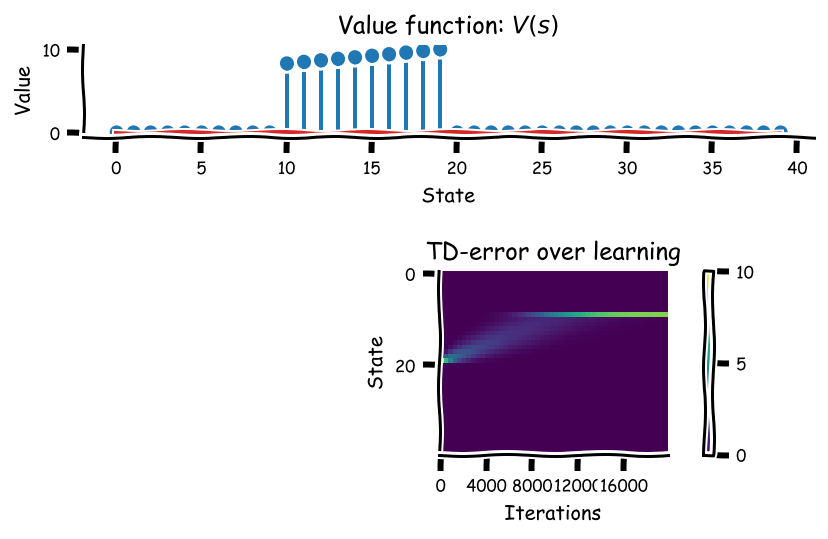
\includegraphics[scale=0.18]{Figures/RL/RL_Figure1.png}
\end{center}

\end{subbox}
\begin{subbox}{subbox}{US to CS Transfer }
\scriptsize

During classical conditioning, the subject's behavioral response (e.g., salivating) transfers from the unconditioned stimulus (US; like the smell of tasty food) to the conditioned stimulus (CS; like Pavlov ringing his bell) that predicts it. Reward prediction errors play an important role in this process by adjusting the value of states according to their expected, discounted return.

Use the widget below to examine how reward prediction errors change over time. 


Before training (orange line), only the reward state has high reward prediction error. As training progresses (blue line, slider), the reward prediction errors shift to the conditioned stimulus, where they end up when the trial is complete (green line). 

Dopamine neurons, which are thought to carry reward prediction errors \textit{in vivo}, show exactly the same behavior!
\begin{center}
    
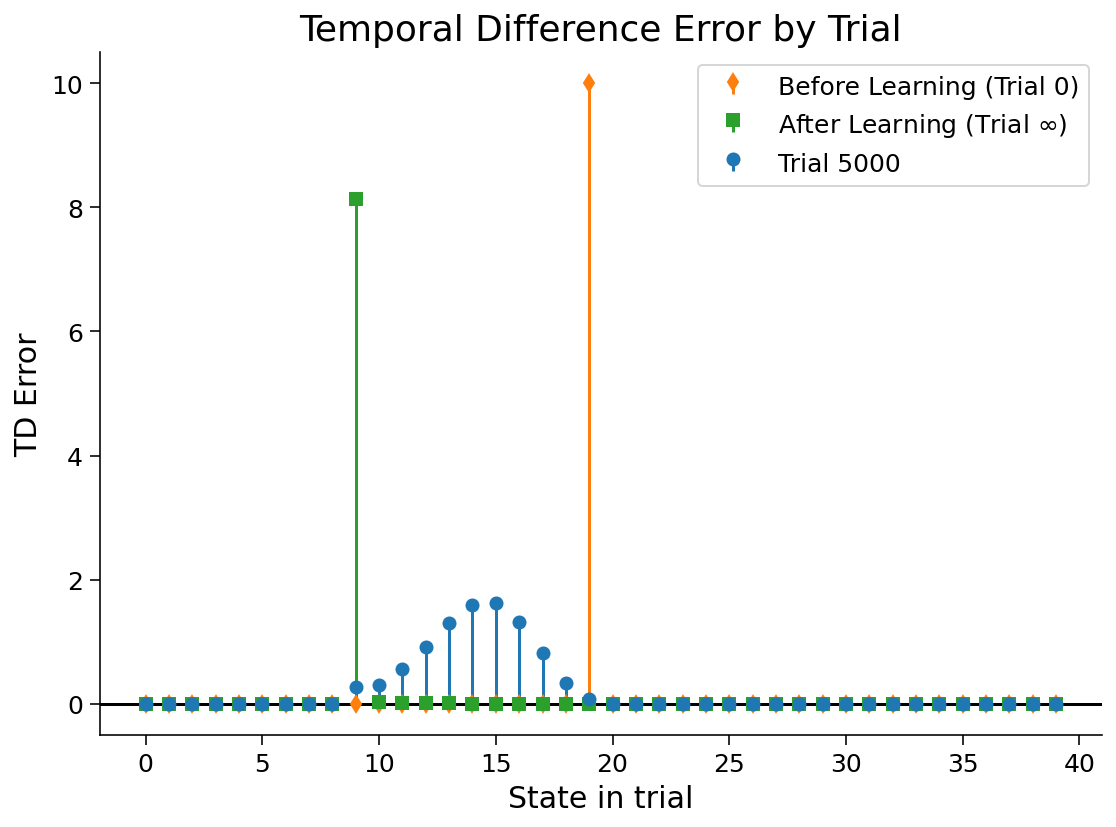
\includegraphics[scale=0.15]{Figures/RL/RL_Figure2.png}
\end{center}

\end{subbox}
\end{textbox}
%%%%%%%%%%%%%%%%%%%%%%%%%%%%%%%%%%%%%%%%%%%%%%%%%%%%%%
%%%%%%%%%%%%%%%%%%%%%%%%%%%%%%%%%%%%%%%%%%%%%%%%%%%%%%
\begin{textbox}{\href{https://compneuro.neuromatch.io/tutorials/W3D4_ReinforcementLearning/student/W3D4_Tutorial1.html}{Learning to Predict } }
\begin{subbox}{subbox}{Learning Rates and Discount Factors}
\scriptsize


Our TD-learning agent has two parameters that control how it learns: $\alpha$, the learning rate, and $\gamma$, the discount factor. In Exercise 1, we set these parameters to $\alpha=0.001$ and $\gamma=0.98$ for you. Here, you'll investigate how changing these parameters alters the model that TD-learning learns.

Before enabling the interactive demo below, take a moment to think about the functions of these two parameters. $\alpha$ controls the size of the Value function updates produced by each TD-error. In our simple, deterministic world, will this affect the final model we learn? Is a larger $\alpha$ necessarily better in more complex, realistic environments?

The discount rate $\gamma$ applies an exponentially-decaying weight to returns occuring in the future, rather than the present timestep. How does this affect the model we learn? What happens when $\gamma=0$ or $\gamma \geq 1$?

Use the widget to test your hypotheses.

\begin{center}
    
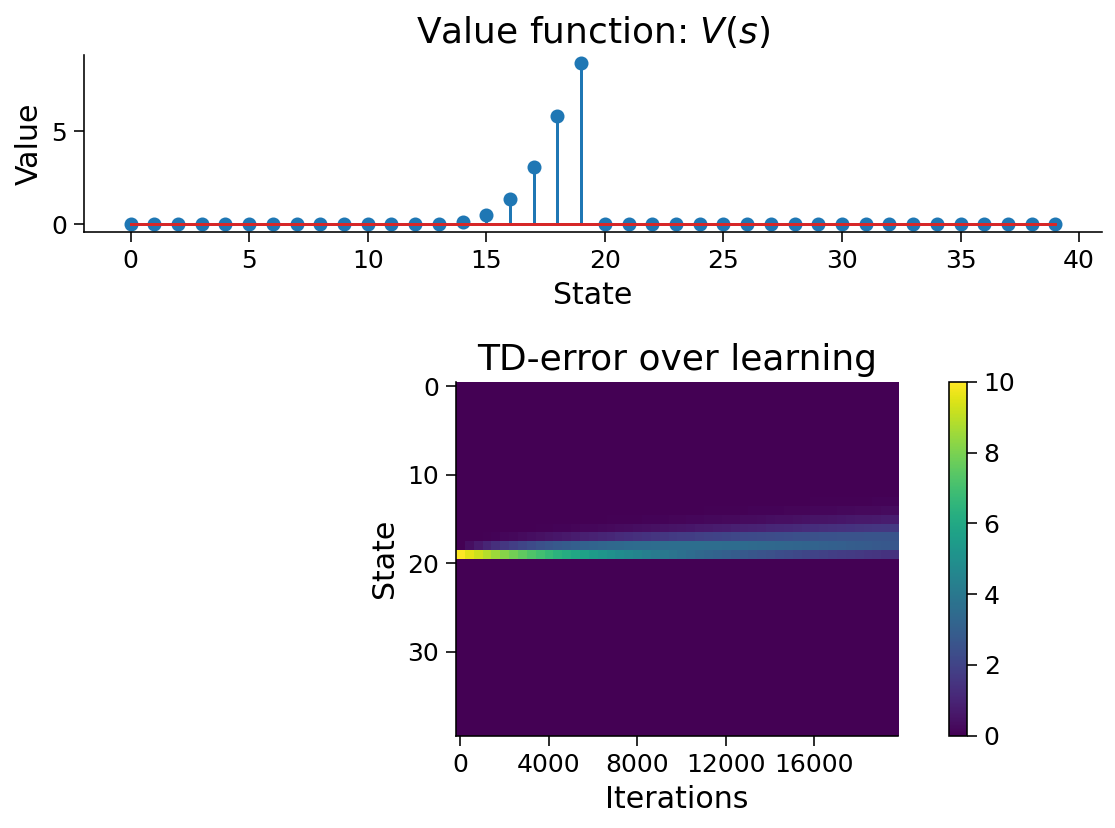
\includegraphics[scale=0.3]{Figures/RL/RL_Figure3.png}
\end{center}
$\alpha$ determines how fast the model learns. In the simple, deterministic world
we're using here, this allows the model to quickly converge onto the "true"
model that heavily values the conditioned stimulus. In more complex environments,
however, excessively large values of alpha can slow, or even prevent, learning,
as we'll see later.
$\gamma$ effectively controls how much the model cares about the future: larger values of
$\gamma$ cause the model to weigh future rewards nearly as much as present ones. At $\gamma$=1,
the model weights all rewards, regardless of when they occur, equally and when greater than one, it
starts to prefer rewards in the future, rather than the present (this is rarely good).
When $\gamma$=0, however, the model becomes greedy and only considers rewards that
can be obtained immediately.

\end{subbox}



\end{textbox}
%%%%%%%%%%%%%%%%%%%%%%%%%%%%%%%%%%%%%%%%%%%%%%%%%%%%%%
%%%%%%%%%%%%%%%%%%%%%%%%%%%%%%%%%%%%%%%%%%%%%%%%%%%%%%
\begin{textbox}{\href{https://compneuro.neuromatch.io/tutorials/W3D4_ReinforcementLearning/student/W3D4_Tutorial1.html}{Learning to Predict } }
\begin{subbox}{subbox}{TD-learning with varying reward magnitudes}
\scriptsize
In the previous exercise, the environment was as simple as possible. On every trial, the CS predicted the same reward, at the same time, with 100\% certainty. In the next few exercises, we will make the environment more progressively more complicated and examine the TD-learner's behavior.
\begin{center}
    
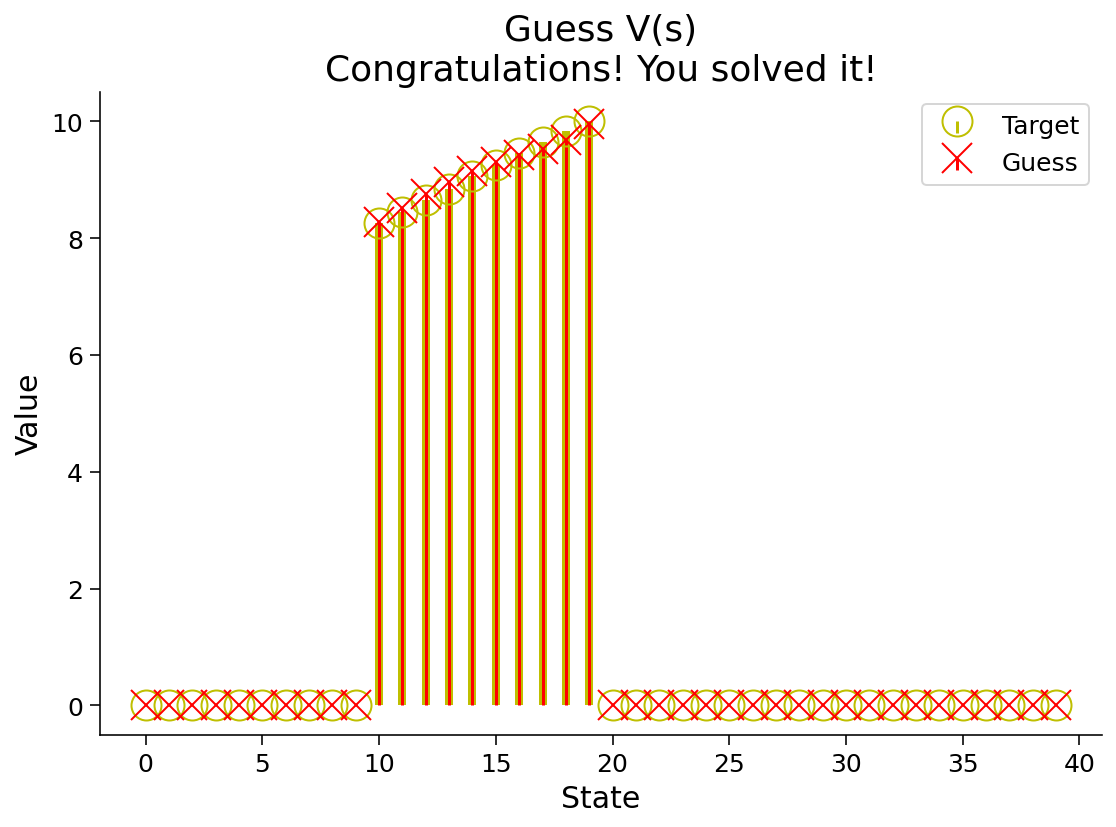
\includegraphics[scale=0.15]{Figures/RL/RL_Figure4.png}
\end{center}

\end{subbox}
\begin{subbox}{subbox}{Examining the TD Error}
\scriptsize
The plot below shows the TD errors from our multi-reward environment. A new feature appears in this plot? What is it? Why does it happen?
\begin{center}
    
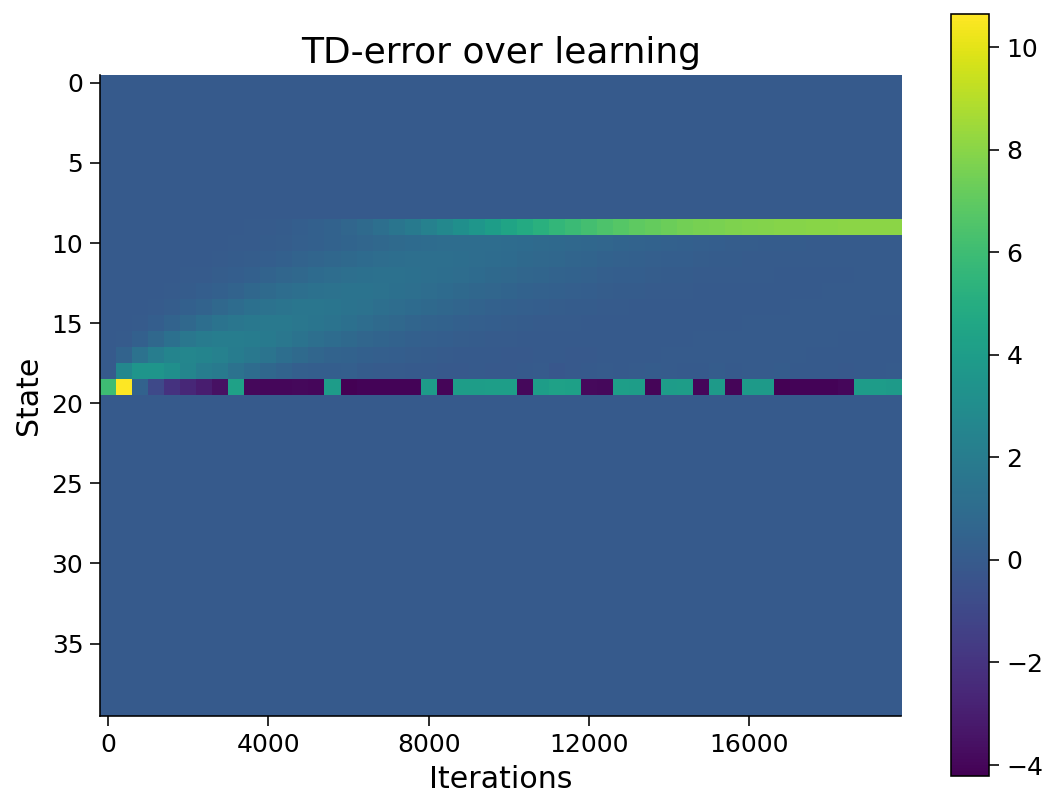
\includegraphics[scale=0.15]{Figures/RL/RL_Figure5.png}
\end{center}

\end{subbox}


\begin{subbox}{subbox}{TD-learning with probabilistic rewards}
\scriptsize
In this environment, we'll return to delivering a single reward of ten units. However, it will be delivered intermittently: on 20 percent of trials, the CS will be shown but the agent will not receive the usual reward; the remaining 80\% will proceed as usual.

 Run the cell below to simulate. How does this compare with the previous experiment?

Earlier in the notebook, we saw that changing $\alpha$ had little effect on learning in a deterministic environment. What happens if you set it to a large value, like 1, in this noisier scenario? Does it seem like it will \textit{ever} converge?
\begin{center}
    
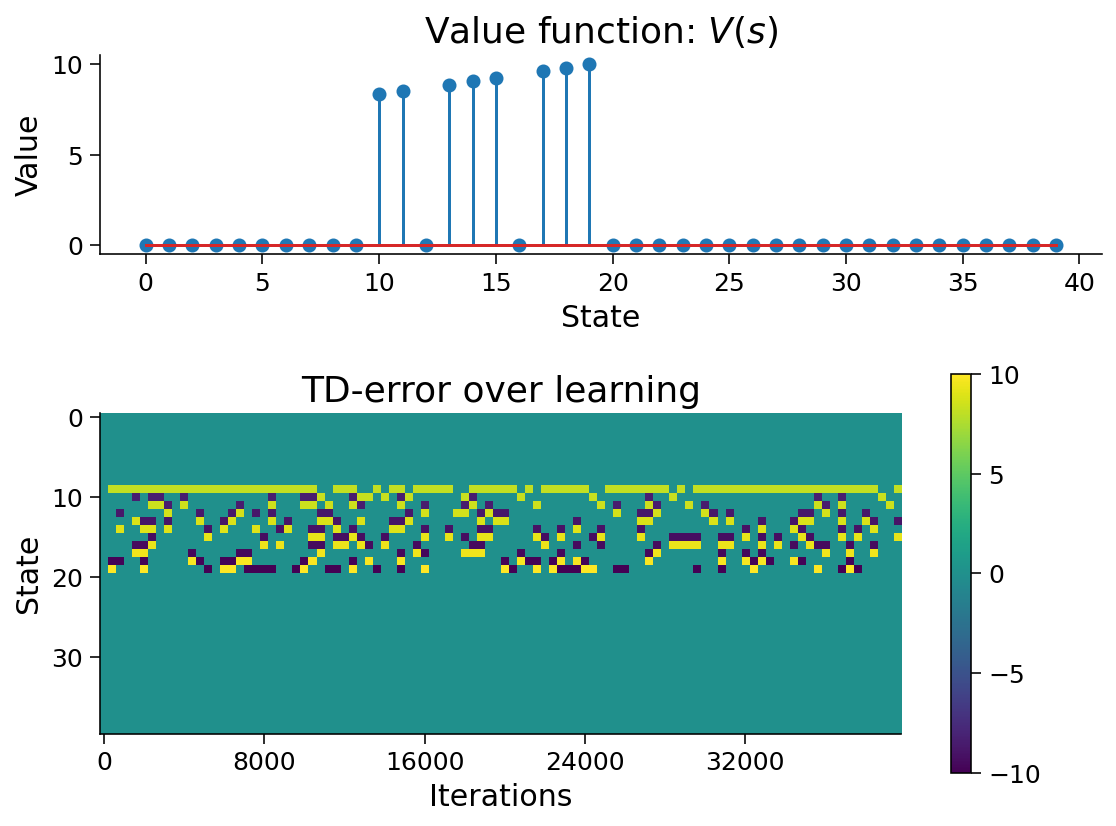
\includegraphics[scale=0.2]{Figures/RL/RL_Figure6.png}
\end{center}

\end{subbox}
\end{textbox}
%%%%%%%%%%%%%%%%%%%%%%%%%%%%%%%%%%%%%%%%%%%%%%%%%%%%%%
%%%%%%%%%%%%%%%%%%%%%%%%%%%%%%%%%%%%%%%%%%%%%%%%%%%%%%
\begin{textbox}{\href{https://compneuro.neuromatch.io/tutorials/W3D4_ReinforcementLearning/student/W3D4_Tutorial1.html}{Learning to Predict } }
\begin{subbox}{subbox}{Summary}
\scriptsize
Here, we have developed a simple TD Learner and examined how its state representations and reward prediction errors evolve during training. By manipulating its environment and parameters ($\alpha$, $\gamma$), you developed an intuition for how it behaves. 

This simple model closely resembles the behavior of subjects undergoing classical conditioning tasks and the dopamine neurons that may underlie that behavior. You may have implemented TD-reset or used the model to recreate a common experimental error. The update rule used here has been extensively studied for \href{https://www.pnas.org/content/108/Supplement_3/15647}{more than 70 years} as a possible explanation for artificial and biological learning. 

However, you may have noticed that something is missing. We carefully calculated the value of each state, but did not use it to actually do anything. Using values to plan \textbf{Actions} is coming up next!

\end{subbox}
\end{textbox}
\newpage
%%%%%%%%%%%%%%%%%%%%%%%%%%%%%%%%%%%%%%%%%%%%%%%%%%%%%%
%%%%%%%%%%%%%%%%%%%%%%%%%%%%%%%%%%%%%%%%%%%%%%%%%%%%%%
%%%%%%%% TUTORIAL 2
%%%%%%%%%%%%%%%%%%%%%%%%%%%%%%%%%%%%%%%%%%%%%%%%%%%%%%
%%%%%%%%%%%%%%%%%%%%%%%%%%%%%%%%%%%%%%%%%%%%%%%%%%%%%%
\begin{textbox}{\href{https://compneuro.neuromatch.io/tutorials/W3D4_ReinforcementLearning/student/W3D4_Tutorial2.html}{Learning to Act: Multi-Armed Bandits } }
\begin{subbox}{subbox}{Multi-Armed Bandits}
\scriptsize
Consider the following learning problem. You are faced repeatedly with a choice among $k$ different options, or actions. After each choice you receive a reward signal in the form of a numerical value, where the larger value is the better. Your objective is to maximize the expected total reward over some time period, for example, over 1000 action selections, or time steps.

This is the original form of the k-armed bandit problem. This name derives from the colloquial name for a slot machine, the "one-armed bandit", because it has the one lever to pull, and it is often rigged to take more money than it pays out over time. The multi-armed bandit extension is to imagine, for instance, that you are faced with multiple slot machines that you can play, but only one at a time. Which machine should you play, i.e., which arm should you pull, which action should you take, at any given time to maximize your total payout.


\begin{center}
    
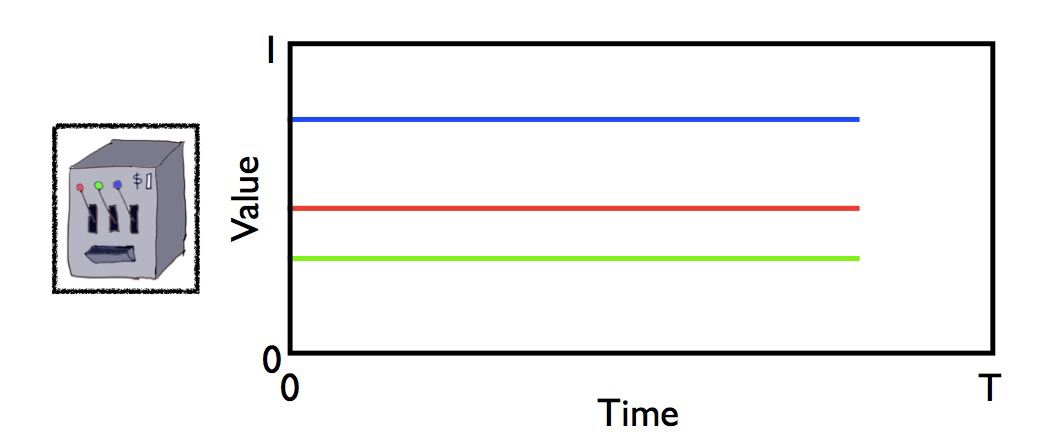
\includegraphics[scale=0.18]{Figures/RL/RL_Figure7.png}
\end{center}
While there are many different levels of sophistication and assumptions in how the rewards are determined, for simplicity's sake we will assume that each action results in a reward drawn from a fixed Gaussian distribution with unknown mean and unit variance. This problem setting is referred to as the \textit{environment}, and the goal is to find the arm with the highest mean value.

We will solve this \textit{optimization problem} with an \textit{agent}, in this case an algorithm that takes in rewards and returns actions.

\end{subbox}
\end{textbox}
%%%%%%%%%%%%%%%%%%%%%%%%%%%%%%%%%%%%%%%%%%%%%%%%%%%%%%
%%%%%%%%%%%%%%%%%%%%%%%%%%%%%%%%%%%%%%%%%%%%%%%%%%%%%%
\begin{textbox}{\href{https://compneuro.neuromatch.io/tutorials/W3D4_ReinforcementLearning/student/W3D4_Tutorial2.html}{Learning to Act: Multi-Armed Bandits } }
\begin{subbox}{subbox}{ Choosing an Action}
\scriptsize
The first thing our agent needs to be able to do is choose which arm to pull. The strategy for choosing actions based on our expectations is called a *policy* (often denoted $\pi$). We could have a random policy -- just pick an arm at random each time -- though this doesn't seem likely to be capable of optimizing our reward. We want some intentionality, and to do that we need a way of describing our beliefs about the arms' reward potential. We do this with an action-value function

\begin{equation}
q(a) = \mathbb{E} [r_{t} | a_{t} = a]
\end{equation}

where the value $q$ for taking action $a \in A$ at time $t$ is equal to the expected value of the reward $r_t$ given that we took action $a$ at that time. In practice, this is often represented as an array of values, where each action's value is a different element in the array.

Great, now that we have a way to describe our beliefs about the values each action should return, let's come up with a policy.

An obvious choice would be to take the action with the highest expected value. This is referred to as the \textit{greedy} policy

\begin{equation}
a_{t} = \text{argmax}_{a} \; q_{t} (a)
\end{equation}

where our choice action is the one that maximizes the current value function.

So far so good, but it can't be this easy. And, in fact, the greedy policy does have a fatal flaw: it easily gets trapped in local maxima. It never explores to see what it hasn't seen before if one option is already better than the others. This leads us to a fundamental challenge in coming up with effective policies.

\end{subbox}

\end{textbox}
%%%%%%%%%%%%%%%%%%%%%%%%%%%%%%%%%%%%%%%%%%%%%%%%%%%%%%
%%%%%%%%%%%%%%%%%%%%%%%%%%%%%%%%%%%%%%%%%%%%%%%%%%%%%%
\begin{textbox}{\href{https://compneuro.neuromatch.io/tutorials/W3D4_ReinforcementLearning/student/W3D4_Tutorial2.html}{Learning to Act: Multi-Armed Bandits } }

\begin{subbox}{subbox}{The Exploitation-Exploration Dilemma}
\scriptsize
If we never try anything new, if we always stick to the safe bet, we don't know what we are missing. Sometimes we aren't missing much of anything, and regret not sticking with our preferred choice, yet other times we stumble upon something new that was way better than we thought.

This is the exploitation-exploration dilemma: do you go with your best choice now, or risk the less certain option with the hope of finding something better. Too much exploration, however, means you may end up with a sub-optimal reward once it's time to stop.

In order to avoid getting stuck in local minima while also maximizing reward, effective policies need some way to balance between these two aims.

A simple extension to our greedy policy is to add some randomness. For instance, a coin flip -- heads we take the best choice now, tails we pick one at random. This is referred to as the $\epsilon$-greedy policy:

\begin{equation}
P (a_{t} = a) = 
        \begin{cases}
        1 - \epsilon + \epsilon/N    & \quad \text{if } a_{t} = \text{argmax}_{a} \; q_{t} (a) \\
        \epsilon/N        & \quad \text{else} 
        \end{cases} 
\end{equation}

which is to say that with probability 1 - $\epsilon$ for $\epsilon \in [0,1]$ we select the greedy choice, and otherwise we select an action at random (including the greedy option).

Despite its relative simplicity, the epsilon-greedy policy is quite effective, which leads to its general popularity.

The plot below shows the epsilon-greedy algorithm for deciding which action to take from a set of possible actions given their value function and a probability $\epsilon$ of simply choosing one at random. 
\begin{center}
    
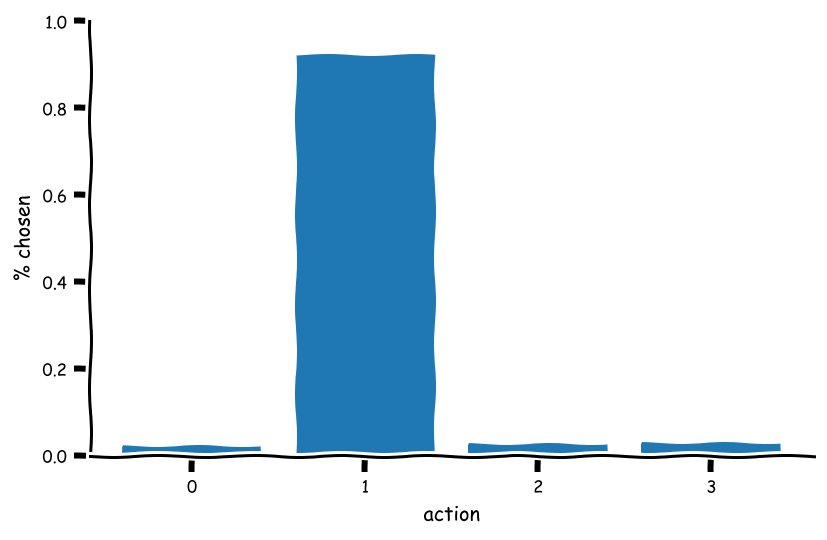
\includegraphics[scale=0.18]{Figures/RL/RL_Figure8.png}
\end{center}
This is what we should expect, that the action with the largest value (action 1) is selected about (1-$\epsilon$) of the time, or 90\% for $\epsilon = 0.1$, and the remaining 10\% is split evenly amongst the other options. Use the demo below to explore how changing $\epsilon$ affects the distribution of selected actions.

\end{subbox}
\end{textbox}
%%%%%%%%%%%%%%%%%%%%%%%%%%%%%%%%%%%%%%%%%%%%%%%%%%%%%%
%%%%%%%%%%%%%%%%%%%%%%%%%%%%%%%%%%%%%%%%%%%%%%%%%%%%%%
\begin{textbox}{\href{https://compneuro.neuromatch.io/tutorials/W3D4_ReinforcementLearning/student/W3D4_Tutorial2.html}{Learning to Act: Multi-Armed Bandits } }

\begin{subbox}{subbox}{Solving Multi-Armed Bandits}
\scriptsize

Now that we have both a policy and a learning rule, we can combine these to solve our original multi-armed bandit task. Recall that we have some number of arms that give rewards drawn from Gaussian distributions with unknown mean and unit variance, and our goal is to find the arm with the highest mean.

We can use our multi-armed bandit method to evaluate how our epsilon-greedy policy and learning rule perform at solving the task. First we will set our environment to have 10 arms and our agent parameters to $\epsilon=0.1$ and $\alpha=0.01$. In order to get a good sense of the agent's performance, we will run the episode for 1000 steps.
\begin{center}
    
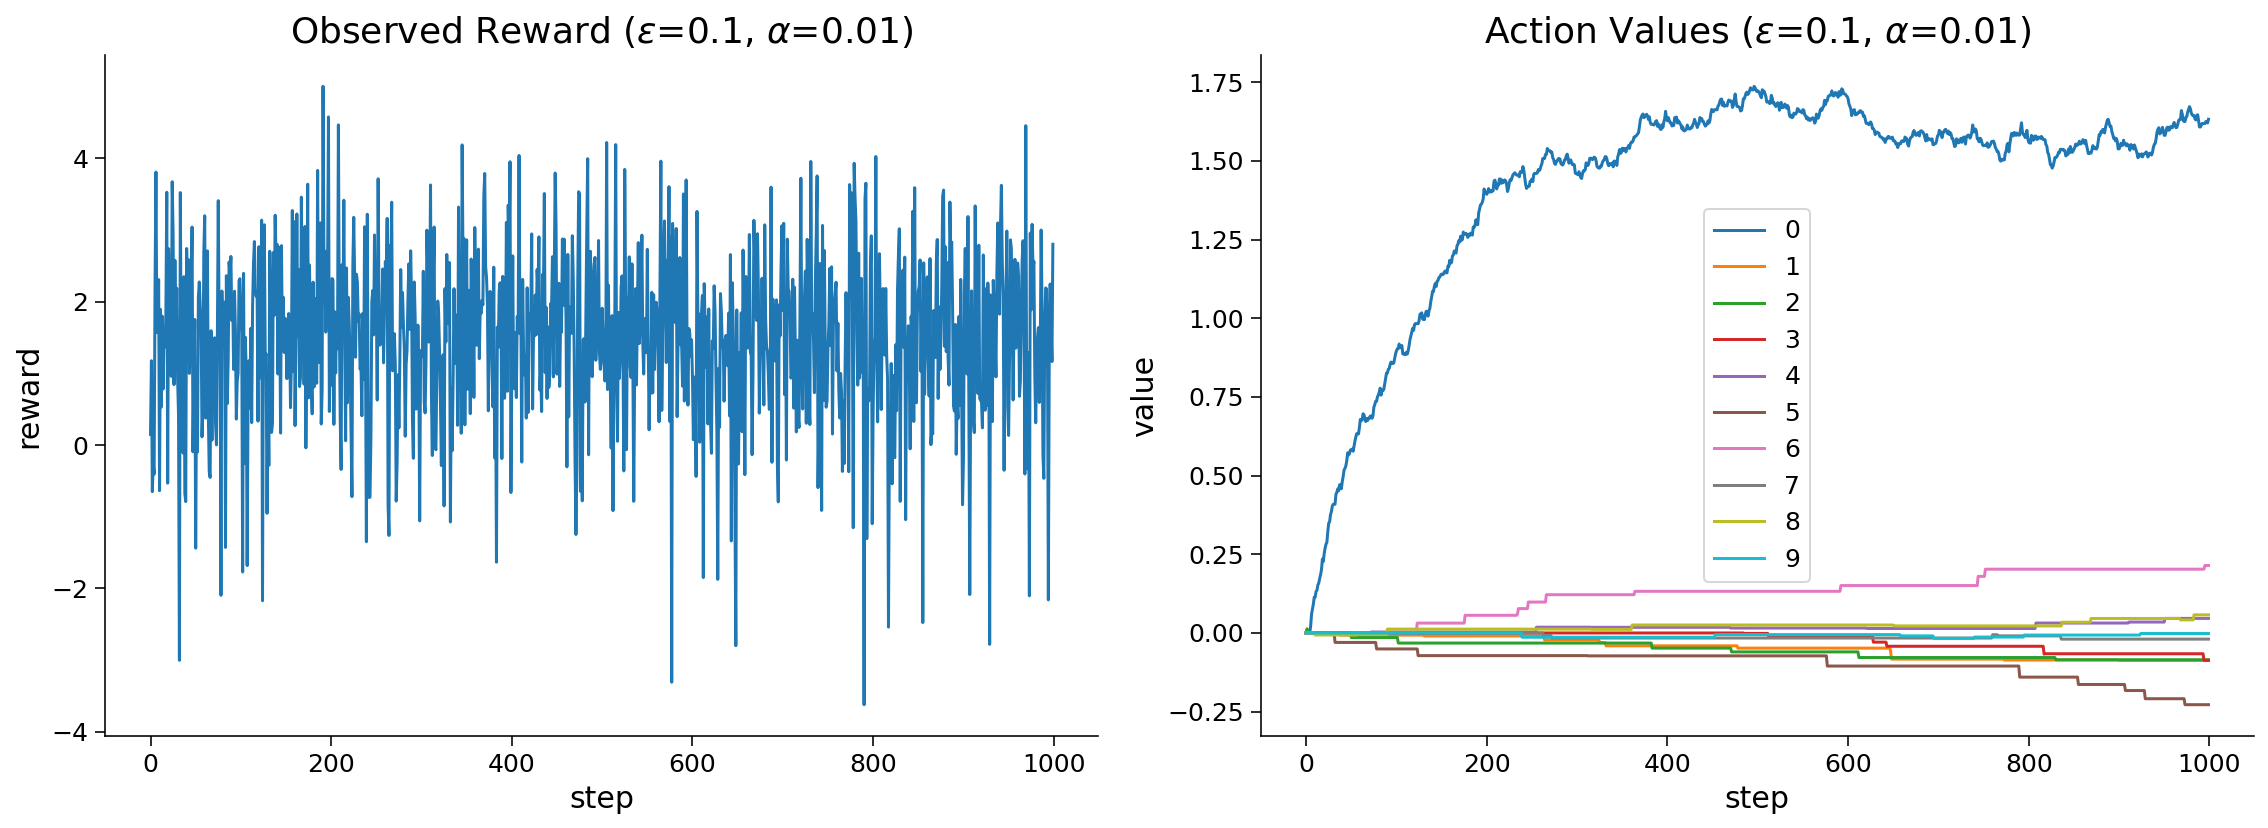
\includegraphics[scale=0.15]{Figures/RL/RL_Figure9.png}
\end{center}

Alright, we got some rewards that are kind of all over the place, but the agent seemed to settle in on the first arm as the preferred choice of action relatively quickly. Let's see how well we did at recovering the true means of the Gaussian random variables behind the arms.
\begin{center}
    
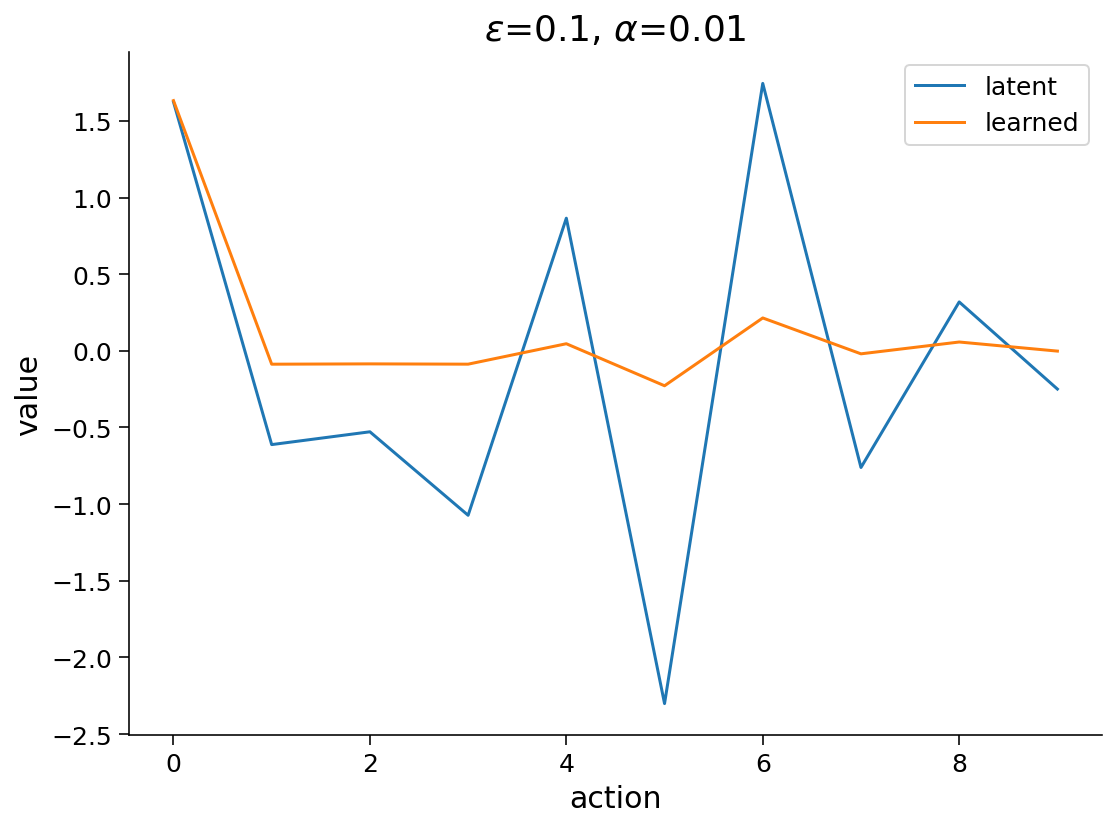
\includegraphics[scale=0.15]{Figures/RL/RL_Figure10.png}
\end{center}


Well, we seem to have found a very good estimate for action 0, but most of the others are not great. In fact, we can see the effect of the local maxima trap at work -- the greedy part of our algorithm locked onto action 0, which is actually the 2nd best choice to action 6. Since these are the means of Gaussian random variables, we can see that the overlap between the two would be quite high, so even if we did explore action 6, we may draw a sample that is still lower than our estimate for action 0.

However, this was just one choice of parameters. Perhaps there is a better combination?

\end{subbox}
\end{textbox}
%%%%%%%%%%%%%%%%%%%%%%%%%%%%%%%%%%%%%%%%%%%%%%%%%%%%%%
%%%%%%%%%%%%%%%%%%%%%%%%%%%%%%%%%%%%%%%%%%%%%%%%%%%%%%
\begin{textbox}{\href{https://compneuro.neuromatch.io/tutorials/W3D4_ReinforcementLearning/student/W3D4_Tutorial2.html}{Learning to Act: Multi-Armed Bandits } }

\begin{subbox}{subbox}{Changing Epsilon and Alpha}
\scriptsize
By varying the values of $\epsilon$ (exploitation-exploration tradeoff), $\alpha$ (learning rate), and even the number of actions $k$, changes the behavior of our agent.


\begin{center}
    
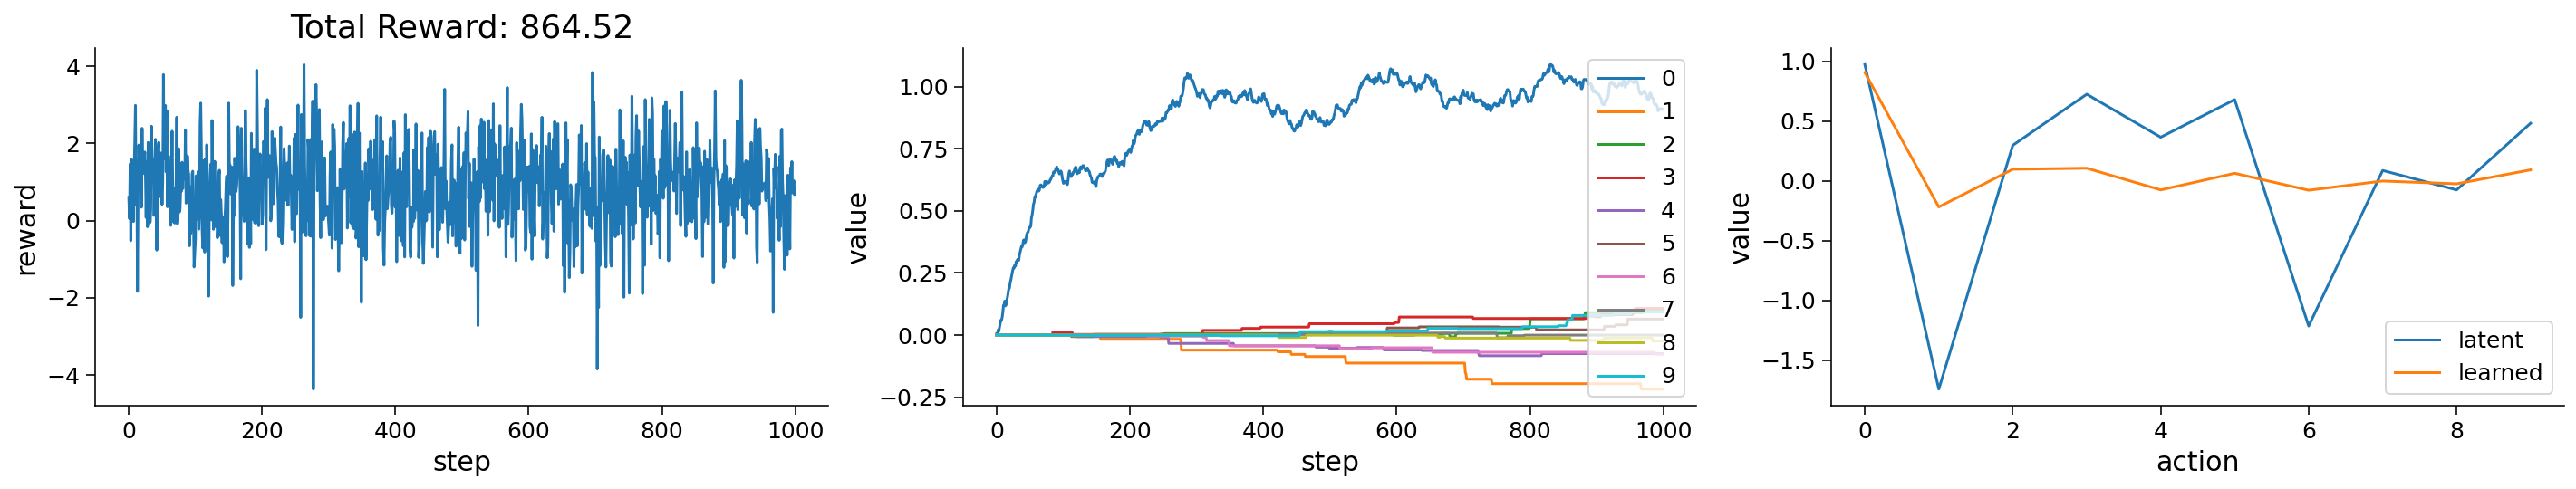
\includegraphics[scale=0.13]{Figures/RL/RL_Figure11.png}
\end{center}

While we can see how changing the $\epsilon$ and $\alpha$ values impact the agent's behavior, this doesn't give us a great sense of which combination is optimal. Due to the stochastic nature of both our rewards and our policy, a single trial run isn't sufficient to give us this information. Let's run multiple trials and compare the average performance.

First we will look at different values for $\epsilon \in [0.0, 0.1, 0.2]$ to a fixed $\alpha=0.1$. We will run 200 trials as a nice balance between speed and accuracy.

\begin{center}
    
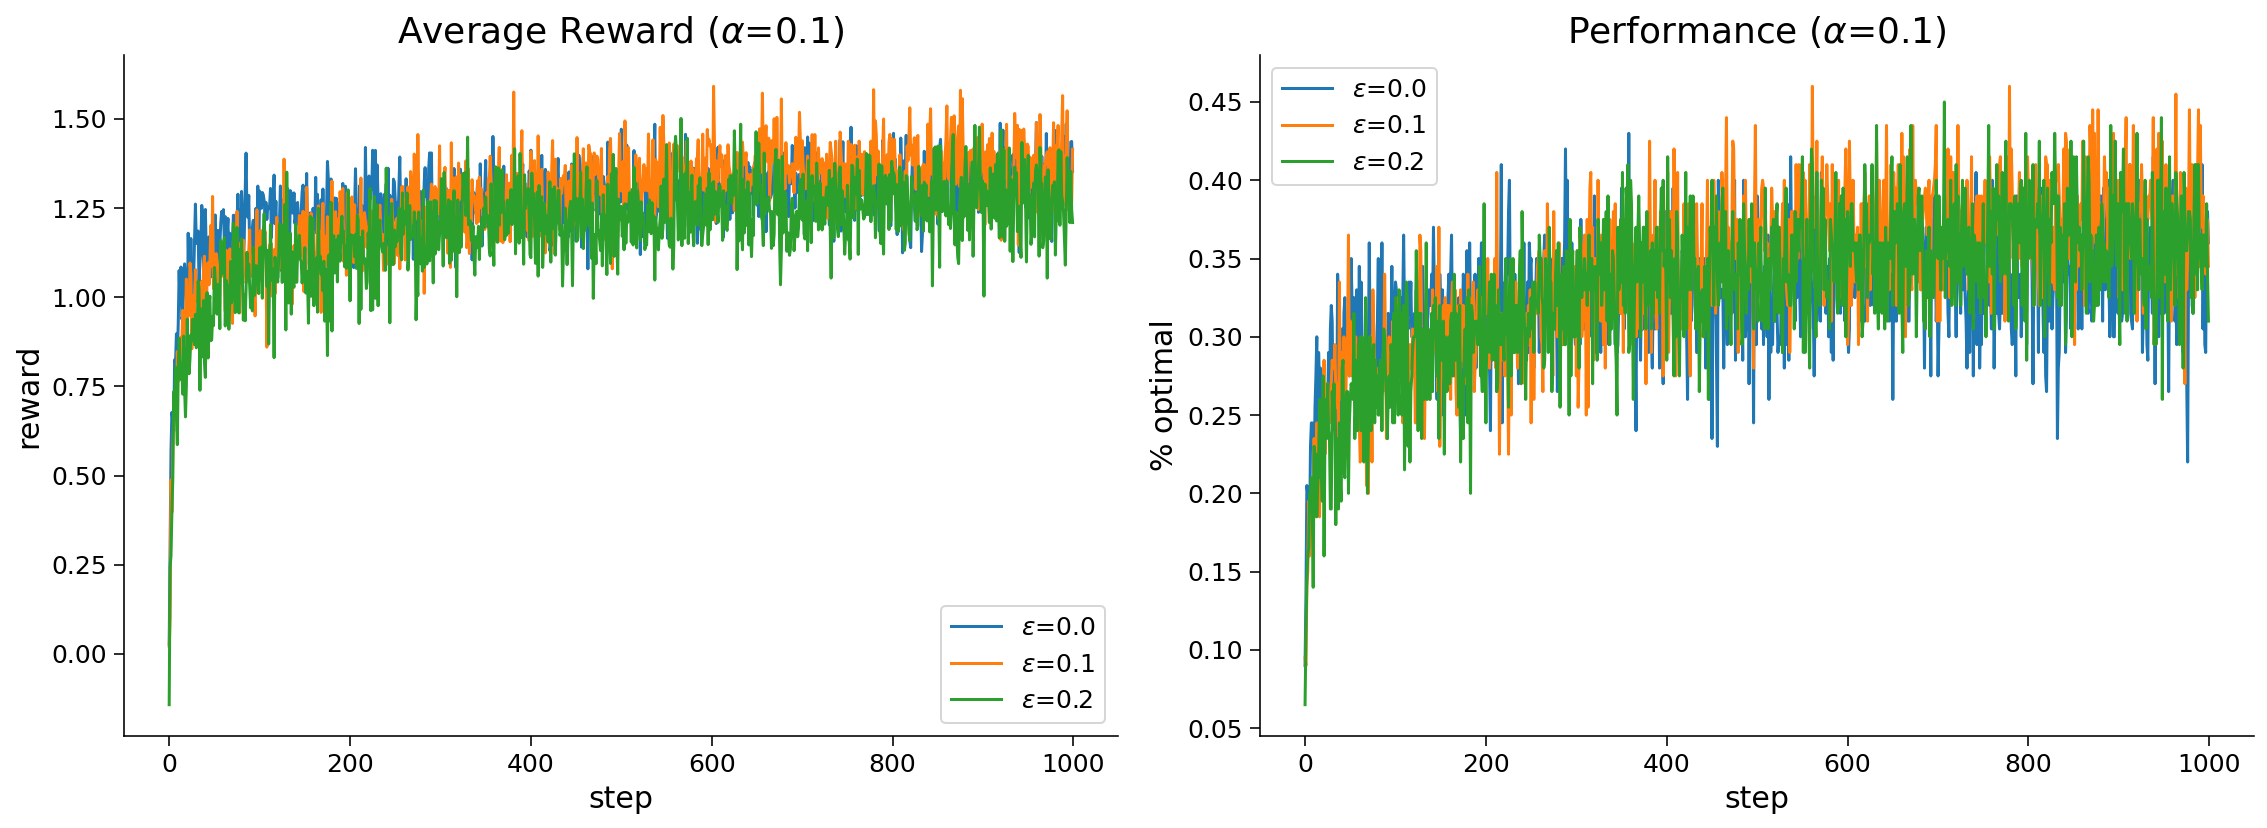
\includegraphics[scale=0.15]{Figures/RL/RL_Figure12.png}
\end{center}
On the left we have plotted the average reward over time, and we see that while $\epsilon=0$ (the greedy policy) does well initially, $\epsilon=0.1$ starts to do slightly better in the long run, while $\epsilon=0.2$ does the worst. Looking on the right, we see the percentage of times the optimal action (the best possible choice at time $t$) was taken, and here again we see a similar pattern of $\epsilon=0.1$ starting out a bit slower but eventually having a slight edge in the longer run.

We can also do the same for the learning rates. We will evaluate $\alpha \in [0.01, 0.1, 1.0]$ to a fixed $\epsilon=0.1$.

\begin{center}
    
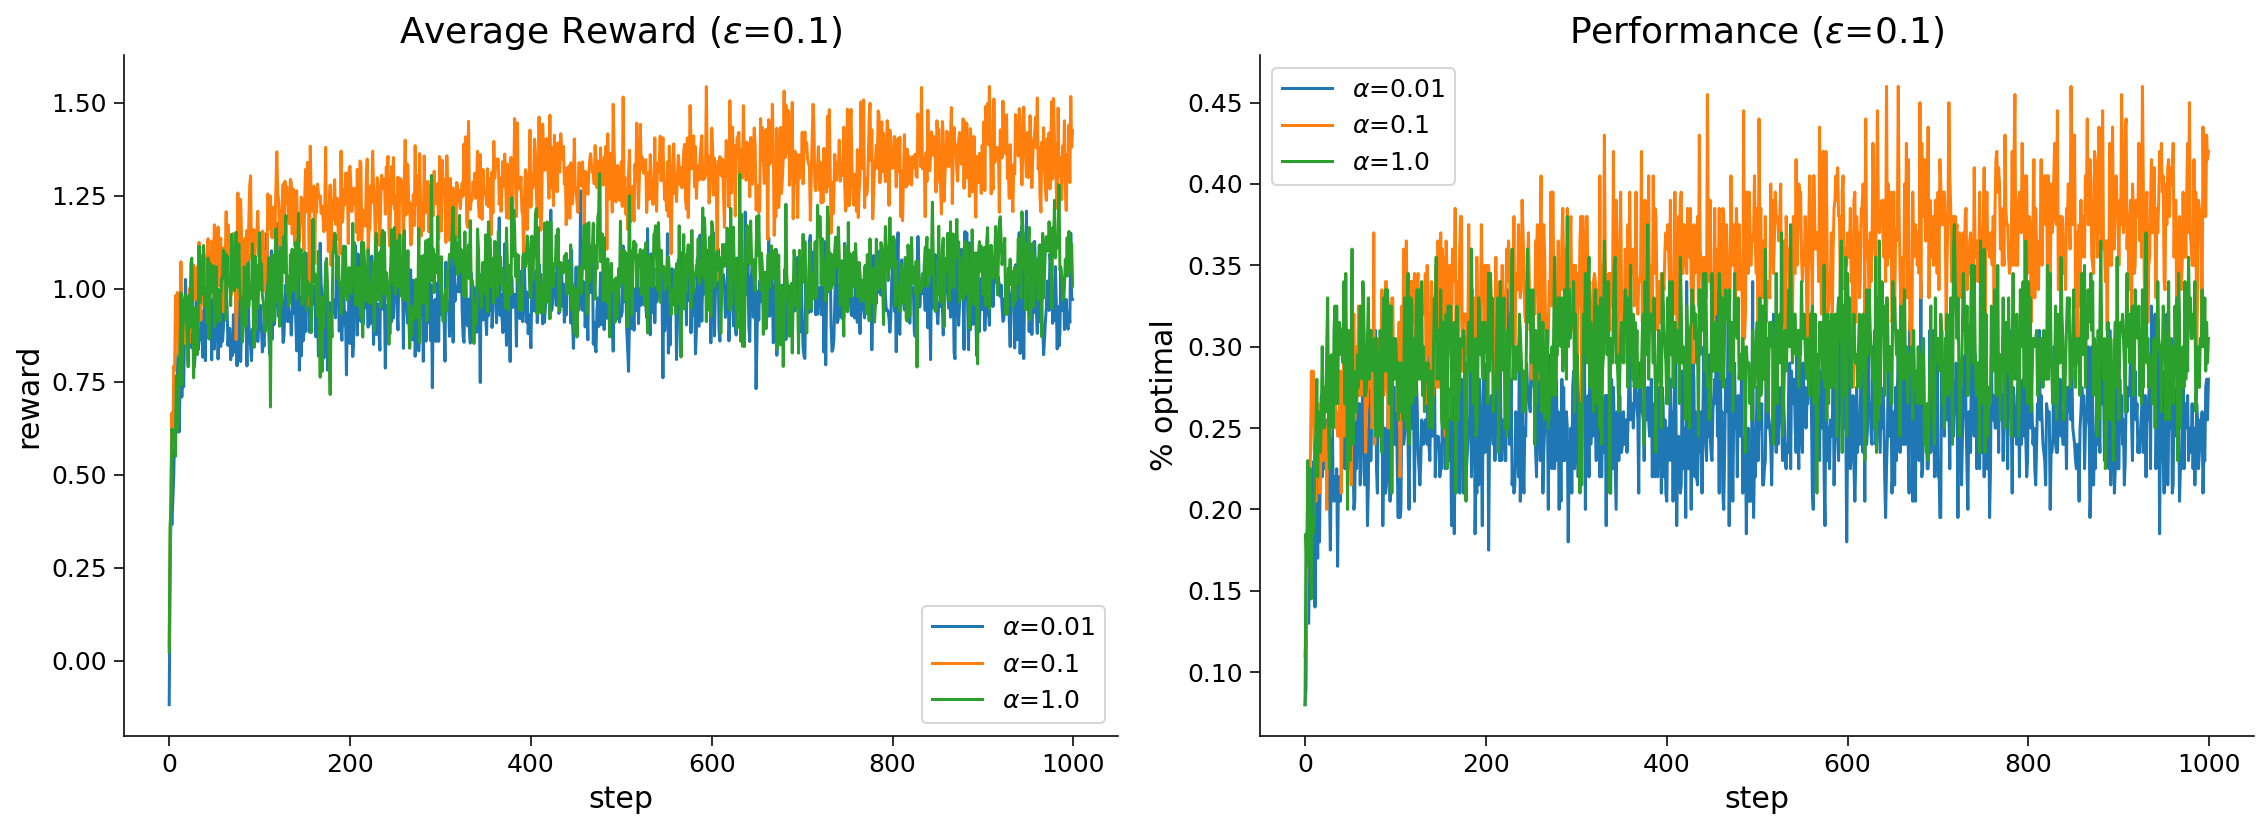
\includegraphics[scale=0.15]{Figures/RL/RL_Figure13.png}
\end{center}
Again we see a balance between an effective learning rate. $\alpha=0.01$ is too weak to quickly incorporate good values, while $\alpha=1$ is too strong likely resulting in high variance in values due to the Gaussian nature of the rewards.

\end{subbox}
\end{textbox}
\newpage
%%%%%%%%%%%%%%%%%%%%%%%%%%%%%%%%%%%%%%%%%%%%%%%%%%%%%%
%%%%%%%%%%%%%%%%%%%%%%%%%%%%%%%%%%%%%%%%%%%%%%%%%%%%%%
%%% TUTORIAL 3
%%%%%%%%%%%%%%%%%%%%%%%%%%%%%%%%%%%%%%%%%%%%%%%%%%%%%%
%%%%%%%%%%%%%%%%%%%%%%%%%%%%%%%%%%%%%%%%%%%%%%%%%%%%%%
\begin{textbox}{\href{https://compneuro.neuromatch.io/tutorials/W3D4_ReinforcementLearning/student/W3D4_Tutorial3.html}{Learning to Act: Q-Learning } }

\begin{subbox}{subbox}{Overview}
\scriptsize
Here you will learn how to act in the more realistic setting of sequential decisions, formalized by Markov Decision Processes (MDPs). In a sequential decision problem, the actions executed in one state not only may lead to immediate rewards (as in a bandit problem), but may also affect the states experienced next (unlike a bandit problem). Each individual action may therefore affect all future rewards. Thus, making decisions in this setting requires considering each action in terms of their expected \textbf{cumulative} future reward.

We will consider here the example of spatial navigation, where actions (movements) in one state (location) affect the states experienced next, and an agent might need to execute a whole sequence of actions before a reward is obtained.


\end{subbox}

\begin{subbox}{subbox}{Markov Decision Processes}
\scriptsize
\textbf{Grid Worlds}\\

As pointed out, bandits only have a single state and immediate rewards for our actions. Many problems we are interested in have multiple states and delayed rewards, i.e. we won't know if the choices we made will pay off over time, or which actions we took contributed to the outcomes we observed.

In order to explore these ideas, we turn to the common problem setting: the grid world. Grid worlds are simple environments where each state corresponds to a tile on a 2D grid, and the only actions the agent can take are to move up, down, left, or right across the grid tiles. The agent's job is almost always to find a way to a goal tile in the most direct way possible while overcoming some maze or other obstacles, either static or dynamic.

For our discussion we will be looking at the classic Cliff World, or Cliff Walker, environment. This is a $4 \times 10$ grid with a starting position in the lower-left and the goal position in the lower-right. Every tile between these two is the "cliff", and should the agent enter the cliff, they will receive a -100 reward and be sent back to the starting position. Every tile other than the cliff produces a -1 reward when entered. The goal tile ends the episode after taking any action from it.

\begin{center}
    
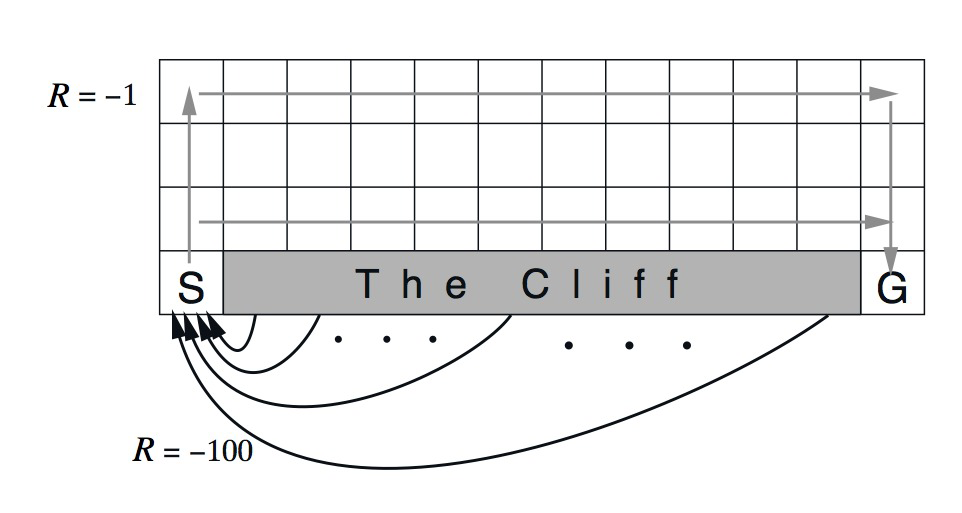
\includegraphics[scale=0.14]{Figures/RL/RL_Figure14.png}
\end{center}

Given these conditions, the maximum achievable reward is -11 (1 up, 9 right, 1 down). Using negative rewards is a common technique to encourage the agent to move and seek out the goal state as fast as possible.

\end{subbox}
\end{textbox}
%%%%%%%%%%%%%%%%%%%%%%%%%%%%%%%%%%%%%%%%%%%%%%%%%%%%%%
%%%%%%%%%%%%%%%%%%%%%%%%%%%%%%%%%%%%%%%%%%%%%%%%%%%%%%
\begin{textbox}{\href{https://compneuro.neuromatch.io/tutorials/W3D4_ReinforcementLearning/student/W3D4_Tutorial3.html}{Learning to Act: Q-Learning } }

\begin{subbox}{subbox}{Q-Learning}
\scriptsize

Now that we have our environment, how can we solve it? 

One of the most famous algorithms for estimating action values (aka Q-values) is the Temporal Differences (TD) control algorithm known as Q-learning (Watkins, 1989). 
\begin{eqnarray*}
Q(s_t,a_t) &\leftarrow& Q(s_t,a_t) + \\& & \alpha \big(r_t + \gamma\max_{\limits{a}} Q(s_{t+1},a_{t+1}) - Q(s_t,a_t)\big)
\end{eqnarray*}

where $Q(s,a)$ is the value function for action $a$ at state $s$, $\alpha$ is the learning rate, $r$ is the reward, and $\gamma$ is the temporal discount rate.

The expression $r_t + \gamma\max_{\limits{a}} Q(s_{t+1},a_{t+1})$ is referred to as the TD target while the full expression

\begin{equation}
r_t + \gamma\max_{\limits{a}} Q(s_{t+1},a_{t+1}) - Q(s_t,a_t),
\end{equation}

i.e., the difference between the TD target and the current Q-value, is referred to as the TD error, or reward prediction error.

Because of the max operator used to select the optimal Q-value in the TD target, Q-learning directly estimates the optimal action value, i.e., the cumulative future reward that would be obtained if the agent behaved optimally, regardless of the policy currently followed by the agent. For this reason, Q-learning is referred to as an \textbf{off-policy} method.


\end{subbox}

\begin{subbox}{subbox}{Implement the Q-learning algorithm}
\scriptsize



The top left is a representation of the Q-table itself, showing the values for different actions in different states. Notably, going right from the starting state or down when above the cliff is clearly very bad.\\
 The top right figure shows the greedy policy based on the Q-table, i.e. what action would the agent take if it only took its best guess in that state.\\
 The bottom right is the same as the top, only instead of showing the action, it's showing a representation of the maximum Q-value at a particular state.\\
 The bottom left is the actual proof of learning, as we see the total reward steadily increasing after each episode until asymptoting at the maximum possible reward of -11.

\begin{center}
    
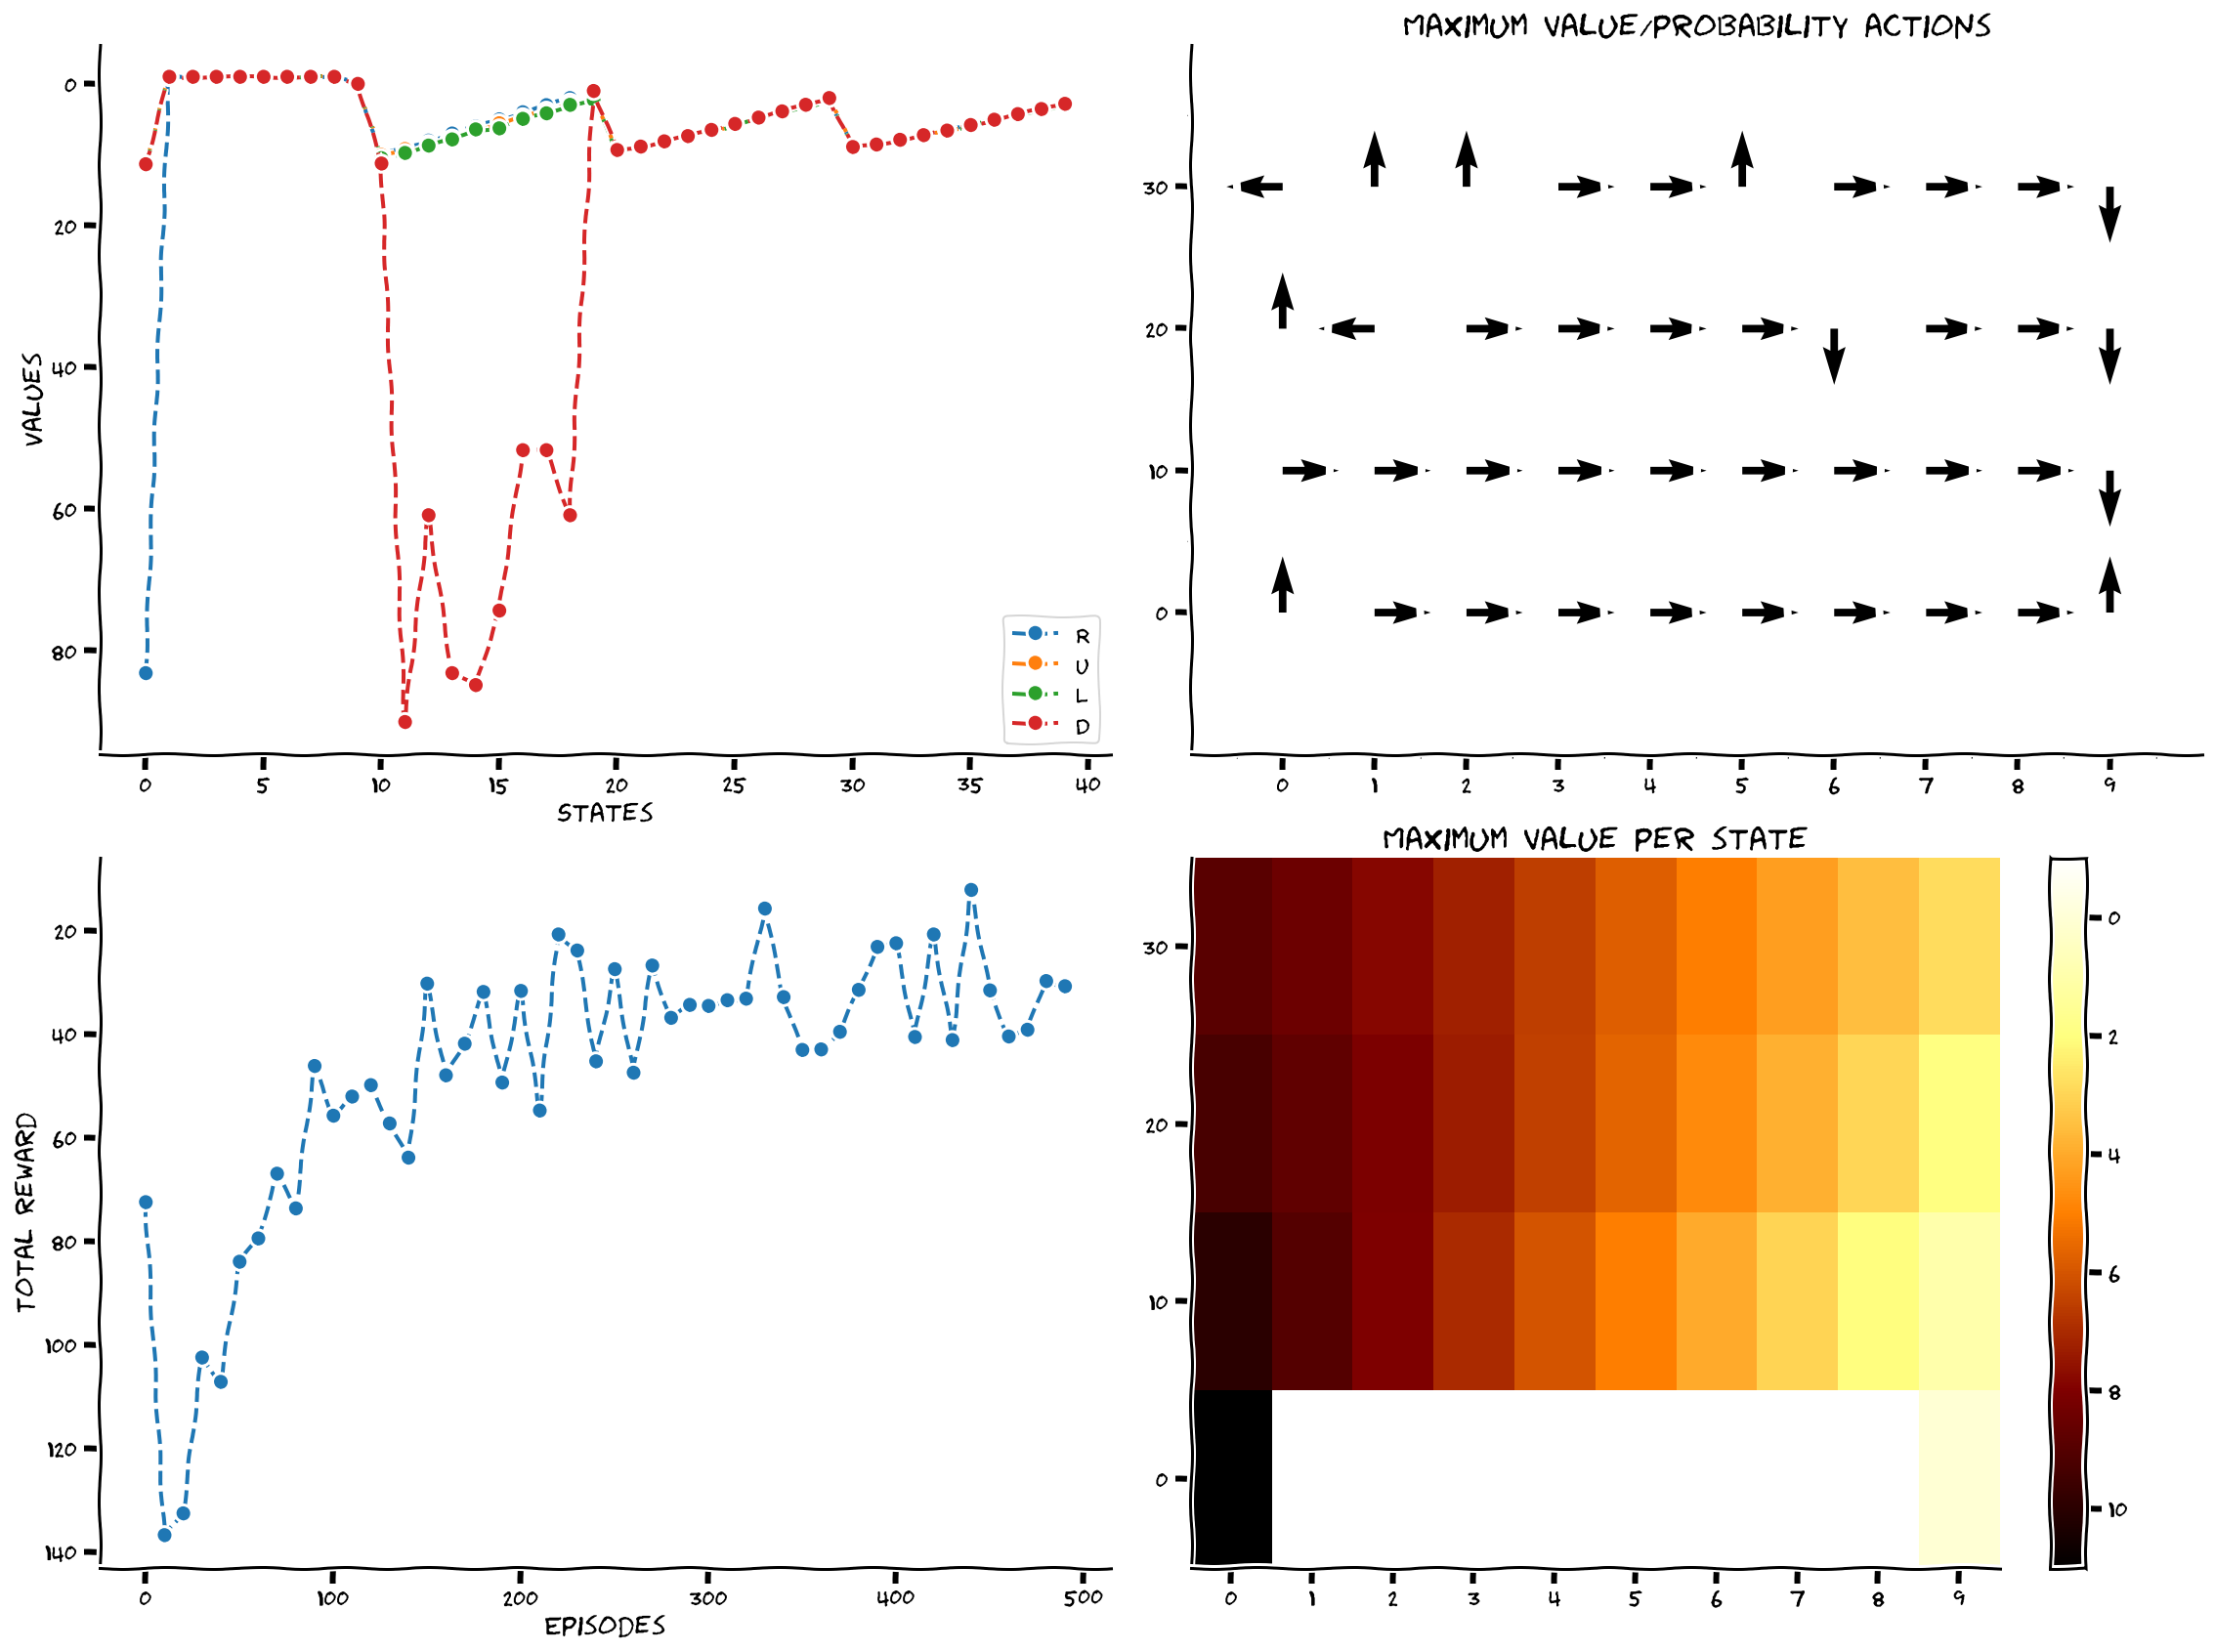
\includegraphics[scale=0.13]{Figures/RL/RL_Figure15.png}
\end{center}



\end{subbox}
\end{textbox}
\newpage
%%%%%%%%%%%%%%%%%%%%%%%%%%%%%%%%%%%%%%%%%%%%%%%%%%%%%%
%%%%%%%%%%%%%%%%%%%%%%%%%%%%%%%%%%%%%%%%%%%%%%%%%%%%%%
%%% TUTORIAL 4
%%%%%%%%%%%%%%%%%%%%%%%%%%%%%%%%%%%%%%%%%%%%%%%%%%%%%%
%%%%%%%%%%%%%%%%%%%%%%%%%%%%%%%%%%%%%%%%%%%%%%%%%%%%%%
\begin{textbox}{\href{https://compneuro.neuromatch.io/tutorials/W3D4_ReinforcementLearning/student/W3D4_Tutorial4.html}{From Reinforcement Learning to Planning } }

\begin{subbox}{subbox}{Model-based RL}
\scriptsize
The algorithms introduced in the previous tutorials are all *model-free*, as they do not require a model to use or control behavior. In this section, we will study a different class of algorithms called model-based. As we will see next, in contrast to model-free RL, model-based methods use a model to build a policy.

But what is a model? A model (sometimes called a world model or internal model) is a representation of how the world will respond to the agent's actions. You can think of it as a representation of how the world \textit{works}. With such a representation, the agent can simulate new experiences and learn from these simulations. This is advantageous for two reasons. First, acting in the real world can be costly and sometimes even dangerous. Learning from simulated experience can avoid some of these costs or risks. Second, simulations make fuller use of one's limited experience. To see why, imagine an agent interacting with the real world. The information acquired with each individual action can only be assimilated at the moment of the interaction. In contrast, the experiences simulated from a model can be simulated multiple times -- and whenever desired -- allowing for the information to be more fully assimilated.

Our RL agent will act in the Quentin's world, a 10x10 grid world. 
\begin{center}
    
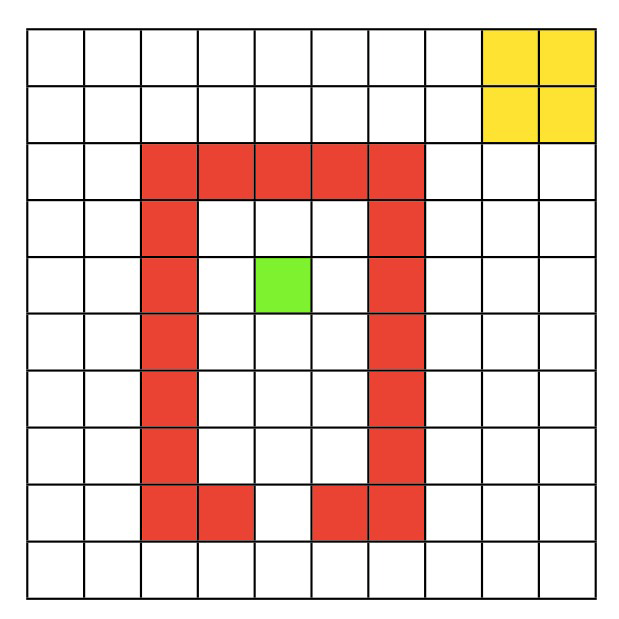
\includegraphics[scale=0.14]{Figures/RL/RL_Figure16.png}
\end{center}
In this environment, there are 100 states and 4 possible actions: right, up, left, and down. The goal of the agent is to move, via a series of steps, from the start (green) location to the goal (yellow) region, while avoiding the red walls. More specifically:
\begin{itemize}
    \item 
 The agent starts in the green state,
\item Moving into one of the red states incurs a reward of -1,
\item Moving into the world borders stays in the same place,
\item Moving into the goal state (yellow square in the upper right corner) gives you a reward of 1, and
\item Moving anywhere from the goal state ends the episode.
\end{itemize}

Now that we have our environment and task defined, how can we solve this using a model-based RL agent?

\end{subbox}

\end{textbox}
%%%%%%%%%%%%%%%%%%%%%%%%%%%%%%%%%%%%%%%%%%%%%%%%%%%%%%
%%%%%%%%%%%%%%%%%%%%%%%%%%%%%%%%%%%%%%%%%%%%%%%%%%%%%%
\begin{textbox}{\href{https://compneuro.neuromatch.io/tutorials/W3D4_ReinforcementLearning/student/W3D4_Tutorial4.html}{From Reinforcement Learning to Planning } }

\begin{subbox}{subbox}{ Dyna-Q}
\scriptsize
In this section, we will implement Dyna-Q, one of the simplest model-based reinforcement learning algorithms. A Dyna-Q agent combines acting, learning, and planning. The first two components -- acting and learning -- are just like what we have studied previously. Q-learning, for example, learns by acting in the world, and therefore combines acting and learning. But a Dyna-Q agent also implements planning, or simulating experiences from a model--and learns from them. 

In theory, one can think of a Dyna-Q agent as implementing acting, learning, and planning simultaneously, at all times. But, in practice, one needs to specify the algorithm as a sequence of steps. The most common way in which the Dyna-Q agent is implemented is by adding a planning routine to a Q-learning agent: after the agent acts in the real world and learns from the observed experience, the agent is allowed a series of $k$ *planning steps*. At each one of those $k$ planning steps, the model generates a simulated experience by randomly sampling from the history of all previously experienced state-action pairs. The agent then learns from this simulated experience, again using the same Q-learning rule that you implemented for learning from real experience. This simulated experience is simply a one-step transition, i.e., a state, an action, and the resulting state and reward. So, in practice, a Dyna-Q agent learns (via Q-learning) from one step of \textbf{real} experience during acting, and then from k steps of \textbf{simulated} experience during planning.

There's one final detail about this algorithm: where does the simulated experiences come from or, in other words, what is the "model"? In Dyna-Q, as the agent interacts with the environment, the agent also learns the model. For simplicity, Dyna-Q implements model-learning in an almost trivial way, as simply caching the results of each transition. Thus, after each one-step transition in the environment, the agent saves the results of this transition in a big matrix, and consults that matrix during each of the planning steps. Obviously, this model-learning strategy only makes sense if the world is deterministic (so that each state-action pair always leads to the same state and reward), and this is the setting of the exercise below. However, even this simple setting can already highlight one of Dyna-Q major strengths: the fact that the planning is done at the same time as the agent interacts with the environment, which means that new information gained from the interaction may change the model and thereby interact with planning in potentially interesting ways.

\end{subbox}
\end{textbox}
%%%%%%%%%%%%%%%%%%%%%%%%%%%%%%%%%%%%%%%%%%%%%%%%%%%%%%
%%%%%%%%%%%%%%%%%%%%%%%%%%%%%%%%%%%%%%%%%%%%%%%%%%%%%%
\begin{textbox}{\href{https://compneuro.neuromatch.io/tutorials/W3D4_ReinforcementLearning/student/W3D4_Tutorial4.html}{From Reinforcement Learning to Planning } }

\begin{subbox}{subbox}{Dyna-Q Algorithm}
\scriptsize

Initialize $Q(s,a)$ and $Model(s,a)$ for all $s \in S$ and $a \in A$.\\
Loop forever:\\
\begin{enumerate}[label=(\alph*)]
    \item 
 $S$ $\leftarrow$ current (nonterminal) state 
 \item  $A$ $\leftarrow$ $\epsilon$-greedy$(S,Q)$ 
   \item  Take action $A$; observe resultant reward, $R$, and state, $S'$ 
   \item  $Q(S,A)\leftarrow Q(S,A) + \alpha \left[R + \gamma \max_{a} Q(S',a) - Q(S,A)\right]$ 
   \item  $Model(S,A)$ $\leftarrow$ $R,S'$ (assuming deterministic environment) 
   \item  Loop repeat $k$ times: 
 $S$ $\leftarrow$ random previously observed state \\
 $A$ $\leftarrow$ random action previously taken in $S$ \\
 $R,S'$ $\leftarrow$ $Model(S,A)$ \\
 $Q(S,A) \leftarrow Q(S,A) + \alpha \left[R + \gamma \max_{a} Q(S',a) - Q(S,A)\right]$ 
\end{enumerate}

\end{subbox}

\begin{subbox}{subbox}{Implementing Dyna-Q}
\scriptsize

The plot below show an implementation of Dyna-Q  planning to try and solve Quentin's World. Notice that we set the number of planning steps $k=10$.
\begin{center}
    
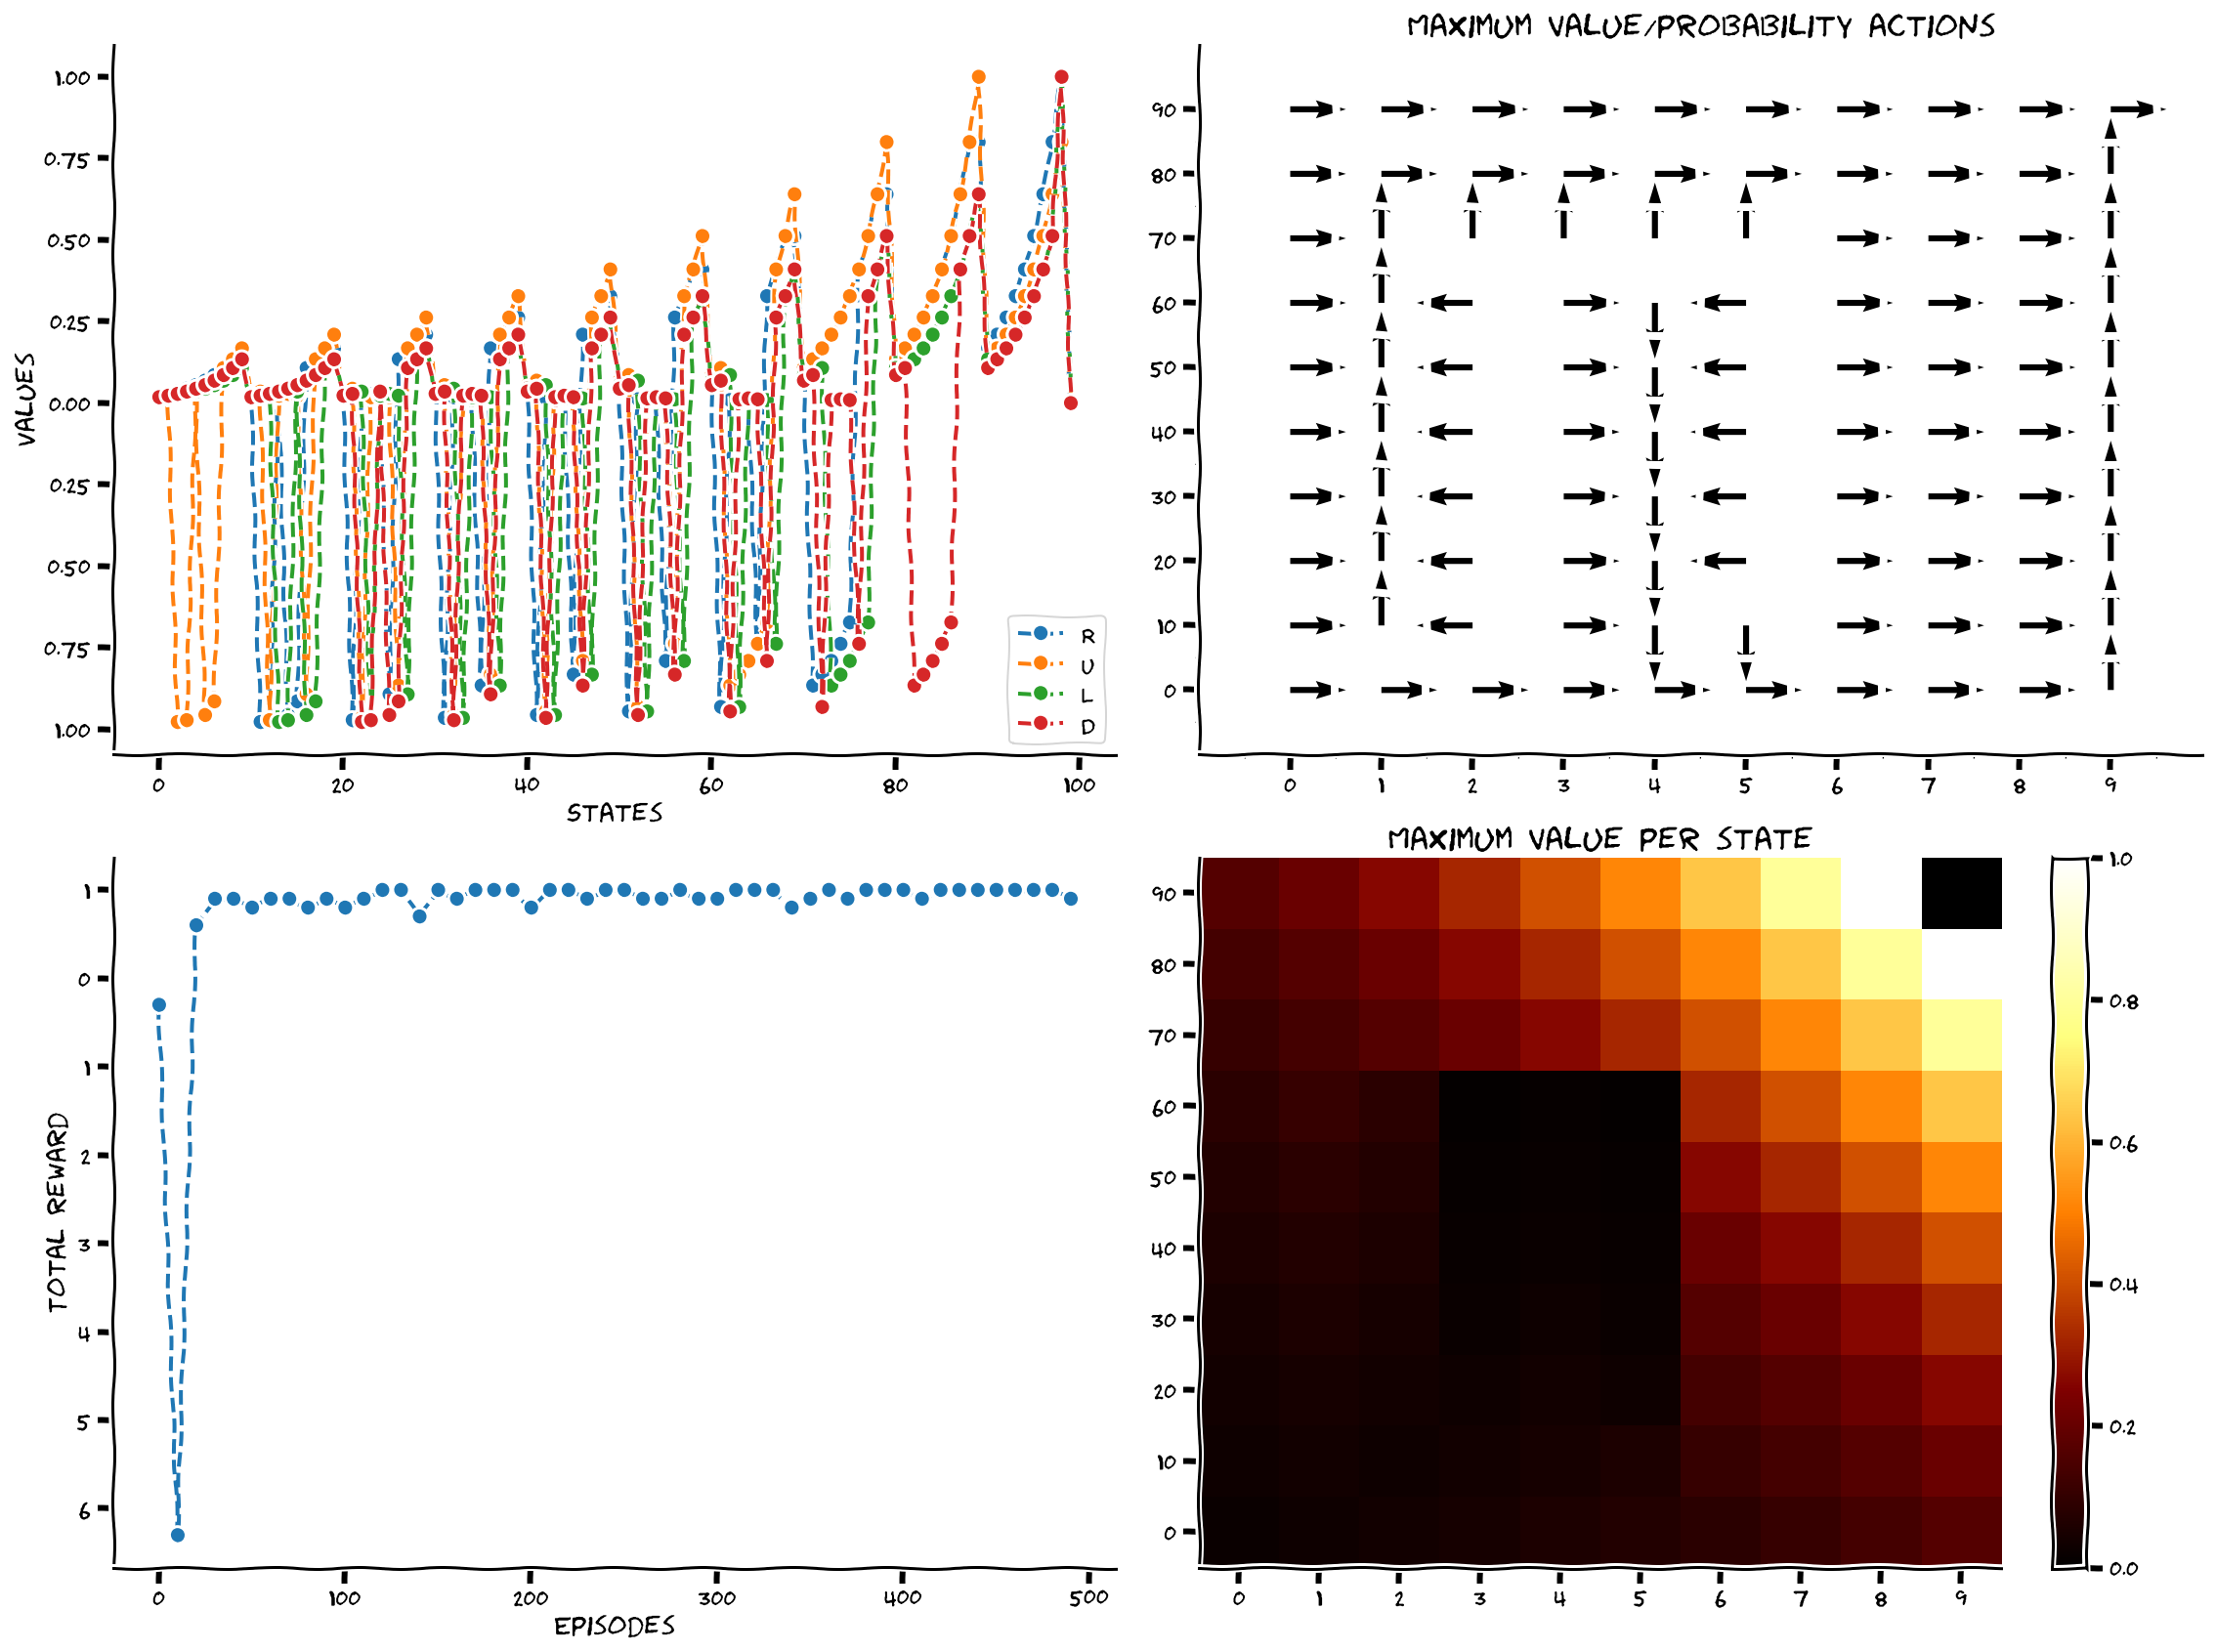
\includegraphics[scale=0.16]{Figures/RL/RL_Figure17.png}
\end{center}

The Dyna-Q agent is able to solve the task quite quickly, achieving a consistent positive reward after only a limited number of episodes (bottom left).

\end{subbox}
\end{textbox}
%%%%%%%%%%%%%%%%%%%%%%%%%%%%%%%%%%%%%%%%%%%%%%%%%%%%%%
%%%%%%%%%%%%%%%%%%%%%%%%%%%%%%%%%%%%%%%%%%%%%%%%%%%%%%
\begin{textbox}{\href{https://compneuro.neuromatch.io/tutorials/W3D4_ReinforcementLearning/student/W3D4_Tutorial4.html}{From Reinforcement Learning to Planning } }

\begin{subbox}{subbox}{How much to plan?}
\scriptsize

We implemented a Dyna-Q agent with $k=10$, we will try to understand the effect of planning on performance. How does changing the value of $k$ impact our agent's ability to learn?

The following code is similar to what we just ran, only this time we run several experiments over several different values of $k$ to see how their average performance compares. In particular, we will choose $k \in \{0, 1, 10, 100\}$. Pay special attention to the case where $k = 0$ which corresponds to no planning. This is, in effect, just regular Q-learning.

The following code will take a bit of time to complete. To speed things up, try lowering the number of experiments or the number of $k$ values to compare.


\begin{center}
    
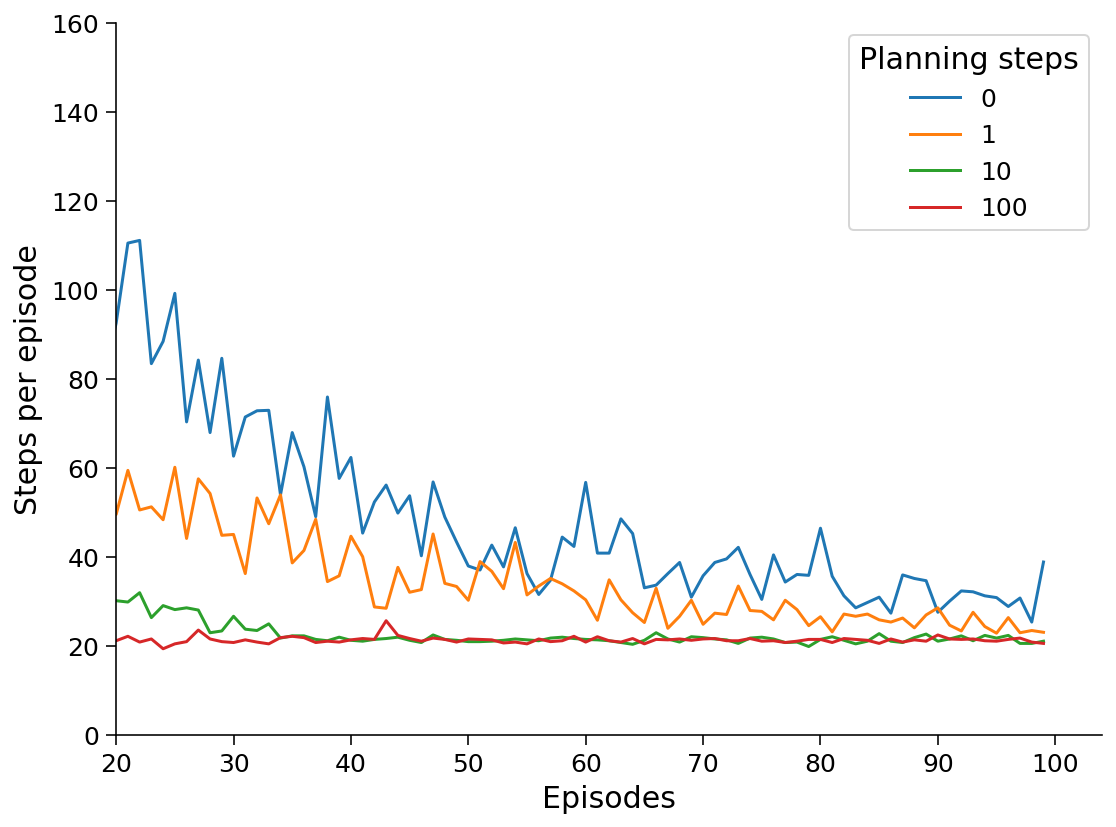
\includegraphics[scale=0.25]{Figures/RL/RL_Figure18.png}
\end{center}
After an initial warm-up phase of the first 20 episodes, we should see that the number of planning steps has a noticeable impact on our agent's ability to rapidly solve the environment. We should also notice that after a certain value of $k$ our relative utility goes down, so it's important to balance a large enough value of $k$ that helps us learn quickly without wasting too much time in planning.

\end{subbox}
\end{textbox}
%%%%%%%%%%%%%%%%%%%%%%%%%%%%%%%%%%%%%%%%%%%%%%%%%%%%%%
%%%%%%%%%%%%%%%%%%%%%%%%%%%%%%%%%%%%%%%%%%%%%%%%%%%%%%
\begin{textbox}{\href{https://compneuro.neuromatch.io/tutorials/W3D4_ReinforcementLearning/student/W3D4_Tutorial4.html}{From Reinforcement Learning to Planning } }
\begin{subbox}{subbox}{When the world changes...}
\scriptsize

In addition to speeding up learning about a new environment, planning can also help the agent to quickly incorporate new information about the environment into its policy. Thus, if the environment changes (e.g. the rules governing the transitions between states, or the rewards associated with each state/action), the agent doesn't need to experience that change *repeatedly* (as would be required in a Q-learning agent) in real experience. Instead, planning allows that change to be incorporated quickly into the agent's policy, without the need to experience the change more than once.

In this final section, we will again have our agents attempt to solve Quentin's World. However, after 200 episodes, a shortcut will appear in the environment.  We will test how a model-free agent using Q-learning and a Dyna-Q agent adapt to this change in the environment.

\begin{center}
    
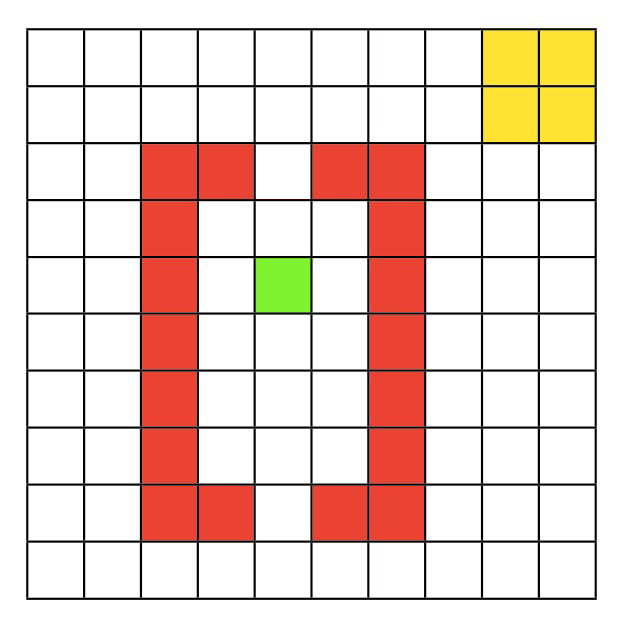
\includegraphics[scale=0.14]{Figures/RL/RL_Figure19.png}
\end{center}
The following code again looks similar to what we've run previously. Just as above we will have multiple values for $k$, with $k=0$ representing our Q-learning agent and $k=10$ for our Dyna-Q agent with 10 planning steps. The main difference is we now add in an indicator as to when the shortcut appears. In particular, we will run the agents for 400 episodes, with the shortcut appearing in the middle after episode #200.

When this shortcut appears we will also let each agent experience this change once i.e. we will evaluate the act of moving upwards when in the state that is below the now-open shortcut. After this single demonstration, the agents will continue on interacting in the environment.
\begin{center}
    
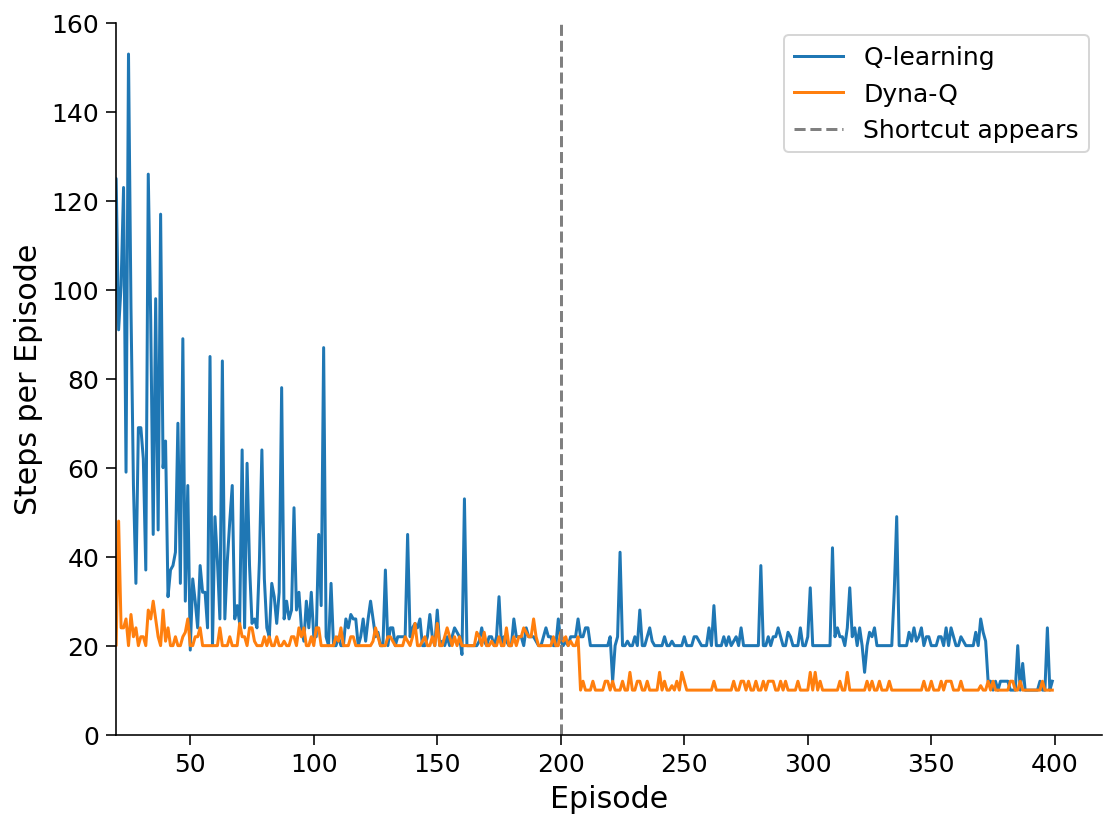
\includegraphics[scale=0.14]{Figures/RL/RL_Figure20.png}
\end{center}

If all went well, we should see the Dyna-Q agent having already achieved near optimal performance before the appearance of the shortcut and then immediately incorporating this new information to further improve. In this case, the Q-learning agent takes much longer to fully incorporate the new shortcut.


\end{subbox}
\end{textbox}
%%%%%%%%%%%%%%%%%%%%%%%%%%%%%%%%%%%%%%%%%%%%%%%%%%%%%%
%%%%%%%%%%%%%%%%%%%%%%%%%%%%%%%%%%%%%%%%%%%%%%%%%%%%%%
\begin{textbox}{\href{https://compneuro.neuromatch.io/tutorials/W3D4_ReinforcementLearning/student/W3D4_Tutorial4.html}{From Reinforcement Learning to Planning } }
\begin{subbox}{subbox}{Summary}
\scriptsize

In this notebook, you have learned about model-based reinforcement learning and implemented one of the simplest architectures of this type, Dyna-Q. Dyna-Q is very much like Q-learning, but instead of learning only from real experience, you also learn from **simulated** experience. This small difference, however, can have huge benefits! Planning *frees* the agent from the limitation of its own environment, and this in turn allows the agent to speed-up learning -- for instance, effectively incorporating environmental changes into one's policy.

Not surprisingly, model-based RL is an active area of research in machine learning. Some of the exciting topics in the frontier of the field involve (i) learning and representing a complex world model (i.e., beyond the tabular and deterministic case above), and (ii) what to simulate -- also known as search control -- (i.e., beyond the random selection of experiences implemented above).

The framework above has also been used in neuroscience to explain various phenomena such as planning, memory sampling, memory consolidation, and even dreaming!

\end{subbox}
\end{textbox}
\end{multicols}
\newpage
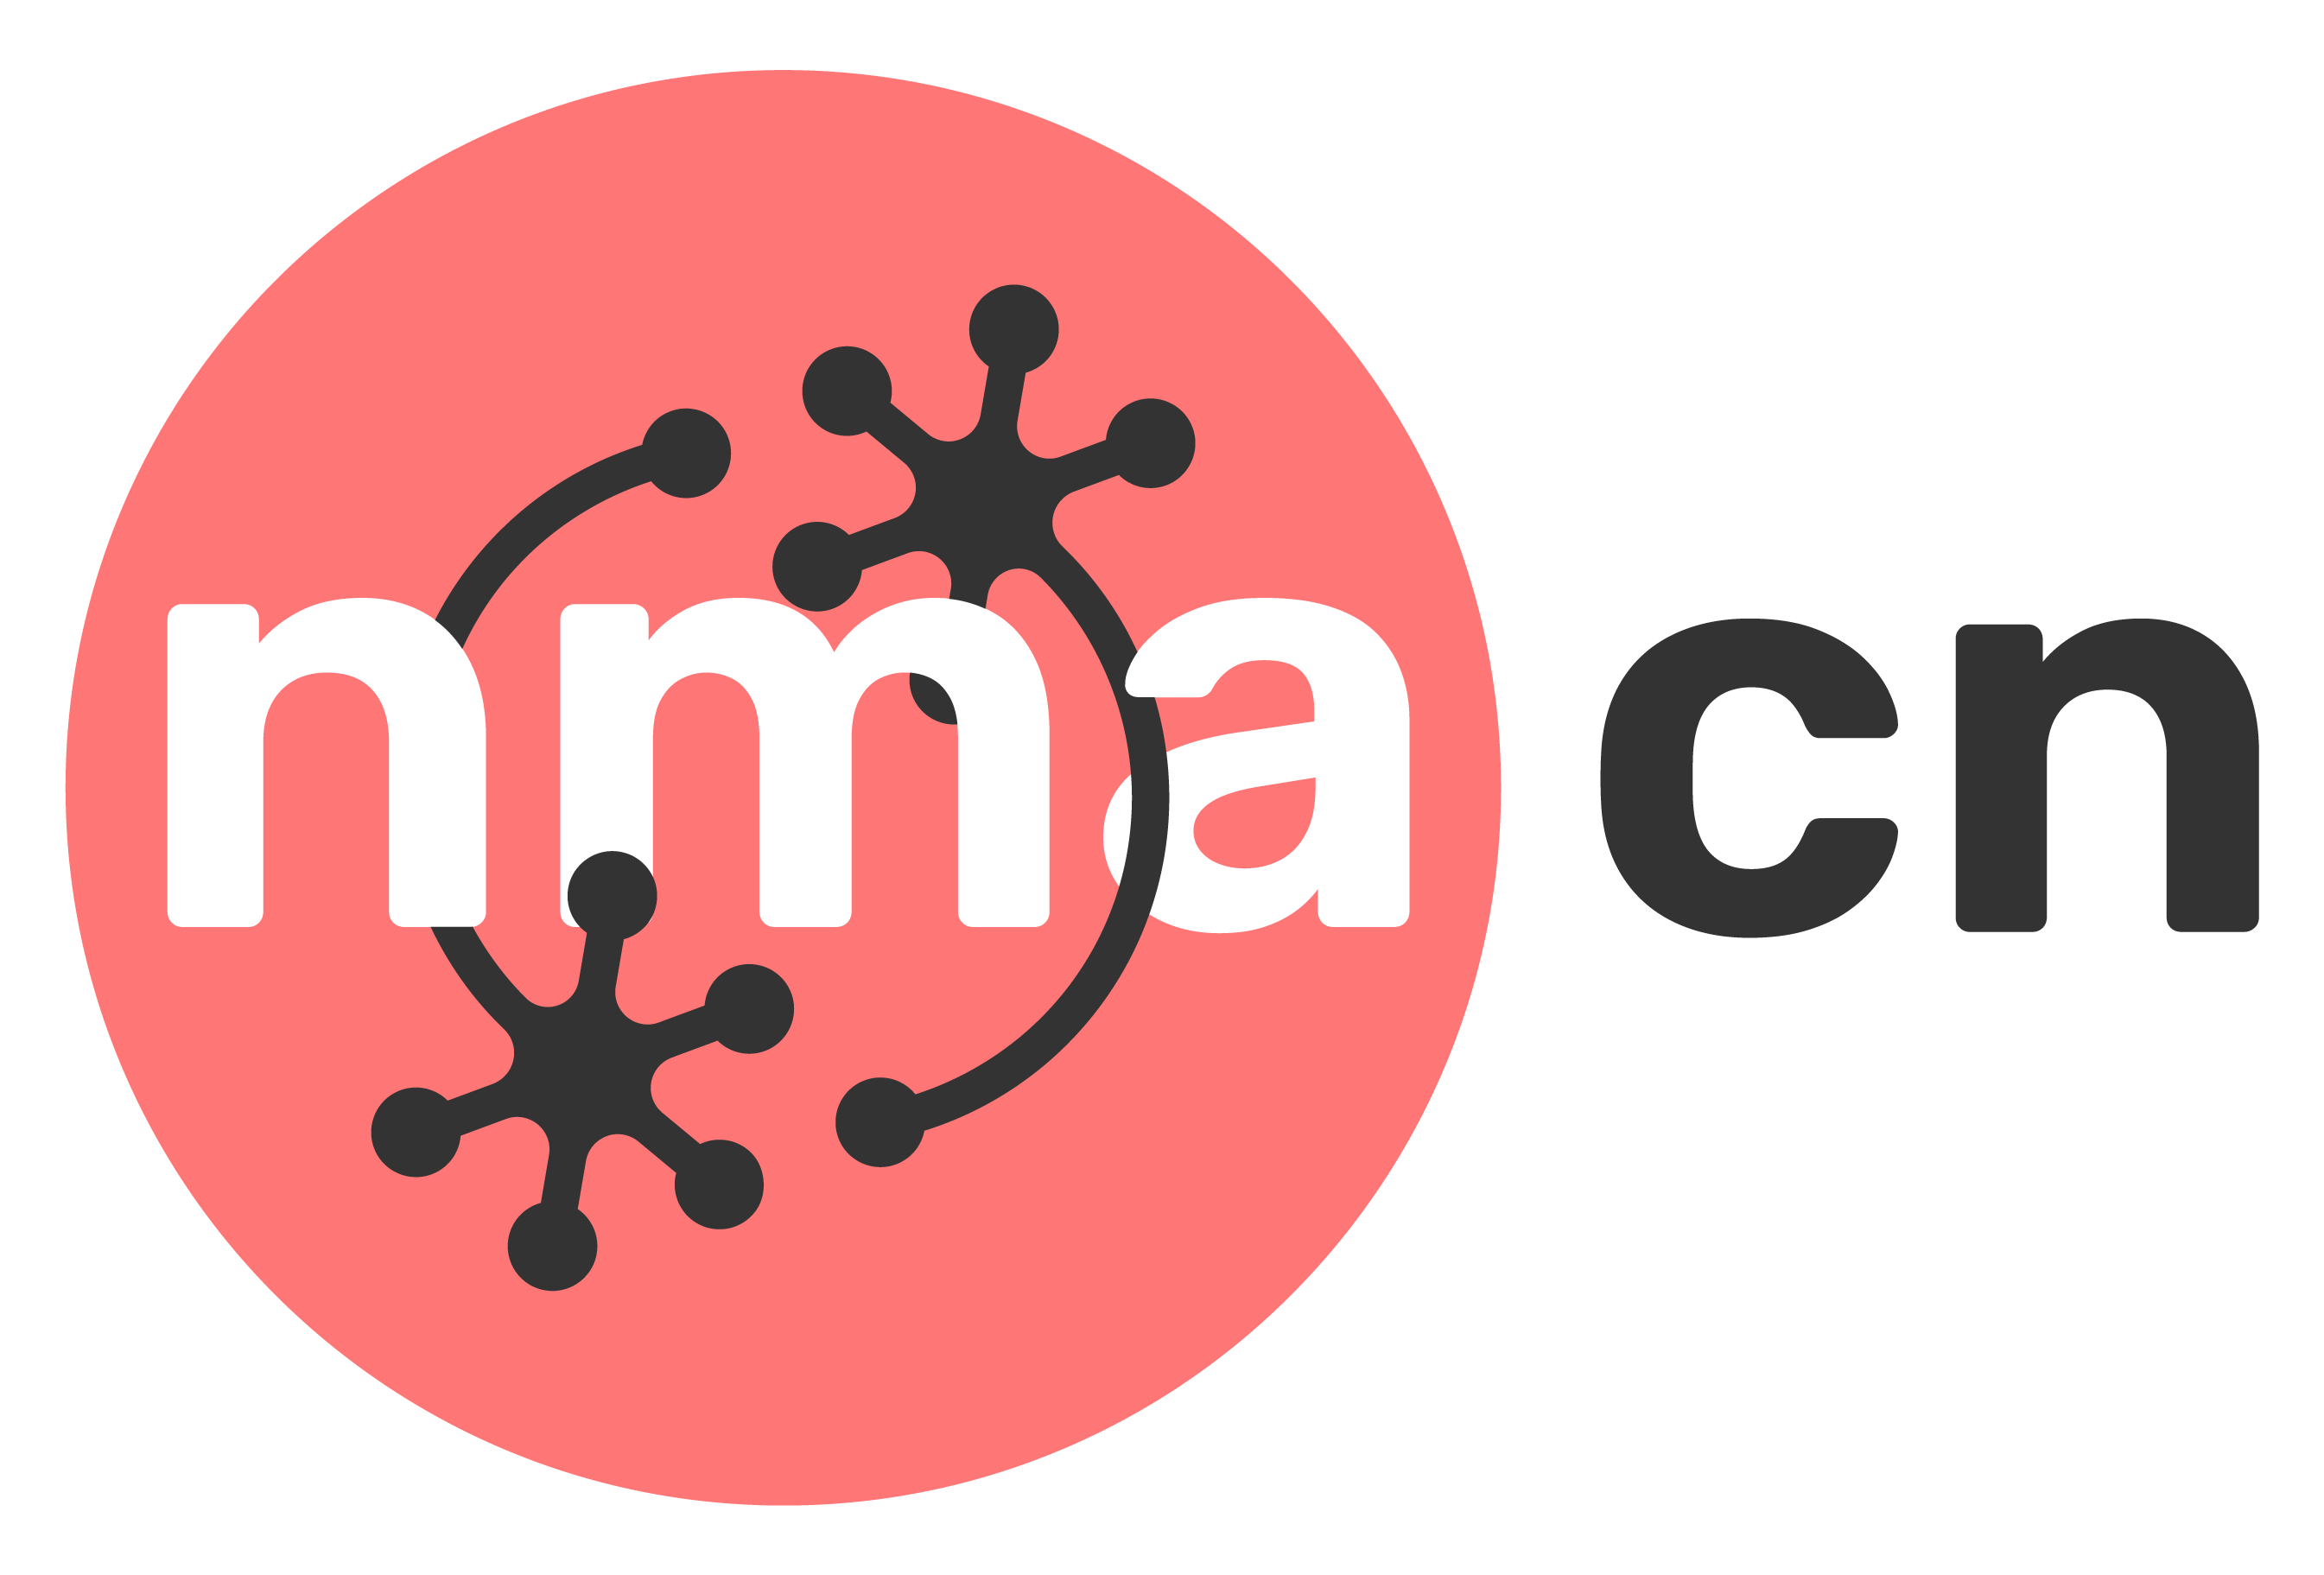
\includegraphics[scale=0.03]{Figures/NMACN.png}\href{https://compneuro.neuromatch.io/tutorials/intro.html}{\textbf{\Huge{Neuromatch Academy: Network Causality - Summary Sheet}}\footnote{’t Hart et al., (2022). Neuromatch Academy: a 3-week, online summer school in computational neuroscience. Journal of Open Source Education, 5(49), 118. https://doi.org/10.21105/jose.00118}}
%$\subsection*{Cheat Sheet}
\small

\begin{multicols}{3}

\let\clearpage\relax
\begin{textbox}{\href{https://compneuro.neuromatch.io/tutorials/W3D5_NetworkCausality/student/W3D5_Tutorial1.html}{Interventions (W3D5T1)}   }
\begin{subbox}{subbox}{Overview}
\scriptsize
Here we will describe causality, the tools we use to ask if and how a variable influences other variables. Causal questions are everywhere in neuroscience. How do neurons influence one another? How does a drug affect neurons? How does a stimulus affect behavior? We will talk about how we can answer questions of a causal kind. 
Causal questions are important all across neuroscience. For example, model fitting, machine learning, and dimensionality reduction, are often used to argue for or against causal models. For example, a regression may be used to argue that a brain region influences another brain region based on fMRI data. Today’s materials give us a better understanding of the problems that come with the approach. There are tight links between causality and Bayesian statistics where Bayesian techniques are used for the estimation of causality (see e.g. the work of Judea Pearl). Causality is often seen as the bedrock of science, today’s materials above all produce clarity about what it is.

Causality approaches are central across neuroscience. When we run experiments, we often randomly assign them to treatment groups vs control. Alternatively we stimulate animals at random points of time. These methods are all versions of randomized perturbations  and probably constitute a good part of all of neuroscience. We also use model fitting  frequently to drive arguments about how brains work. This is common for spike data, EEG data, imaging data etc. Lastly, we should be able to sometimes use instrumental variable techniques to estimate the effects of e.g. treatments with drugs. These materials are simultaneously at the heart of the field and are frequently ignored.

\end{subbox}
\end{textbox}
%%%%%%%%%%%%%%%%%%%%%%%%% 
%%%%%%%%%%%%%%%%%%%%%%%%%
\begin{textbox}{\href{https://compneuro.neuromatch.io/tutorials/W3D5_NetworkCausality/student/W3D5_Tutorial1.html}{Interventions (W3D5T1)}   }
\begin{subbox}{subbox}{Introduction}
\scriptsize
How do we know if a relationship is causal? What does that mean? And how can we estimate causal relationships within neural data?\\

The methods we'll learn today are very general and can be applied to all sorts of data, and in many circumstances.\\
Causal questions are everywhere!

\end{subbox}
\begin{subbox}{subbox}{Defining and estimating causality}
\scriptsize

Let's think carefully about the statement "\textbf{A causes B}". To be concrete, let's take two neurons. What does it mean to say that neuron $A$ causes neuron $B$ to fire?

The \textit{interventional} definition of causality says that:
\begin{eqnarray*}
(A \text{ causes } B) &\Leftrightarrow& ( \text{ If we force }A \\
& & \text { to be different, then }B\text{ changes})
\end{eqnarray*}

To determine if $A$ causes $B$ to fire, we can inject current into neuron $A$ and see what happens to $B$.\\

\textbf{A mathematical definition of causality:}\\
Over many trials, the average causal effect $\delta_{A\to B}$ of neuron $A$ upon neuron $B$ is the average change in neuron $B$'s activity when we set $A=1$ versus when we set $A=0$.


\begin{equation*}
\delta_{A\to B} = \mathbb{E}[B | A=1] -  \mathbb{E}[B | A=0] 
\end{equation*}


where $\mathbb{E}[B | A=1]$ is the expected value of B if A is 1 and  $\mathbb{E}[B | A=0]$ is the expected value of B if A is 0.

Note that this is an average effect. While one can get more sophisticated about conditional effects ($A$ only effects $B$ when it's not refractory, perhaps), we will only consider average effects today.


**Relation to a randomized controlled trial (RCT)**:
The logic we just described is the logic of a randomized control trial (RCT). If you randomly give 100 people a drug and 100 people a placebo, the effect is the difference in outcomes.

\end{subbox}
\begin{subbox}{subbox}{Randomized controlled trial for two neurons}
\scriptsize
Let's pretend we can perform a randomized controlled trial for two neurons. Our model will have neuron $A$ synapsing on Neuron $B$:

\begin{equation*}
B = A + \epsilon
\end{equation*}

where $A$ and $B$ represent the activities of the two neurons and $\epsilon$ is standard normal noise $\epsilon\sim\mathcal{N}(0,1)$.

To confirm if  $A$ is perturbed that $B$ changes.\\
We can calculate the a difference in means of `0.990719` (so very close to one)

\end{subbox}
\end{textbox}
%%%%%%%%%%%%%%%%%%%%%%%%% 
%%%%%%%%%%%%%%%%%%%%%%%%%
\begin{textbox}{\href{https://compneuro.neuromatch.io/tutorials/W3D5_NetworkCausality/student/W3D5_Tutorial1.html}{Interventions (W3D5T1)}   }
\begin{subbox}{subbox}{Simulating a system of neurons}
\scriptsize
Can we still estimate causal effects when the neurons are in big networks? This is the main question we will ask today. Let's first create our system, and the rest of today we will spend analyzing it.
Here we introduce a big causal system (interacting neurons) with understandable dynamical properties and how to simulate it.

Our system has N interconnected neurons that affect each other over time. Each neuron at time $t+1$ is a function of the activity of the other neurons from the previous time $t$. 

Neurons affect each other nonlinearly: each neuron's activity at time $t+1$ consists of a linearly weighted sum of all neural activities at time $t$, with added noise, passed through a nonlinearity:

\begin{equation*}
\vec{x}_{t+1} = \sigma(A\vec{x}_t + \epsilon_t),
\end{equation*}
\begin{itemize}
    \item 
 $\vec{x}_t$ is an $n$-dimensional vector representing our $n$-neuron system at timestep $t$
  \item $\sigma$ is a sigmoid nonlinearity
  \item $A$ is our $n \times n$ *causal ground truth connectivity matrix* (more on this later)
  \item $\epsilon_t$ is random noise: $\epsilon_t \sim N(\vec{0}, I_n)$
  \item $\vec{x}_0$ is initialized to $\vec{0}$
\end{itemize}

$A$ is a connectivity matrix, so the element $A_{ij}$ represents the causal effect of neuron $i$ on neuron $j$. In our system, neurons will receive connections from only 10\% of the whole population on average.

We will create the true connectivity matrix between 6 neurons and visualize it in two different ways: as a graph with directional edges between connected neurons and as an image of the connectivity matrix.

\textbf{Check your understanding}: do you understand how the left plot relates to the right plot below?
\begin{center}
    
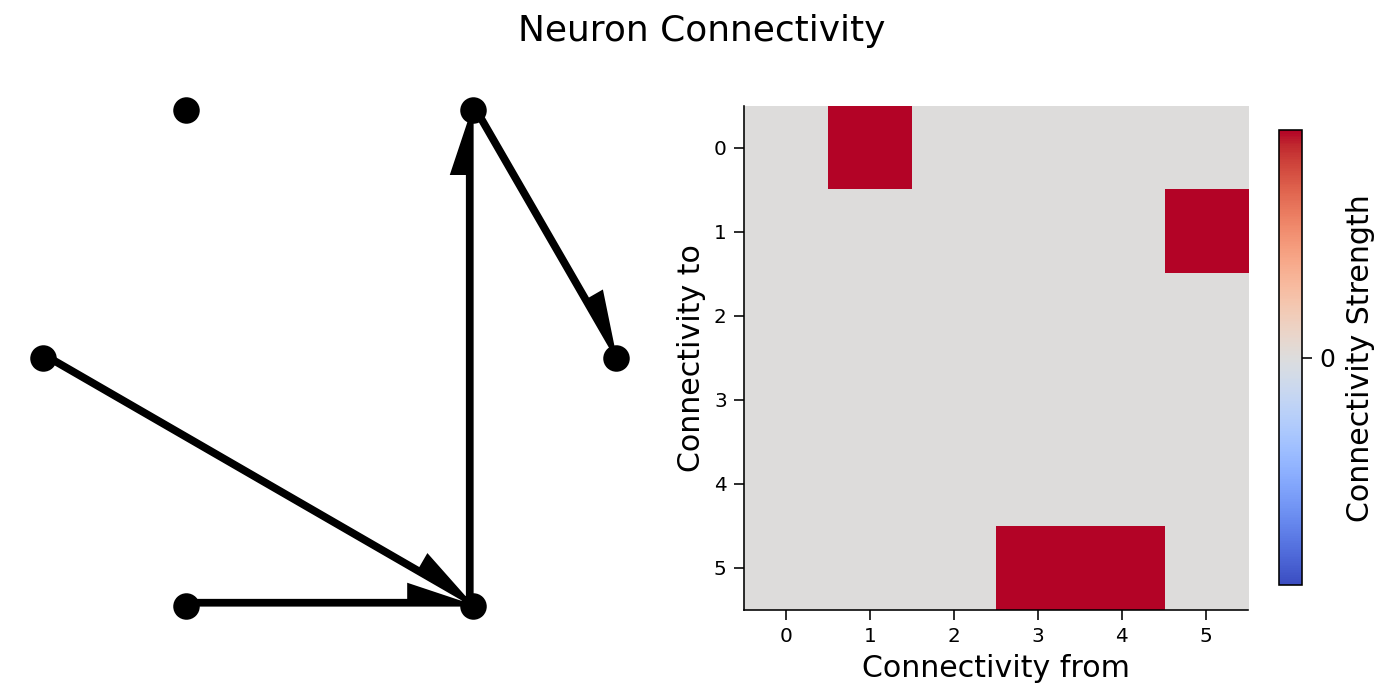
\includegraphics[scale=0.25]{Figures/NC/NC_Figure1.png}
\end{center}
\end{subbox}
\end{textbox}
%%%%%%%%%%%%%%%%%%%%%%%%% 
%%%%%%%%%%%%%%%%%%%%%%%%%
\begin{textbox}{\href{https://compneuro.neuromatch.io/tutorials/W3D5_NetworkCausality/student/W3D5_Tutorial1.html}{Interventions (W3D5T1)}   }
\begin{subbox}{subbox}{System simulation}
\scriptsize


To simulation a system of six neurons we using a sigmoid $\sigma$ function so that at every timestep the activity vector $x$ is updated according to: 
\begin{equation*}
\vec{x}_{t+1} = \sigma(A\vec{x}_t + \epsilon_t).
\end{equation*}
giving the plot:

\begin{center}
    
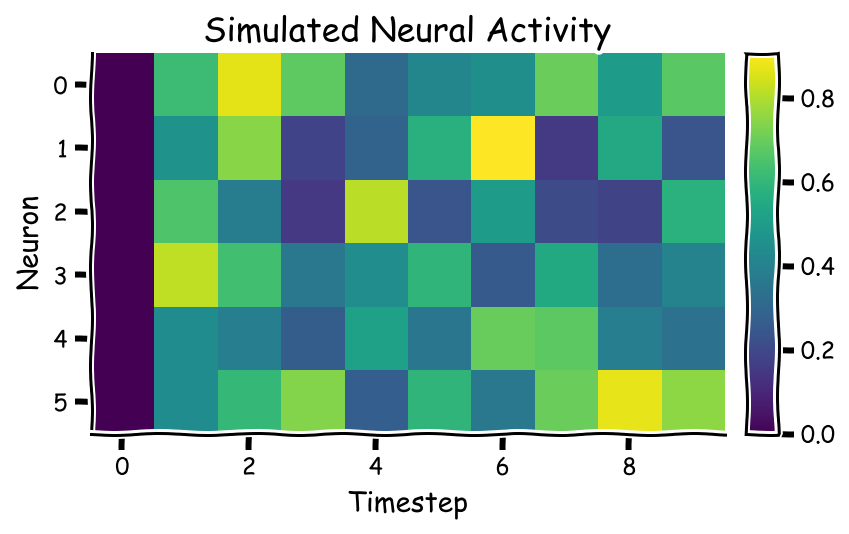
\includegraphics[scale=0.2]{Figures/NC/NC_Figure2.png}
\end{center}
\end{subbox}
\begin{subbox}{subbox}{Random perturbation in our system of neurons}
\scriptsize

We want to get the causal effect of each neuron upon each other neuron. The ground truth of the causal effects is the connectivity matrix $A$.

Remember that we would like to calculate:

\begin{eqnarray*}
\delta_{A\to B} &=& \mathbb{E}[B | A=1] -  \mathbb{E}[B | A=0] 
\end{eqnarray*}


We'll do this by randomly setting the system state to 0 or 1 and observing the outcome after one timestep. If we do this $N$ times, the effect of neuron $i$ upon neuron $j$ is:

\begin{eqnarray*}
\delta_{x^i\to x^j} &\approx& \frac1N \sum_{\substack{t=0, \ t \text{ even}}}^N[x_{t+1}^j | x^i_t=1] \\ & & - \frac1N \sum_{\substack{t=0, \ t \text{ even}}}^N[x_{t+1}^j | x^i_t=0]
\end{eqnarray*}

This is just the average difference of the activity of neuron $j$ in the two conditions.

We are going to calculate the above equation, but imagine it like \textit{intervening} in activity every other timestep.

\begin{center}
    
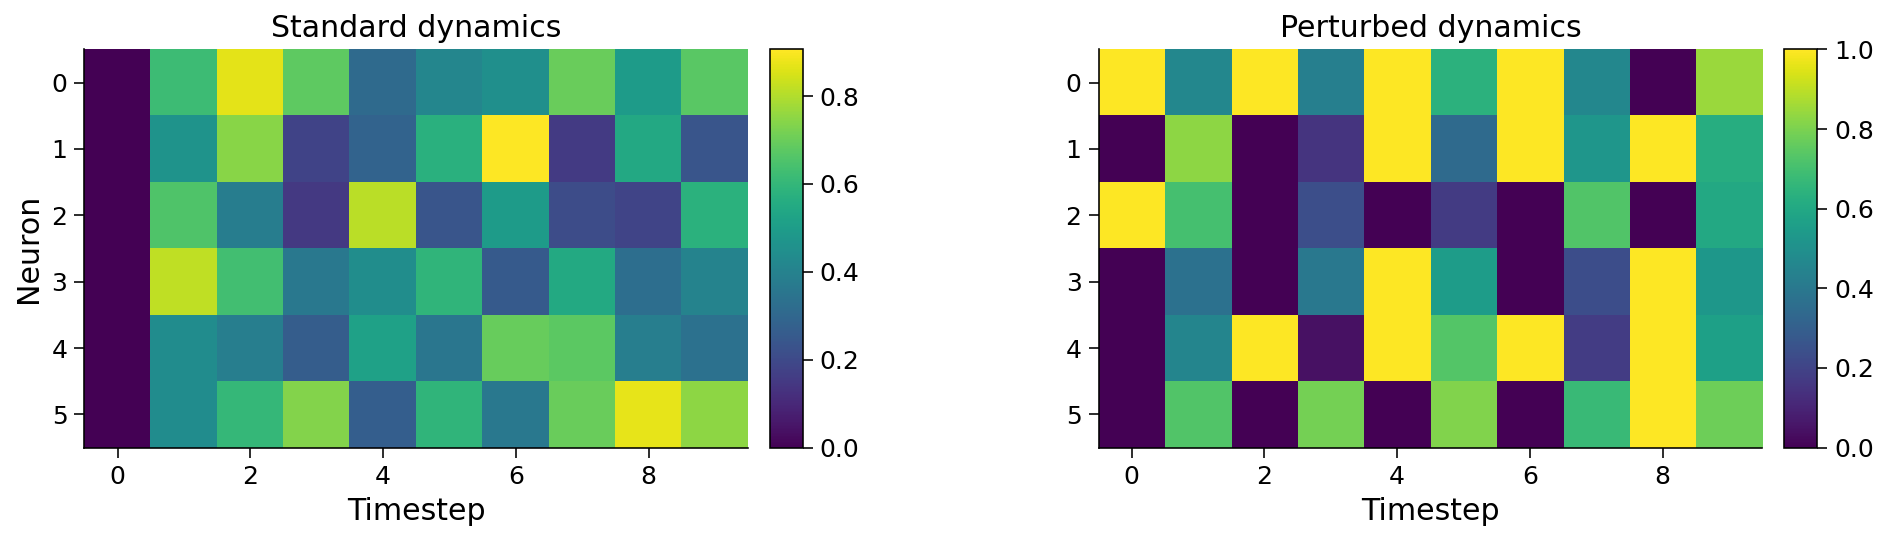
\includegraphics[scale=0.2]{Figures/NC/NC_Figure3.png}
\end{center}
\end{subbox}
\end{textbox}
%%%%%%%%%%%%%%%%%%%%%%%%% 
%%%%%%%%%%%%%%%%%%%%%%%%%
\begin{textbox}{\href{https://compneuro.neuromatch.io/tutorials/W3D5_NetworkCausality/student/W3D5_Tutorial1.html}{Interventions (W3D5T1)}   }

\begin{subbox}{subbox}{Recovering connectivity from perturbed dynamics}
\scriptsize

Recall that we perturbed every neuron at every other timestep. Despite perturbing every neuron, in this exercise we are concentrating on computing the causal effect of a single neuron (we will look at all neurons effects on all neurons next). We want to exclusively use the timesteps without perturbation for $x^j_{t+1}$ and the timesteps with perturbation for $x^j_{t}$ in the formulas above.

\begin{center}
    
\includegraphics[scale=0.15]{Figures/NC/NC_Figure4.png}
\end{center}
We can quantify how close our estimated connectivity matrix is to our true connectivity matrix by correlating them. We should see almost perfect correlation between our estimates and the true connectivity - do we?

\textbf{Note on interpreting A}: Strictly speaking, $A$ is not the matrix of causal effects but rather the dynamics matrix. So why compare them like this? The answer is that $A$ and the effect matrix both are $0$ everywhere except where there is a directed connection. So they should have a correlation of $1$ if we estimate the effects correctly. (Their scales, however, are different. This is in part because the nonlinearity $\sigma$ squashes the values of $x$ to $[0,1]$.) 
\begin{center}
    
\includegraphics[scale=0.2]{Figures/NC/NC_Figure6.png}
\end{center}
\begin{center}
    
\includegraphics[scale=0.2]{Figures/NC/NC_Figure7.png}
\end{center}
We can again calculate the correlation coefficient between the elements of the two matrices.
If it is almost 1 we have done a good job recovering the true causality of the system!

\end{subbox}
\end{textbox}
\newpage
%%%%%%%%%%%%%%%%%%%%%%%%% 
%%%%%%%%%%%%%%%%%%%%%%%%%
%%% TUTORIAL 2
%%%%%%%%%%%%%%%%%%%%%%%%% 
%%%%%%%%%%%%%%%%%%%%%%%%%
\begin{textbox}{\href{https://compneuro.neuromatch.io/tutorials/W3D5_NetworkCausality/student/W3D5_Tutorial2.html}{Correlations (W3D5T2)}   }

\begin{subbox}{subbox}{Recovering connectivity from perturbed dynamics}
\scriptsize


Here, we implemented and explored the dynamical system of neurons we will be working with throughout all of the tutorials today. We also learned about the "gold standard" of measuring causal effects through random perturbations. As random perturbations are often not possible, we will now turn to alternative methods to attempt to measure causality. We will:

\begin{itemize}
    \item  Learn how to estimate connectivity from observations assuming \textbf{correlations approximate causation}
\item Show that this only works when the network is small
\end{itemize}


Often, we can't force neural activities or brain areas to be on or off. We just have to observe. Maybe we can get the correlation between two nodes -- is that good enough? The question we ask here is \textbf{when is correlation a "good enough" substitute for causation?}

The answer is not "never", actually, but "sometimes".
\end{subbox}
\begin{subbox}{subbox}{Try to approximate causation with correlation}
\scriptsize



In small systems, correlation can look like causation. Let's attempt to recover the true connectivity matrix (A) just by correlating the neural state at each timestep with the previous state: $$C=\vec{x_t}{\vec{x_{t+1}}^\top}.$$ 

To calculate the connectivity matrix of a single neuron by calculating the correlation coefficients with every other neuron which correlate two vectors: 1) the activity of a selected neuron at time $t$ 2) The activity of all other neurons at time $t+1$.

The matrix answer is the same as the summation form.
Furthermore the estimated vs true connectivity look the same using the matrix calculation.

\begin{center}
    
\includegraphics[scale=0.2]{Figures/NC/NC_Figure9.png}
    
\includegraphics[scale=0.2]{Figures/NC/NC_Figure10.png}
\end{center}
\end{subbox}
\end{textbox}
%%%%%%%%%%%%%%%%%%%%%%%%%
%%%%%%%%%%%%%%%%%%%%%%%%%
\begin{textbox}{\href{https://compneuro.neuromatch.io/tutorials/W3D5_NetworkCausality/student/W3D5_Tutorial2.html}{Correlations (W3D5T2)}   }

\begin{subbox}{subbox}{Large systems}
\scriptsize

As our system becomes more complex however, correlation fails to capture causality.
Let's jump to a much bigger system. Instead of 6 neurons, we will now use 100 neurons. How does the estimation quality of the connectivity matrix change? 
\begin{center}

\includegraphics[scale=0.18]{Figures/NC/NC_Figure11.png}
\end{center}
\end{subbox}

\begin{subbox}{subbox}{Correlation as a function of network size}
\scriptsize
\begin{center}

\includegraphics[scale=0.15]{Figures/NC/NC_Figure13.png}
\end{center}
\end{subbox}
\begin{subbox}{subbox}{Connectivity estimation as a function of the sparsity of $A$}
\scriptsize

You may rightly wonder if correlation only fails for large systems for certain types of $A$. Does connectivity estimation get better or worse with less sparsity?

\begin{center}

\includegraphics[scale=0.15]{Figures/NC/NC_Figure12.png}
\end{center}
\end{subbox}

\begin{subbox}{subbox}{Summary}
\scriptsize


Now for the takeaway. We know that for large systems correlation $\not=$ causation. But what about when we coarsely sample the large system? Do we get better at estimating the effective causal interaction between groups (=average of weights) from the correlation between the groups?

From our simulation above, the answer appears to be no: as the number of neurons per group increases, we don't see any significant increase in our ability to estimate the causal interaction between groups.

\end{subbox}
\end{textbox}
\newpage
%%%%%%%%%%%%%%%%%%%%%%%%%
%%%%%%%%%%%%%%%%%%%%%%%%%
%%%% TUTORIAL 3
%%%%%%%%%%%%%%%%%%%%%%%%%
%%%%%%%%%%%%%%%%%%%%%%%%%
\begin{textbox}{\href{https://compneuro.neuromatch.io/tutorials/W3D5_NetworkCausality/student/W3D5_Tutorial3.html}{Simultaneous fitting/regression (W3D5T3)}   }

\begin{subbox}{subbox}{Objectives}
\scriptsize


We have explored correlation as an approximation for causation and learned that correlation $\neq$ causation for larger networks. However, computing correlations is a rather simple approach, and you may be wondering: will more sophisticated techniques allow us to better estimate causality? Can't we control things? 

Here we'll use some common advanced (but controversial) methods that estimate causality from observational data. These methods rely on fitting a function to our data directly, instead of trying to use perturbations or correlations. Since we have the full closed-form equation of our system, we can try these methods and see how well they work in estimating causal connectivity when there are no perturbations. Specifically, we will:

\begin{itemize}
    \item  Learn about more advanced (but also controversial) techniques for estimating causality
    \item conditional probabilities (\textbf{regression})
\item Explore limitations and failure modes
    \item  understand the problem of \textbf{omitted variable bias}
\end{itemize}

\end{subbox}

\begin{subbox}{subbox}{Regression approach}
\scriptsize

You may be familiar with the idea that correlation only implies causation when there are no hidden \textit{confounders}. This aligns with our intuition that correlation only implies causality when no alternative variables could explain away a correlation.

\textbf{A confounding example}:\\
Suppose you observe that people who sleep more do better in school. It's a nice correlation. But what else could explain it? Maybe people who sleep more are richer, don't work a second job, and have time to actually do homework. If you want to ask if sleep \textit{causes} better grades, and want to answer that with correlations, you have to control for all possible confounds.\\

A confound is any variable that affects both the outcome and your original covariate. In our example, confounds are things that affect both sleep and grades. 

\textbf{Controlling for a confound}: 
Confounds can be controlled for by adding them as covariates in a regression. But for your coefficients to be causal effects, you need three things:
 \begin{enumerate}
     \item 
 All confounds are included as covariates
\item  Your regression assumes the same mathematical form of how covariates relate to outcomes (linear, GLM, etc.)
\item  No covariates are caused *by* both the treatment (original variable) and the outcome. These are \href{https://en.wikipedia.org/wiki/Collider_(statistics)}{colliders}; we won't introduce it today (but Google it on your own time! Colliders are very counterintuitive.)
 \end{enumerate}

In the real world it is very hard to guarantee these conditions are met. In the brain it's even harder (as we can't measure all neurons). Luckily today we simulated the system ourselves.

\end{subbox}
\end{textbox}
%%%%%%%%%%%%%%%%%%%%%%%%%
%%%%%%%%%%%%%%%%%%%%%%%%%
\begin{textbox}{\href{https://compneuro.neuromatch.io/tutorials/W3D5_NetworkCausality/student/W3D5_Tutorial3.html}{Simultaneous fitting/regression (W3D5T3)}   }

\begin{subbox}{subbox}{Fitting a General Linear Model (GLM)}
\scriptsize
We will use a regression approach to estimate the causal influence of all neurons to neuron #1. Specifically, we will use linear regression to determine the $A$ in:
\begin{equation}
\sigma^{-1}(\vec{x}_{t+1}) = A\vec{x}_t + \epsilon_t ,
\end{equation}
where $\sigma^{-1}$ is the inverse sigmoid transformation, also sometimes referred to as the \textbf{logit} transformation: $\sigma^{-1}(x) = \log(\frac{x}{1-x})$.

Let $W$ be the $\vec{x}_t$ values, up to the second-to-last timestep $T-1$:
\begin{equation}
W = 
\begin{bmatrix}
\mid & \mid & ... & \mid \\ 
\vec{x}_0  & \vec{x}_1  & ... & \vec{x}_{T-1}  \\ 
\mid & \mid & ... & \mid
\end{bmatrix}_{n \times (T-1)}
\end{equation}

Let $Y$ be the $\vec{x}_{t+1}$ values for a selected neuron, indexed by $i$, starting from the second timestep up to the last timestep $T$:

\begin{equation}
Y = 
\begin{bmatrix}
x_{i,1}  & x_{i,2}  & ... & x_{i, T}  \\ 
\end{bmatrix}_{1 \times (T-1)}
\end{equation}

You then fit the following model:

\begin{equation}
\sigma^{-1}(Y^T) = W^TV
\end{equation}

where $V$ is the $n \times 1$ coefficient matrix of this regression, which will be the estimated connectivity matrix between the selected neuron and the rest of the neurons.


We can see that multiple regression is better than simple correlation for estimating connectivity.


\end{subbox}

\end{textbox}
%%%%%%%%%%%%%%%%%%%%%%%%%
%%%%%%%%%%%%%%%%%%%%%%%%%
\begin{textbox}{\href{https://compneuro.neuromatch.io/tutorials/W3D5_NetworkCausality/student/W3D5_Tutorial3.html}{Simultaneous fitting/regression (W3D5T3)}   }

\begin{subbox}{subbox}{Partially Observed Systems}
\scriptsize
If we are unable to observe the entire system, \textbf{omitted variable bias} becomes a problem. If we don't have access to all the neurons, and so therefore can't control them, can we still estimate the causal effect accurately?

We first visualize different subsets of the connectivity matrix when we observe 75\% of the neurons vs 25\%.

Recall the meaning of entries in our connectivity matrix: $A[i,j] = 1$ means a connectivity from neuron $i$ to neuron $j$ with strength $1$.
\begin{center}
    
\includegraphics[scale=0.24]{Figures/NC/NC_Figure15.png}

\end{center}

Next, we will inspect a plot of the correlation between true and estimated connectivity matrices vs the percent of neurons observed over multiple trials.
What is the relationship that you see between performance and the number of neurons observed?

\begin{center}
    
\includegraphics[scale=0.25]{Figures/NC/NC_Figure17.png}

\end{center}
\end{subbox}

\end{textbox}
\newpage
%%%%%%%%%%%%%%%%%%%%%%%%%
%%%%%%%%%%%%%%%%%%%%%%%%%
%%%% TUTORIAL 4
%%%%%%%%%%%%%%%%%%%%%%%%%
%%%%%%%%%%%%%%%%%%%%%%%%%
\begin{textbox}{\href{https://compneuro.neuromatch.io/tutorials/W3D5_NetworkCausality/student/W3D5_Tutorial4.html}{Instrumental Variables (W3D5T4)}   }

\begin{subbox}{subbox}{Objectives}
\scriptsize


We have seen that even more sophisticated techniques such as simultaneous fitting fail to capture causality in the presence of omitted variable bias. So what techniques are there for us to obtain valid causal measurements when we can't perturb the system? Here we will:
\begin{itemize}
    \item 
 learn about \textbf{instrumental variables}, a method that does not require experimental data for valid causal analysis
\item  explore benefits of instrumental variable analysis and limitations
 \item  addresses \textbf{omitted variable bias} seen in regression
   \item  less efficient in terms of sample size than other techniques
 \item  requires a particular form of randomness in the system in order for causal effects to be identified
    \end{itemize}

\end{subbox}

\begin{subbox}{subbox}{Instrumental Variables}
\scriptsize

If there is randomness naturally occurring in the system \textit{that we can observe}, this in effect becomes the perturbations we can use to recover causal effects. This is called an \textbf{instrumental variable}. At high level, an instrumental variable must
\begin{enumerate}
    
\item Be observable
\item  Affect a covariate you care about
\item  \textbf{Not} affect the outcome, except through the covariate
\end{enumerate}

It's rare to find these things in the wild, but when you do it's very powerful.
\begin{center}
    
\includegraphics[scale=0.15]{Figures/NC/NC_Figure18.png}

\end{center}
\end{subbox}
\end{textbox}
%%%%%%%%%%%%%%%%%%%%%%%%%%%%%%%%%%
%%%%%%%%%%%%%%%%%%%%%%%%%
\begin{textbox}{\href{https://compneuro.neuromatch.io/tutorials/W3D5_NetworkCausality/student/W3D5_Tutorial4.html}{Instrumental Variables (W3D5T4)}   }
\begin{subbox}{subbox}{A non-neuro example of an Instrumental Variables (IV)}
\scriptsize

A classic example is estimating the effect of smoking cigarettes while pregnant on the birth weight of the infant. There is a (negative) correlation, but is it causal? Unfortunately many confounds affect both birth weight and smoking. Wealth is a big one. Instead of controlling everything imaginable, one can find an IV. Here the instrumental variable is \textbf{state taxes on tobacco}. These

\begin{enumerate}
    \item    Are observable
    \item   Affect tobacco consumption
    \item   Don't affect birth weight except through tobacco
\end{enumerate}

By using the power of IV techniques, you can determine the causal effect without exhaustively controlling for everything.

Let's represent our tobacco example above with the following notation:
\begin{itemize}
    \item 
 $Z_{\text{taxes}}$: our tobacco tax \textit{instrument}, which only affects an individual's tendency to smoke while pregnant within our system
\item $T_{\text{smoking}}$: number of cigarettes smoked per day while pregnant, our "treatment" if this were a randomized trial
\item $C_{\text{SES}}$: socioeconomic status (higher means wealthier), a \textit{confounder} if it is not observed
\item
$Y_{\text{birthweight}}$: child birthweight in grams, our outcome of interest
\end{itemize}

Let's suppose we have the following function for our system:
$$Y_{\text{birthweight}} = 3000 + C_{\text{SES}} - 2T_{\text{smoking}},$$
with the additional fact that $C_{\text{SES}}$ is negatively correlated with $T_{\text{smoking}}$. 

The causal effect we wish to estimate is the coefficient $-2$ for $T_{\text{smoking}}$, which means that if a mother smokes one additional cigarette per day while pregnant her baby will be 2 grams lighter at birth. We've provided a covariance matrix with the desired structure in the code cell below, so please run it to look at the correlations between our variables.\\
Correlation between SES status and cigarettes: -0.483\\
Correlation between SES status and birth weight: 0.740\\
We see what is exactly represented in our graph above: $C_{\text{SES}}$ is correlated with both $T_{\text{smoking}}$ and $Y_{\text{birthweight}}$, so $C_{\text{SES}}$ is a potential confounder if not included in our analysis. Let's say that it is difficult to observe and quantify $C_{\text{SES}}$, so we do not have it available to regress against. This is another example of the \textbf{omitted variable bias}.\\
What about $Z_{\text{taxes}}$?\\
Correlation between taxes and cigarettes: 0.519\\
Correlation between taxes and SES status: 0.009\\
Perfect! We see that $Z_{\text{taxes}}$ is correlated with $T_{\text{smoking}}$ (#2) but is uncorrelated with $C_{\text{SES}}$ (#3).  $Z_\text{taxes}$ is also observable (#1), so we've satisfied our three criteria for an instrument:
\begin{enumerate}
    \item 
   $Z_\text{taxes}$ is observable
\item    $Z_\text{taxes}$ affects $T_{\text{smoking}}$
\item    $Z_\text{taxes}$ doesn't affect
\end{enumerate}
$Y_{\text{birthweight}}$ except through $T_{\text{smoking}}$ (ie $Z_\text{taxes}$ doesn't affect or is affected by $C_\text{SES}$)

\end{subbox}
\end{textbox}
%%%%%%%%%%%%%%%%%%%%%%%%%
%%%%%%%%%%%%%%%%%%%%%%%%%
\begin{textbox}{\href{https://compneuro.neuromatch.io/tutorials/W3D5_NetworkCausality/student/W3D5_Tutorial4.html}{Instrumental Variables (W3D5T4)}   }
\begin{subbox}{subbox}{ How IV works, at high level
}
\scriptsize
The easiest way to imagine IV is that the instrument is \textbf{an observable source of "randomness"} that affects the treatment. In this way it's similar to the interventions we talked about in Tutorial 1.

But how do you actually use the instrument? The key is that we need to extract \textbf{the component of the treatment that is due only to the effect of the instrument}. We will call this component $\hat{T}$.
$$
\hat{T}\leftarrow \text{The unconfounded component of }T
$$
Getting $\hat{T}$ is fairly simple. It is simply the predicted value of $T$ found in a regression that has only the instrument $Z$ as input.

Once we have the unconfounded component in hand, getting the causal effect is as easy as regressing the outcome on $\hat{T}$.

\end{subbox}
\begin{subbox}{subbox}{ IV estimation using two-stage least squares
}
\scriptsize
The fundamental technique for instrumental variable estimation is \textbf{two-stage least squares}. 

We run two regressions:
\begin{enumerate}
    \item 
 The first stage gets  $\hat{T}_{\text{smoking}}$ by regressing $T_{\text{smoking}}$ on $Z_\text{taxes}$, fitting the parameter $\hat{\alpha}$:

\begin{equation}
\hat{T}_{\text{smoking}} = \hat{\alpha} Z_\text{taxes}
\end{equation}

\item The second stage then regresses $Y_{\text{birthweight}}$ on $\hat{T}_{\text{smoking}}$ to obtain an estimate $\hat{\beta}$ of the causal effect:
\end{enumerate}

\begin{equation}
\hat{Y}_{\text{birthweight}} = \hat{\beta} \hat{T}_{\text{smoking}} 
\end{equation}

The first stage estimates the \textbf{unconfounded component} of $T_{\text{smoking}}$ (ie, unaffected by the confounder $C_{\text{SES}}$), as we discussed above. 

Then, the second stage uses this unconfounded component $\hat{T}_{\text{smoking}}$ to estimate the effect of smoking on $\hat{Y}_{\text{birthweight}}$. 

\textbf{Compute regression stage 1}\\

Let's run the regression of $T_{\text{smoking}}$ on $Z_\text{taxes}$ to compute $\hat{T}_{\text{smoking}}$. We will then check whether our estimate is still confounded with $C_{\text{SES}}$ by comparing the correlation of $C_{\text{SES}}$  with $T_{\text{smoking}}$ vs $\hat{T}_{\text{smoking}}$.\\
The result of the correlation between $T$ and $C$ of `-0.483` and between $\hat{T}$ and $C$ of `0.009`.\\

\textbf{Least squares regression stage 2}\\
Now let's implement the second stage! We will again use a linear regression model with an intercept. We will obtain the estimated causal effect of the number of cigarettes ($T$) on birth weight ($Y$).\\

The result of estimated causal effect of `-1.984`, This is quite close to the true causal effect of $-2$!

\end{subbox}
\end{textbox}
%%%%%%%%%%%%%%%%%%%%%%%%%
%%%%%%%%%%%%%%%%%%%%%%%%%
\begin{textbox}{\href{https://compneuro.neuromatch.io/tutorials/W3D5_NetworkCausality/student/W3D5_Tutorial4.html}{Instrumental Variables (W3D5T4)}   }
\begin{subbox}{subbox}{ IVs in our simulated neural system
}
\scriptsize
Now, say we have the neural system we have been simulating, except with an additional variable $\vec{z}$. This will be our instrumental variable. 

We treat $\vec{z}$ as a source of noise in the dynamics of our neurons:

\begin{equation}
\vec{x}_{t+1} = \sigma(A\vec{x}_t + \eta \vec{z}_{t+1} + \epsilon_t)
\end{equation}

where $\eta$ is what we'll call the "strength" of our IV, and $\vec{z}_t$ is a random binary variable, $\vec{z}_t \sim Bernoulli(0.5)$

Remember that for each neuron $i$, we are trying to figure out whether $i$ is connected to (causally affects) the other neurons in our system *at the next time step*. So for timestep $t$, we want to determine whether $\vec{x}_{i,t}$ affects all the other neurons at $\vec{x}_{t+1}$. For a given neuron $i$, $\vec{z}_{i,t}$ satisfies the 3 criteria for a valid instrument. \\

\textbf{What could $z$ be, biologically?}\\

Imagine $z$ to be some injected current through an \textit{in vivo} patch clamp. It affects each neuron individually, and only affects dynamics through that neuron.

The cool thing about IV is that you don't have to control $z$ yourself - it can be observed. So if you mess up your wiring and accidentally connect the injected voltage to an AM radio, no worries. As long as you can observe the signal the method will work.
\begin{center}
    
\includegraphics[scale=0.1]{Figures/NC/NC_Figure19.png}

\end{center}
\end{subbox}
\begin{subbox}{subbox}{  Simulate a system with IV
}
\scriptsize

\begin{center}
    
\includegraphics[scale=0.2]{Figures/NC/NC_Figure20.png}

\end{center}
\end{subbox}

\end{textbox}
%%%%%%%%%%%%%%%%%%%%%%%%%
%%%%%%%%%%%%%%%%%%%%%%%%%
\begin{textbox}{\href{https://compneuro.neuromatch.io/tutorials/W3D5_NetworkCausality/student/W3D5_Tutorial4.html}{Instrumental Variables (W3D5T4)}   }
\begin{subbox}{subbox}{ Estimate IV for simulated neural system
}
\scriptsize
Since you just implemented two-stage least squares, let's see how our IV estimates do in recovering the connectivity matrix.
\begin{center}
    
\includegraphics[scale=0.2]{Figures/NC/NC_Figure21.png}

\end{center}
The IV estimates seem to perform pretty well! In the next section, we will see how they behave in the face of omitted variable bias.

\end{subbox}

\begin{subbox}{subbox}{ IVs and omitted variable bias
}
\scriptsize
Changing the ratio of observed neurons and look at the impact on the quality of connectivity estimation using IV vs regression. The plots below are for a ratio of 0.6.

\begin{center}
    
\includegraphics[scale=0.16]{Figures/NC/NC_Figure22.png}

\end{center}
We can also visualize the performance of regression and IV as a function of the observed neuron ratio below.

\begin{center}
\includegraphics[scale=0.2]{Figures/NC/NC_Figure23.png}

\end{center}

We see that IVs handle omitted variable bias (when the instrument is strong and we have enough data).

\textbf{The costs of IV analysis}
\begin{itemize}
    

\item  we need to find an appropriate and valid instrument
\item  Because of the 2-stage estimation process, we need strong instruments or else our standard errors will be large
\end{itemize}
\end{subbox}
\end{textbox}
%%%%%%%%%%%%%%%%%%%%%%%%%
%%%%%%%%%%%%%%%%%%%%%%%%%
\end{multicols}
\end{document}
